%% LLT: Turn off some annoying warnings...
\RequirePackage{silence}
\WarningFilter{titlesec}{Non standard sectioning command}
\WarningFilter{scrreprt}{Usage of package}
\WarningFilter{scrreprt}{Activating an ugly workaround}

% **************************************************
% Document Class Definition
% **************************************************
\documentclass[%
	paper=A4,					% paper size --> A4 is default in Germany
	twoside=true,				% onesite or twoside printing
	openright,					% doublepage cleaning ends up right side
	parskip=full,				% spacing value / method for paragraphs
	chapterprefix=true,			% prefix for chapter marks
	11pt,						% font size
	headings=normal,			% size of headings
	bibliography=totoc,			% include bib in toc
	listof=totoc,				% include listof entries in toc
	titlepage=on,				% own page for each title page
	captions=tableabove,		% display table captions above the float env
	draft=false,				% value for draft version
]{scrreprt}%

% **************************************************
% Debug LaTeX Information
% **************************************************
%\listfiles

% **************************************************
% Information and Commands for Reuse
% **************************************************
\newcommand{\thesisTitle}{Interactive Visualization within the Reality-Virtuality Continuum to Support Motor Skill Learning and Education}
\newcommand{\thesisName}{Florian Diller}
\newcommand{\thesisSubject}{Documentation}
\newcommand{\thesisDate}{May 12, 2025}
\newcommand{\thesisVersion}{1.2}

\newcommand{\thesisFirstReviewer}{Prof. Dr. Alexander Wiebel}
\newcommand{\thesisFirstReviewerUniversity}{\protect{Worms University of Applied Sciences}}
\newcommand{\thesisFirstReviewerDepartment}{Department of Computer Science}

\newcommand{\thesisSecondReviewer}{Prof. Dr. Gerik Scheuermann}
\newcommand{\thesisSecondReviewerUniversity}{\protect{Leipzig University}}
\newcommand{\thesisSecondReviewerDepartment}{Department of Computer Science}

\newcommand{\thesisFirstSupervisor}{Prof. Dr. Alexander Wiebel}
\newcommand{\thesisSecondSupervisor}{Prof. Dr. Gerik Scheuermann}

\newcommand{\thesisUniversity}{\protect{Leipzig\\University}}
\newcommand{\thesisUniversityDepartment}{Department of Computer Science}
\newcommand{\thesisUniversityInstitute}{BSV Research Group}
\newcommand{\thesisUniversityGroup}{BSV Research Group}
\newcommand{\thesisUniversityCity}{Leipzig}
\newcommand{\thesisUniversityStreetAddress}{Augustplatz 10}
\newcommand{\thesisUniversityPostalCode}{04109}

\newcommand{\supervisionUniversity}{\protect{Worms\\University of Applied Sciences}}
\newcommand{\supervisionUniversityDepartment}{Department of Computer Science}
\newcommand{\supervisionUniversityInstitute}{UX-Vis Research Group}
\newcommand{\supervisionUniversityGroup}{UX-Vis Research Group}

% **************************************************
% Load and Configure Packages
% **************************************************
\usepackage[utf8]{inputenc}		% defines file's character encoding
\usepackage[english]{babel} % babel system, adjust the language of the content
\usepackage[					% clean thesis style
	figuresep=colon,%
	sansserif=false,%
	hangfigurecaption=false,%
	hangsection=true,%
	hangsubsection=true,%
	colorize=full,%
	colortheme=bluemagenta,%
% LLT: Use biber if using UTF8 encoding
 	bibsys=bibtex,%
	%bibsys=biber,%
	configurebiblatex=true,
	bibfile=bib-refs,%
	bibstyle=numeric,%
]{cleanthesis}
\usepackage{biblatex}

%--------------------Florian's packages--------------------%
\usepackage{subfig}
\usepackage{rotating}
\usepackage{hyperref}
\usepackage{multirow} %used for table
\usepackage{tabu}  %used for table
\usepackage{booktabs} %used for table

\usepackage{soul}

%%%% OUR Commands
\newcommand{\todo}[1]{\textcolor{white}{\colorbox{red}{ Noch zu %
      tun:}}\ \ \textcolor{orange}{#1} \textcolor{red}{\colorbox{red}{I}}\ \ }

\newcommand{\eg}{e.\,g.}
\newcommand{\ie}{i.\,e.}
\newcommand{\etal}{et~al.}
\newcommand{\basedOn}[1]{{\textcolor{lightgray}{{\bfseries Der obige Text basiert auf folgenden Notizen:}\ \ #1 \ }}}
\newcommand{\toWrite}[1]{{\textcolor{gray}{{\bfseries To write:}\ \ #1 \ }}}

\usepackage[normalem]{ulem}
\newcommand{\fd}[1]{\textcolor{cyan}{#1}}
\newcommand{\fds}[1]{\marginpar{\tiny\textcolor{cyan}{{\bfseries Flo says}: ''#1''}}}
\newcommand{\fdn}[2]{{\sethlcolor{cyan}\hl{#1}}\marginpar{\tiny\textcolor{blue}{\vskip-10mm{\bfseries Flo notes}: ''#2''}}}

\newcommand{\ros}[1]{\marginpar{\tiny\textcolor{red}{{\bfseries Reviewer1}: ''#1''}}}
\newcommand{\rts}[1]{\marginpar{\tiny\textcolor{red}{{\bfseries Reviewer2}: ''#1''}}}
\newcommand{\rths}[1]{\marginpar{\tiny\textcolor{red}{{\bfseries Reviewer3}: ''#1''}}}
\newcommand{\rss}[1]{\marginpar{\tiny\textcolor{green}{{\bfseries Reviewer3}: ''#1''}}}

\newcommand{\aw}[1]{\textcolor{orange}{#1}}
\newcommand{\awr}[2]{\textcolor{gray}{{\bf Reviewer#1:} #2}}
\newcommand{\aws}[1]{\marginpar{\tiny\textcolor{orange}{{\bfseries Alex says}: ''#1''}}}
\newcommand{\awn}[2]{{\sethlcolor{orange}\hl{#1}}\marginpar{\tiny\textcolor{orange}{\vskip-10mm{\bfseries Alex notes}: ''#2''}}}
\newcommand{\awnb}[2]{{\textcolor{white}{\sethlcolor{blue}\hl{#1}}}\marginpar{\tiny\textcolor{blue}{{\bfseries Alex notes}: ''#2''}}}
\newcommand{\awnr}[2]{{\hl{#1}}\marginpar{\tiny\textcolor{red}{{\bfseries Alex notes}: ''#2''}}}

\newcommand{\on}[2]{{\color{red}{\st{#1}}}{{\color{blue}{\ul{#2}}}}}%on=old/new
%\newcommand{\on}[2]{{#1}}%on=old/new

\newcommand{\formulation}[1]{\uwave{#1}}

\usepackage{tikz}
\def\checkmark{\tikz\fill[scale=0.4](0,.35) -- (.25,0) -- (1,.7) -- (.25,.15) -- cycle;}

\usepackage{xr}
\usepackage{comment}
\usepackage{graphicx}
\usepackage[acronym, nonumberlist=false, nogroupskip]{glossaries}
\usepackage{multicol}


\renewcommand{\cfttoctitlefont}{\thesischapterfont}
\renewcommand{\cftchapfont}{\normalfont\bfseries}
\renewcommand{\cftloftitlefont}{\thesischapterfont}
\renewcommand{\cftlottitlefont}{\thesischapterfont}

\newcommand{\Autoref}[1]{\begingroup
  \def\sectionautorefname{Section}%
  \autoref{#1}%
\endgroup}

\makeglossaries

\hypersetup{					% setup the hyperref-package options
	pdftitle={\thesisTitle},	% 	- title (PDF meta)
	pdfsubject={\thesisSubject},% 	- subject (PDF meta)
	pdfauthor={\thesisName},	% 	- author (PDF meta)
	plainpages=false,			% 	-
	colorlinks=false,			% 	- colorize links?
	pdfborder={0 0 0},			% 	-
	breaklinks=true,			% 	- allow line break inside links
	bookmarksnumbered=true,		%
	bookmarksopen=true			%
}

% **************************************************
% Document CONTENT
% **************************************************
\begin{document}
% --------------------------
% rename document parts
% --------------------------
%\renewcaptionname{ngerman}{\figurename}{Abb.}
%\renewcaptionname{ngerman}{\tablename}{Tab.}
\renewcaptionname{english}{\figurename}{Fig.}
\renewcaptionname{english}{\tablename}{Tab.}

\newacronym{vr}{VR}{Virtual Reality}
\newacronym{ar}{AR}{Augmented Reality}
\newacronym{xr}{XR}{Extended Reality}
\newacronym{mr}{MR}{Mixed Reality}
\newacronym[plural=HMDs, firstplural=Head-Mounted Displays]{hmd}{HMD}{Head-Mounted Display}
\newacronym{rmd}{RMD}{Room-Mounted Display}
\newacronym{pca}{PCA}{Principal Component Analysis}
\newacronym{cg}{CG}{Computer Graphics}
\newacronym{gan}{GAN}{Generative Adversarial Networks}
\newacronym{ml}{ML}{Machine Learning}
\newacronym{oer}{OER}{Open Educational Resources}
\newacronym{pov}{POV}{Point of View}
\newacronym{cave}{CAVE}{Cave Automatic Virtual Environment}
\newacronym{vse}{VSE}{Viewpoint Selection Error}
\newacronym{jmo}{JMO}{Joint Mutual Occlusion}
\newacronym{usd}{USD}{United States Dollar}
\newacronym{m}{M}{Mean}
\newacronym{mdn}{Mdn}{Median}
\newacronym{sd}{SD}{Standard Deviation}
\newacronym{un}{UN}{United Nations}
\newacronym{unesco}{UNESCO}{United Nations Educational, Scientific and Cultural Organization}
\newacronym{ui}{UI}{User Interface}
\newacronym{ux}{UX}{User Experience}
\newacronym{plato}{PLATO}{Programmed Logic for Automatic Teaching Operations}
\newacronym{cgems}{CGEMS}{Computer Graphics Educational Materials Source}
\newacronym{acm}{ACM}{Association for Computing Machinery}
\newacronym{siggraph}{SIGGRAPH}{Special Interest Group on Graphics and Interactive Techniques}
\newacronym{dda}{DDA}{Digital Differential Analyzer}
\newacronym{prisma}{PRISMA}{Preferred Reporting Items for Systematic Reviews and Meta-Analyses}
\newacronym{ieee}{IEEE}{Institute of Electrical and Electronics Engineers}
\newacronym{hci}{HCI}{Human Computer Interaction}
\newacronym{6dof}{6DoF}{Six Degrees of Freedom}
\newacronym{usb}{USB}{Universal Serial Bus}

% --------------------------
% Front matter
% --------------------------
\pagenumbering{roman}			% roman page numbing (invisible for empty page style)
\pagestyle{empty}				% no header or footers
% !TEX root = ../thesis-example.tex
%
% ------------------------------------  --> cover title page
\begin{titlepage}
	\pdfbookmark[0]{Cover}{Cover}
	\flushright
	\hfill
	\vfill
	{\LARGE\thesisTitle \par}
	\rule[5pt]{\textwidth}{.4pt} \par
	{\Large\thesisName}
	\vfill
	\textit{\large\thesisDate} \\
	Version: \thesisVersion
\end{titlepage}


% ------------------------------------  --> main title page

\begin{titlepage}
	\pdfbookmark[0]{Titlepage}{Titlepage}
	\normalfont
	%\tgherosfont
	\centering

	\vfill
	\vspace*{15mm}
	{\tgherosfont \huge \thesisTitle \\[10mm]}
	%\normalfont
	{\large Der Fakultät für Mathematik und Informatik}\\
	{\large der Universität Leipzig}\\
	{\large eingereichte}\\[10mm]
	{\large DISSERTATION}\\[10mm]
	{\large zur Erlangung des akademischen Grades}\\[7mm]
	{\large DOCTOR RERUM NATURALIUM}\\
	{\large (Dr. rer. nat.)}\\[7mm]
	{\large im Fachgebiet}\\[7mm]
	{\large INFORMATIK}\\[7mm]
	{\large vorgelegt}\\[10mm]
	{\large von M.Sc. Florian Diller}\\
	{\large geboren am 28.02.1990 in Mannheim}\\[20mm]
	\raggedright
	{\large \thesisUniversityCity, den \thesisDate}


\end{titlepage}


% ------------------------------------  --> lower title back for single page layout
\hfill
\vfill
{
	\small
	\textbf{\thesisName} \\
	\textit{\thesisTitle} \\
	\thesisSubject, \thesisDate \\
	%Reviewers: \thesisFirstReviewer\ and \thesisSecondReviewer \\
	Supervisors: \thesisFirstSupervisor\ and \thesisSecondSupervisor \\[1.5em]
	\textbf{\thesisUniversity} \\
	\textit{\thesisUniversityGroup} \\
	%\thesisUniversityInstitute \\
	\thesisUniversityDepartment \\
	\thesisUniversityStreetAddress \\
	\thesisUniversityPostalCode\ \thesisUniversityCity
}
		% INCLUDE: all titlepages
\cleardoublepage

\pagestyle{plain}				% display just page numbers
% !TEX root = ../thesis-example.tex
%
\externaldocument{content/survey}
\externaldocument{content/registration}
\externaldocument{content/viewpoint}
\externaldocument{content/ExGOER}
\externaldocument{content/omnipresent}
\pdfbookmark[0]{Abstract}{Abstract}
\chapter*{Abstract}
\label{sec:abstract}
\vspace*{-10mm}

The spectrum between real and virtual --- as represented by the reality-virtuality continuum according to Milgram --- offers an endless range of compelling opportunities for user interaction.
The work at hand explores novel visualization methods within the reality-virtuality continuum and how they can be leveraged to teach complex concepts in education and motor skill learning.
Moreover, interaction is of great importance for virtual learning.
Especially so-called experiential learning approaches can utilize interaction to form unique educational experiences for facilitating learning.
To motivate the topic and its underlying concepts, this thesis starts by exploring the educational background.
The concepts \emph{Experiential Learning}, \emph{Skill Learning} and \emph{Situated Learning} are introduced and linked to establish a connection to the overarching goal of teaching through virtual visual support in Mixed Reality.

Drawing on this foundation, a novel framework for education in an academic setting is presented.
The framework teaches complex theoretical concepts from the field of computer graphics through a holistic framework of interactive web applications, slides and quizzes.
A split test experiment with 19 students was conducted.
Among eight topics, two groups were formed: One conventionally repeating the topic with slides, the other with the interactive web application.
Testing the quiz score before and after repeating, suggested that the user group supported by the interactive web application improved more.
Additionally, the framework was shown to an UX-expert and teaching personnel, receiving positive responses throughout.
In this approach, the scope is held broad, emphasizing visual interactivity, usability and open access.

Subsequently, the scope is narrowed to provide deeper insight into a topic with complex temporal and spatial concepts to convey: \emph{Motor Skill Learning}.
This is achieved by initially providing a comprehensive literature overview of feedback based on visual cues in the field of motor skill learning in Mixed Reality.
The existing literature was analyzed from 2016 to the present, searching for AR and VR methods providing visual cues for corrective feedback in Mixed Reality.
This process resulted in 39 relevant papers, providing a diverse range of methods.
Moreover, the selected publications were classified according to their visual cues, Mixed Reality technologies and more.
As a result, it is possible to gain insight into the relationships between different aspects of feedback and the ways in which visual feedback is applied in Mixed Reality within the literature.
Additionally, the literature survey highlighted gaps in the research and therefore understanding of visual cues for motor skill learning in general.

Addressing these gaps, we identified one of the more prevalent visual cues in the surveyed literature for motor skill learning - superimposed human avatars.
In this context, when superimposing two human avatars for motor feedback, it is crucial how they are registered, as this represents the foundation of the differences in the poses or movements.
Therefore, a framework was developed to register superimposed human avatars and several exemplary exercises were provided.
Making sure a connection to the environment was established facilitated a better understanding of the target exercise in most cases.

Building upon this foundational knowledge, a method for viewpoint selection was developed.
This method considers feedback in real time by highlighting the visual cues depending on the discrepancy of actual and target movement.
Not only, does the method provide a thought-out compromise between a pose-optimized and a feedback-optimized viewpoint, it also ensures a smooth camera movement.
To compare the method to methods from the literature, a user study involving 39 individuals was conducted.
Users could select one of four videos, each optimized by a different method, including the one presented.
As a result, the presented method was most frequently selected as being the most informative.
Additionally, the method was computationally faster than previous viewpoint selection methods for human avatars.
Among the methods tested, it was the only one capable of running in real time.

Lastly, the work at hand presents a novel Augmented Reality feedback system for motor learning, which leverages an AR headset to provide visual motor feedback independent of head position.
As a result, this allows the user to receive motor feedback in a comfortable manner without risking an incorrect exercise execution.
The spatial positioning of the virtual feedback in AR is carefully designed to not irritate the user, cover various use cases, and provide a comfortable experience.
In addition, the system was evaluated in an in-subject user study with 32 participants, testing the system against conventional methods found in the literature.
For this purpose, the users solved two tasked: One where feedback had to be interpreted, and one where a pose had to be mimicked according to visual feedback.
Subsequently, a few structured questions were asked about the experience.
There was no significant disadvantage detected compared to conventional feedback methods considering identification accuracy as well as identification and execution time.
Additionally, the participants could perform the exercises more comfortably and responded very positively to the feedback system.
Furthermore, users identified errors in the interpretation task more frequently.

This thesis presents various novel interactive educational methods within the reality-virtuality continuum.
Delving into different aspects of teaching in academic and athletic environments, the work at hand shows several approaches how to pursue teaching complex concepts in mixed reality through visualization.		% INCLUDE: the abstracts (english and german)
\cleardoublepage
%
%% !TEX root = ../thesis-example.tex
%
\pdfbookmark[0]{Acknowledgement}{Acknowledgement}
\chapter*{Acknowledgement}
\label{sec:acknowledgement}
\vspace*{-10mm}

I would like to use this opportunity to thank my primary supervisor Alexander Wiebel. Thank you for the thorough review of my work, the published papers we wrote together and the always prolific discussions. Thank you for always believing and having confidence in me, which consequently made me grow as a scientist, teacher, and human. Furthermore, I would like to thank the UX-Vis research group. It is so precious to have a place with peers facing similar hurdles to exchange news, bounce off ideas. Additionally, I am very thankful for all the scientists working with the ZTT. You always made me feel at home, aside from any institutional affiliation.

I would also like to thank Gerik Scheuermann. Your direction, assessment, and support on the papers raised the quality of my work significantly. In addition, the BSV research group was always welcoming and supporting during my visits in Leipzig.

Special thanks belong to my dearest Anna-Lena. Overcoming each hardship and celebrating every small victory was all the sweeter with you. Lastly, I would like to thank my parents. Your endless love and support throughout my life paved the way for my personal well-being, education, and self-fulfilment. However, one of your instructional efforts failed: After all, I did spend a lot of time at the computer.

\begin{itemize}
    \item paper reviewers
    \item spellchecking
\end{itemize}
 % INCLUDE: acknowledgement
%\cleardoublepage
%
\setcounter{tocdepth}{2}		% define depth of toc
\tableofcontents				% display table of contents
\cleardoublepage

% --------------------------
% Body matter
% --------------------------
\pagenumbering{arabic}			% arabic page numbering
\setcounter{page}{1}			% set page counter
\pagestyle{maincontentstyle} 	% fancy header and footer

% !TEX root = ../thesis-example.tex
%
\externaldocument{content/survey}
\externaldocument{content/registration}
\externaldocument{content/viewpoint}
\externaldocument{content/ExGOER}
\externaldocument{content/omnipresent}
\chapter{Introduction}
\label{sec:intro}

\cleanchapterquote{There is a difference between knowing the path and walking the path.}{Morpheus}{The Matrix}
%\cleanchapterquote{Learning is more effective when it is an active rather than a passive process.}{Kurt Lewin}{}

Since the earliest days of computers they were leveraged as a tool for teaching. The use in universities, which serve as both --- research and education facilities --- seems to have established computers being used in both areas. The earliest teaching system was being developed in 1959 with the Programmed Logic for Automatic Teaching Operations --- short PLATO --- at the University of Illinois \cite{cope2023history}. This early date of education technology highlights the need for engaging learning tools. Even in the earliest iterations of the PLATO system, visual learning aids were applied. Schematics and graphs helped students to approach a subject from different angles. Today, the importance of visualization in education is well established. Computer-based visualizations are said to increase motivation and engagement of learners \cite{vavra2011visualization}. In addition to visualization, interaction plays an important role in education \cite{firat2018towards}. Kolb described interaction in 1984 \cite{kolb:1984:experiential} as a key aspect to creating experiences, which he found critical to establish learning. To leverage both these concepts to the fullest, suitable technologies have to be considered carefully.

The reality-virtuality continuum as defined by Milgram et al. \cite{milgram1994arc} represents a spectrum of environments ranging from real-world to entirely virtual, including various technologies like augmented (\acrshort{ar}), virtual (\acrshort{vr}), mixed reality (\acrshort{mr}) and many more. In recent years, the literature regarding \acrshort{ar} and \acrshort{vr} technologies in education has increased drastically \cite{alansi2023analyzing}. These technologies become increasingly more accessible and accepted. Yet, development, acquirement and application can still be more extensive than conventional technologies. Therefore, web-based learning applications and dedicated learning programs still have their place based on the use case. This thesis will introduce a selection of interactive learning approaches, which represent different points on the reality-virtuality continuum. 

\begin{comment}
\section{Thesis Structure \label{sec:intro:structure}}
Firstly, \autoref{chap:ExGoer} introduces an interactive application framework for computer graphics education. The holistic modular approach allows for easy adaptation and creation of new open educational resources for teaching professionals.

Substantial parts of this thesis describe learning in the context of motor skills in mixed reality. To provide the fundamentals for this topic, \autoref{chap:visualCueSurvey} surveys existing literature for visual cues that are used in mixed reality to facilitate skill learning. From initially 131 works, 39 approaches were analyzed. Not only the visualization methods that helped learning were extracted, technologies, use cases and other details of the publications were revealed and interpreted as well.

Delving deeper into one of the more prevalent visual cues for learning motor skills --- superimposed human skeletal avatars --- \autoref{chap:registration} analyzes the best methods for skeleton registration to facilitate a better training of the motions independently of the technology.

Building upon this, \autoref{chap:viewpoint} explores viewpoint selection methods for superimposed avatars in the literature and introduces a novel viewpoint selection technique. Additionally, our technique is evaluated in a user study against the methods found in the literature.

Lastly, in \autoref{chap:omnipresent} we present a novel AR motor learning system, taking into account the aspects of the preceding chapters. The adaptive system allows for feedback in training scenarios where it might not be possible to provide feedback in a non-injurious way. A user study was conducted to evaluate the system.

\textcolor{red}{Rearrange structure? ExGOER first? Similarities of ExGOER: Both experiential and skill learning are good for interaction? Experiential for skill learning? Is skill learning experiential?}
\end{comment}
\section{Publications}

This work is based on the following publications:
\begin{itemize}
	\setlength{\itemsep}{-0.3cm}
	\item Visual cue based corrective feedback for motor skill training in mixed reality: A survey \cite{diller2022vcb}
	\item Automatic Viewpoint Selection for Interactive Motor Feedback Using Principal Component Analysis \cite{diller2024automatic}
	\item Towards an Optimal Display of Superimposed Avatars for Motor Feedback [Minor Revision submitted]
	\item SkillAR: omnipresent in-situ feedback for motor skill training using AR \cite{diller2024skillar}
	\item Holistic Approach to Modular Open Educational Resources for Computer Graphics \cite{diller2024holistic}
\end{itemize}


The mixed reality part of the above publications was funded by ProFIL - Programm zur Förderung des Forschungspersonals, Infrastruktur und forschendem Lernen of \emph{HS Worms}. Additionally, \cite{diller2024automatic} was supported by ZIM grant 16KN087122 from the \emph{German Federal Ministry for Economic Affairs and Energy}, \cite{diller2024skillar} was supported by the HAWdirekt funding program of the Ministry of Science and Health Rhineland-Palatinate, and \cite{diller2024holistic} was conducted as part of the ExGOER project, which was funded by the OpenEdu-RLP program of \emph{Virtueller Campus Rheinland-Pfalz}.

\section{Remarks}

This thesis is written in the first-person plural --- we. This is to provide the reader a more convenient reading experience, as this is the common style in scientific articles. Additionally, it attributes to the fact that most of the publications this thesis is based on, were produced by several authors.
%% !TEX root = ../thesis-example.tex
%
\chapter{Related Work}
\label{sec:related}

\cleanchapterquote{A picture is worth a thousand words. An interface is worth a thousand pictures.}{Ben Shneiderman}{(Professor for Computer Science)}

\Blindtext[2][1]

\section{Related Work Section 1}
\label{sec:related:sec1}

\Blindtext[2][2]

\section{Related Work Section 2}
\label{sec:related:sec2}

\Blindtext[3][2]

\section{Related Work Section 3}
\label{sec:related:sec3}

\Blindtext[4][2]

\section{Conclusion}
\label{sec:related:conclusion}

\Blindtext[2][1]
 %NOT NEEDED
%% !TEX root = ../thesis-example.tex
%
\chapter{System}
\label{sec:system}

\cleanchapterquote{Innovation distinguishes between a leader and a follower.}{Steve Jobs}{(CEO Apple Inc.)}

\Blindtext[2][1]

\section{System Section 1}
\label{sec:system:sec1}

\Blindtext[1][2]

\begin{figure}[htb]
	\includegraphics[width=\textwidth]{gfx/Clean-Thesis-Figure}
	\caption{Figure example: \textit{(a)} example part one, \textit{(c)} example part two; \textit{(c)} example part three}
	\label{fig:system:example1}
\end{figure}

\Blindtext[1][2]

\section{System Section 2}
\label{sec:system:sec2}

\Blindtext[1][2]

\begin{figure}[htb]
	\includegraphics[width=\textwidth]{gfx/Clean-Thesis-Figure}
	\caption{Another Figure example: \textit{(a)} example part one, \textit{(c)} example part two; \textit{(c)} example part three}
	\label{fig:system:example2}
\end{figure}

\Blindtext[2][2]

\section{System Section 3}
\label{sec:system:sec3}

\Blindtext[4][2]

\section{Conclusion}
\label{sec:system:conclusion}

\Blindtext[2][1]
 %NOT NEEDED
% !TEX root = ../thesis-example.tex
%
\chapter{Educational Background}
\label{sec:concepts}

Kurt Lewin --- a pioneer of social psychology --- once said 'Learning is more effective when it is an active rather than a passive process.'. Following that philosophy, Kolb presented in 1984 the experiential learning theory~\cite{kolb:1984:experiential}.
This approach features a learning cycle consisting of four learning stages:
\begin{itemize}
    \item Experiencing (Concrete Experience): The learner experiences something here and now which initiates a learning process.
    \item Reflecting (Reflective Observation): During and after the experience observations are made and data is collected.
    \item Thinking (Abstract Conceptualization): The observation and data of the experience is then analyzed and conclusions are drawn.
    \item Acting (Active Experimentation): The learner's behavior is adapted according to conclusions of the analysis to form new experiences. 
\end{itemize}




\textcolor{red}{how does it relate to MR? Where can it help? }


\chapter{Holistic Approach to Modular Open Educational Resources for Computer Graphics\label{chap:ExGoer}} %Florian Diller, Text from Fabian
In recent years, the relevance of OER (open educational resources)~\cite{wiley:2014:oer} as well as computer graphics (CG) has continued to grow. Hence, in this work, we present a holistic modular approach to experiential CG education as OER.

Although many computer graphics applications such as video games, 3D data visualization, and animated movies have existed for several decades, they still continue to gain importance. A German national survey conducted in 2023 found that 36 percent of youths aged 12 to 19 played video games every day~\cite{jim:2023:studies}. 
The worldwide revenue generated by the gaming industry of 249.44 billion USD in 2023 emphasizes its significant economic importance~\cite{Statista-Market-Insights:2023:Videogames-worldwide}. The corresponding employment opportunities highlight how important goal-driven computer graphics education is in preparing new graduates with the skills and knowledge necessary to take on challenges and opportunities in gaming, visualization, and other related fields. Since 1983, increasing numbers of research projects have examined and analyzed the growing importance of CG education~\cite{Balreira:2017:topics-cg-teaching}.

Suselo~\cite{Suselo:2019:problems-cg-teaching} examines the range of subjects needed to instruct students in computer graphics. These cover a wide range of basic concepts from various fields, including physics, mathematics, and programming. Additionally, grasping geometric concepts requires the ability to envision these concepts in a three-dimensional space. For example, Lui~\cite{Lui:2022:problems-cg-teaching} discovered that 3D imagination positively correlated with CG test scores and programming test scores. However, CG is mostly explained using traditional teaching techniques and media, which convey difficult CG concepts through static 2D representations. As a result, learners must tackle the additional challenge of raising the content to a new, higher level of abstraction to understand it.

%\section{Previous Work on CG Learning\label{sec:previous}} %Fabian Pueschel
Despite the promising applications that have been created in the past, the availability to students and educators is often very limited, resulting in the described CG learning environments being insufficient or not available for teaching purposes. In this chapter, we propose a holistic, goal-oriented approach to teaching mathematical-visual concepts and providing them sustainably in the form of OER. The teaching materials presented here are inspired by the pedagogical framework presented by Püschel et al.~\cite{pueschel:2013:MRCG}, who have adapted Kolb's model of the experiential learning cycle~\cite{kolb:1984:experiential} to meet the challenges of modern CG teaching. The main objective is the shaping and reflection of the learning experience with the help of educational modules (see \autoref{fig:contents}) consisting of classical lecture slides, interactive applications ("exploratories"), and additional learning process monitoring.

In contrast to Püschel's study~\cite{pueschel:2013:MRCG}, our research has comprehensively analyzed the optimization of the three teaching components mentioned above in line with the OER concept and their public availability in a sustainable way. Our work covers the inter-institutional usage of lecture slides and quizzes in learning management systems, as well as the creation and usage of 14 interactive CG web applications for different CG topics. Previous findings on CG learning environments are integrated into learning applications with the means of a game engine, providing students with a user-friendly interface with in-app challenges and explanations, as well as illustratory and exploratory parts. We call this experiential learning applications \emph{exploratories}, referring to Van Dam~\cite{vanDam:1999:education}, who created the term as a combination of \emph{exploratorium} and \emph{laboratory}, describing computer-based applications for experimentation and investigation. In addition to an exploratory, each educational module contains slides explaining the theory and a quiz for evaluating testing learning successes as visualized in~\autoref{fig:contents}.

\begin{figure}[b!th]
	\centering
	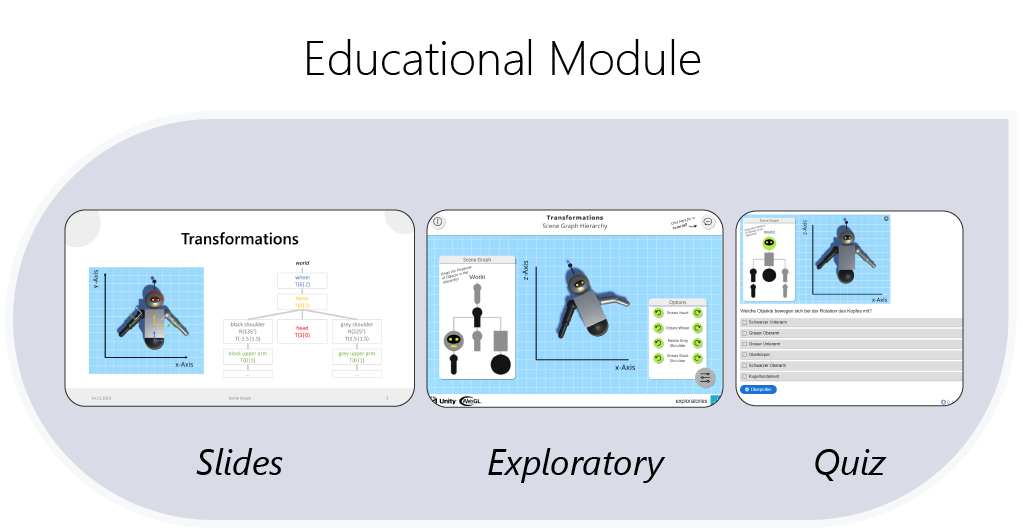
\includegraphics[width=\linewidth]{pictures/ExGoerContents.png}
	\captionsetup{labelfont=bf,textfont=it}
	\caption{Each of our educational modules consists of an exploratory, slides, and a quiz.\label{fig:contents}}
\end{figure}


\section{Related Work} %Fabian Pueschel
To facilitate the learning of CG for students, the intrinsically visual subject areas of CG were recognized as early as 1999~\cite{Balreira:2017:topics-cg-teaching}, and the resulting recommendations for interactive CG learning applications were highlighted. These have recently been the subject of several scientific publications, and the resulting learning applications can be categorized into programming-based and conceptual approaches:

\textbf{Programming-based approaches}, utilize code or parameters to visually modify computer graphics themes. They can make use of software libraries like \emph{Three.js} or WebGL~\cite{angel:2017:interactive} or simplified programming environments~\cite{Sueyasu:2010:cg-tool},~\cite{Lobb:2016:cg-tool}. While Angel~\cite{angel:2017:interactive} uses \emph{Three.js} and WebGL to teach CG simultaneously with an awareness of web programming, tools like "Simplified Language for Graphics Programming" (SLGP) and "CodeRunnerGL" offer less complicated environments for teaching rendering and 3D animations using pseudo-code~\cite{Sueyasu:2010:cg-tool},~\cite{Lobb:2016:cg-tool}.

\textbf{Conceptual learning settings} usually concentrate on teaching complex topics either by conveying the fundamental ideas step-by-step or not at all. These belong to the category of \emph{top-down} teaching approaches, which have been used for instance, in computer graphics, to teach different camera systems and transformations without assuming or exploring complex principles of mathematics or programming. This approach to teaching computer graphics is increasingly common in the current literature~\cite{Suselo:2019:problems-cg-teaching}. It is demonstrated through the creation of applications for personalized learning or using existing software.

Using \textbf{established software solutions} such as Maya~\cite{maya:2024:software} or Blender~\cite{blender:2024:documentation} modeling software, the software's internal functionalities are used to explain computer graphics concepts such as transformations, object creation, and animation~\cite{Elyan:2012:cg-tool},~\cite{Kadam:2013:cg-tool}. With this method, students can learn the functions and controls of the program while also comprehending three-dimensional representations more easily~\cite{Kadam:2013:cg-tool}. This enables students to understand the program more quickly while also understanding the notion of CG in three dimensions. However, the teaching content is restricted to the built-in features of the program being used, and it can only be marginally modified to fit particular teaching methods. For this reason, it may be necessary to create dedicated learning apps to teach more specific subjects. Thus, the scientific literature on teaching particular CG material frequently concentrates on the \textbf{creation of conceptual learning programs}, which can be downloaded or run locally on a desktop computer, or mobile, for instance, augmented reality (AR) apps.
Although there are apparent advantages of AR in education~\cite{wu:2013:current}\cite{lilligreen:2019:AWI}\cite{lilligreen:2019:EuroVR}, AR apps usually require mandatory installation~\cite{Qiao:2019:disadvantage-of-ar}, which makes consistent use during CG lessons difficult. However, when implemented as a platform-independent web application, the advantage arises that all students have constant access to the latest version of the application and it can be opened through a variety of output media without the need for installation~\cite{Eisemann:2023:cg-tool},~\cite{angel:2017:interactive}.  This is one of the reasons why our educational modules contain interactive web applications for the \emph {experiential learning} aspect.


Despite the variety of learning environments, the resulting learning platforms share many similarities in their forms of \textbf{interaction and topics}. To facilitate comprehension of complex CG concepts without engaging in the theoretical basics, the complexity is often reduced by using predefined interfaces in the spirit of \emph{conceptual learning settings}. In addition to predefined interfaces, our educational modules go a step further and strive to not only provide consistent ways of interactions across different topics but also to have a consistent look and feel. For this purpose, all modules are built using the same foundational framework of templates developed throughout the work of our study.

Predefined interfaces are frequently used to reduce complexity in computer graphics (CG) concepts so that they can be comprehended more easily without requiring an in-depth knowledge of theory. The "Graphic Teaching Tool" by Spalter and Tenneson~\cite{Spalter:2006:cg-tool} focuses on parameter-based modification of scenes and their visual representation. It adapts different graphics pipelines and their special features, such as transformations, and visualizes the resulting matrices using the example of the local desktop application. Further research has focused on different visualization and interaction approaches for teaching ray tracing processes~\cite{Suselo:2018:cg-tool},~\cite{ Verschoore-de-la-Houssaije:2022:cg-tool}, as well as the rendering pipeline, camera movements, and shadow mapping~\cite{Eisemann:2023:cg-tool}. Some of these topics are also covered by our set of OER modules (see~\autoref{sec:topics}) and the remaining can be easily developed based on the presented foundational framework.

There is a growing body of literature regarding \textbf{Open Educational Resources (OER)} as presented by Wiley et al.~\cite{wiley:2014:oer}. Regarding CG, the Computer Graphics Educational Materials Source (CGEMS) as described in Figueiredo et al.~\cite{figueiredo:2003:cgems}, \cite{figueiredo:2004:cgems2} as well as Anderson et al.~\cite{anderson:2017:NewCGEMS}, of the ACM SIGGRAPH Education Committee and Eurographics Education Board offer educational CG materials licensed under Creative Commons. Additionally, Ridge and Terzopolos~\cite{ridge:2019:ecosystem} introduced an online encyclopedia for computer graphics resources. Much like our work, it conveys different aspects of learning and combines them in a repository. Furthermore, it is possible to view some real-time animation examples within the encyclopedia. Like Wikipedia, it is to be seen rather as a work of reference. However, our education modules are specifically created with teaching CG in mind as a consistent package of ready-to-use materials. %https://github.com/encyclopedia-of-code/tiny-graphics-js
%https://www.realtimerendering.com/basics3js


\section{OER - Terminology and Challenges \label{sec:challenges}} %Florian Diller
As Wiley et al.~\cite{wiley:2014:oer} stated, there are a variety of definitions for the term OER. In our work, we refer to the \emph{Paris Declaration} of 2012~\cite{declaration:2012:paris}, which uses the definition of the term from UNESCO’s 2002 Forum on Open Courseware.

Atkins et al.~\cite{atkins:2007:review} already pointed out several challenges for OER to overcome in 2007, which were revisited seven years later by Wiley et al.~\cite{wiley:2014:oer}. In 2021  Tlili et al.~\cite{tlili:2021:towards} name the following challenges that OER face:
\begin{itemize}
	\vspace{-0.3cm}\item Lack of innovative teaching strategies
	\vspace{-0.3cm}\item Difficulty in monitoring the learning process
	\vspace{-0.3cm}\item Searching and locating OER
	\vspace{-0.3cm}\item Mapping OER together
	\vspace{-0.3cm}\item Feedback
	\vspace{-0.3cm}\item Adaptive learning
	\vspace{-0.3cm}\item Protecting intellectual property
	\vspace{-0.3cm}\item Fraud prevention
\end{itemize}

While we do not intend to solve these issues with the chapter at hand, there are some aspects, that are linked to these challenges.

\section{Topics Overview\label{sec:topics}}
%Listing of all exploratories and SHORT description
As already mentioned before, we developed educational modules for 14 different CG topics. To give the readers an impression of the context for which we developed the foundational framework and holistic integration we list the realized modules in the following. We also provide a short description of the exploratory contents of each module.
\begin{enumerate}
	\vspace{-0.3cm}\item \textbf{Scene Graph:} Example scene with interactive scene graph hierarchy and interactive objects (visible in the middle of~\autoref{fig:contents})
	\vspace{-0.3cm}\item \textbf{Light Sources:} Scene with different variable light sources
	\vspace{-0.3cm}\item \textbf{DDA Line Drawing:} Educational game, where the user has to place pixels similarly to a line drawing algorithm (see \autoref{fig:uxEval}a)
	\vspace{-0.3cm}\item \textbf{Field of View:} Example scenes with interactive viewing frusta to see the impact of the parameters in real-time (see \autoref{fig:uxEval}b)
	\vspace{-0.3cm}\item \textbf{Occlusion Culling:} Interactive example of occlusion culling and frustum culling with an overview to visualize the appearing and disappearing of objects
	\vspace{-0.3cm}\item \textbf{Backface Culling:} Different scenes including an interactive camera, an object with color-coding of culled faces, as well as displayed calculation
	\vspace{-0.3cm}\item \textbf{Level of Detail:} Moving the camera replaces different objects with more or less detailed counterparts depending on distance
	\vspace{-0.3cm}\item \textbf{Shading:} Examples of different shading methods with a variable light source, level of detail, and reflections
	\vspace{-0.3cm}\item \textbf{Transformations:} Editable transformation matrix featuring highlighting regions responsible for  rotation, scaling, and translation, and an object visualizing the respective transformation
	\vspace{-0.3cm}\item \textbf{2D Curves:} Hermite and B{\'e}zier curves with interactive boundary conditions and displayed basis matrix
	\vspace{-0.3cm}\item \textbf{Rotation:} Successively executable breakdown of the rotation around an arbitrary axis with variable axis location and rotation angle (see \autoref{fig:uxEval}c)
	\vspace{-0.3cm}\item \textbf{Convolution:} Step-wise executable convolution with variable filter sizes and padding options
	\vspace{-0.3cm}\item \textbf{Subdivision:} Step-wise animated execution of several iterations of the Catmull-Clark subdivision in 2D and 3D
	\vspace{-0.3cm}\item \textbf{Mesh Simplification:} Animated example of a grid-based mesh simplification algorithm with clickable cells allowing to initiate specific simplification steps
\end{enumerate}
All modules are publicly available as described in~\autoref{sec:publication}.
\begin{figure}[b!th]
	\centering
	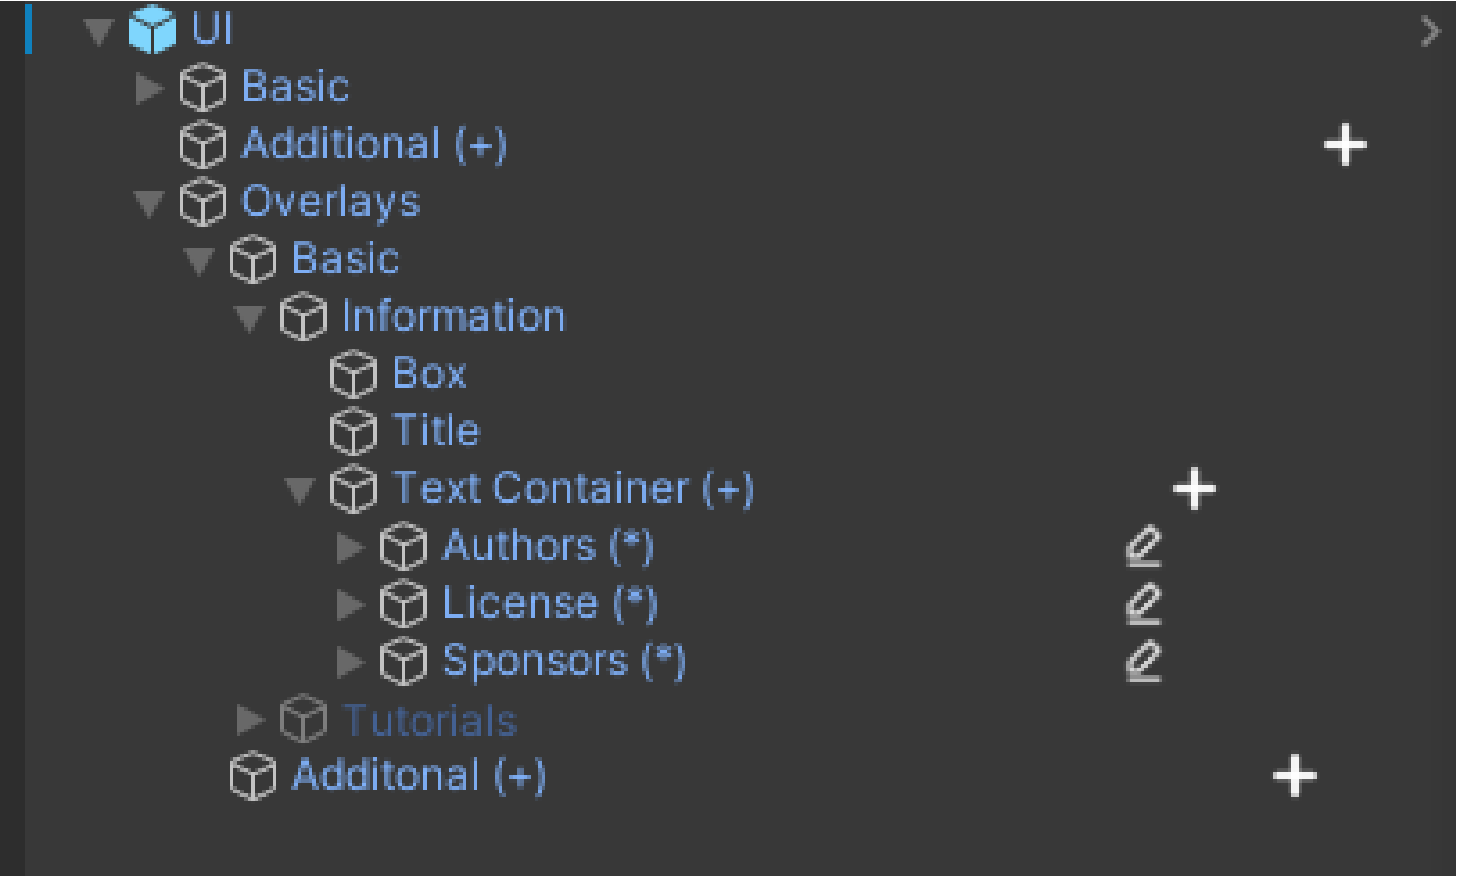
\includegraphics[width=\linewidth]{pictures/userGuidance_Icons.png}
	\captionsetup{labelfont=bf,textfont=it}
	\caption{The icons in the scene hierarchy let the user quickly identify possibilities to contribute. The \emph{pen} icon indicates editable objects, the \emph{plus} icon marks where new objects can be added.\label{fig:userGuidance}}
\end{figure}


\section{Holistic Approach}
In this section, we describe the details of the design and development of our educational modules. As mentioned before, they each include an application, presentation slides, and a quiz (see~\autoref{fig:contents}), and each of the modules is focused on a specific topic. Key features of the educational modules include consistency, modularity, and expandability to ensure a coherent and customizable learning and teaching experience. The following section systematically introduces these features, providing brief explanations of their relevance to our work, followed by a more detailed exploration in subsequent sub-sections, clarifying where these features manifest within the implementation, educational modules, in-app tasks, and challenges.

As a tool for the development of the exploratories, the game engine Unity~\cite{unity:2024:editor} has been chosen. Creating template scenes and templates objects (called \emph{prefabs} in Unity's terminology) for use with the game engine, we provide a modular framework that enables the creation of customized learning experiences through the seamless integration of pre-built components. In addition, various tools are made available to the user to facilitate the creation of personalized applications, supported by extensive documentation explaining technical aspects and guidelines.

\textbf{Consistency:}
Consistency serves as the backbone of our comprehensive approach, seamlessly linking all elements within our three-part modules. In the modules, including applications, presentations, and quizzes, uniform utilization of images, graphics, and textual content is used to facilitate a cohesive and integrated learning experience. The intuitive consistency promotes a holistic approach to understanding computer graphics and related areas, supporting a fluid and engaging learning journey.

\textbf{Modularity:}
Modularity is a foundational element in our approach, allowing the creation of independent, self-contained learning units. These units consist of modules encompassing an application, presentation slides, and a quiz. Furthermore, in the development of individual applications using our framework, multiple development templates can be employed. Yet, combined they form a rich learning experience. Each module stands on its own and allows students to focus on specific topics. This not only facilitates focused learning but also allows instructors to adapt and expand individual modules to meet the specific needs of their students, promoting flexibility and individualization.

\textbf{Expandability:}
Expandability is an essential part of our intention to create continuous improvement and adaptability. The following aspects establish easy expansion and updating: The open-source character of our OER combined with the modular approach in development, extensive documentation, annotation of the provided templates, the use of freely editable file formats (e.g. H5P~\cite{Singleton_Charlton_2019} for quizzes), and the use of a development environment (here game engine) in widespread use. This ensures that our content remains dynamic and offers educators the opportunity to improve existing modules or create new ones as technology and with it educational needs evolve. This adaptability contributes to the longevity and relevance of our educational resources.

\textbf{User Guidance:}
Icons (see~\autoref{fig:userGuidance}) and documentation in the provided templates make it clear where the resources can be used and adapted effectively. This user guidance is designed to help teachers and developers make changes exactly where they are needed without unnecessary complications. This guided tailoring of resources to individual needs increases the accessibility, usability, and overall effectiveness of our education system.
\begin{figure}[b]
	\centering
	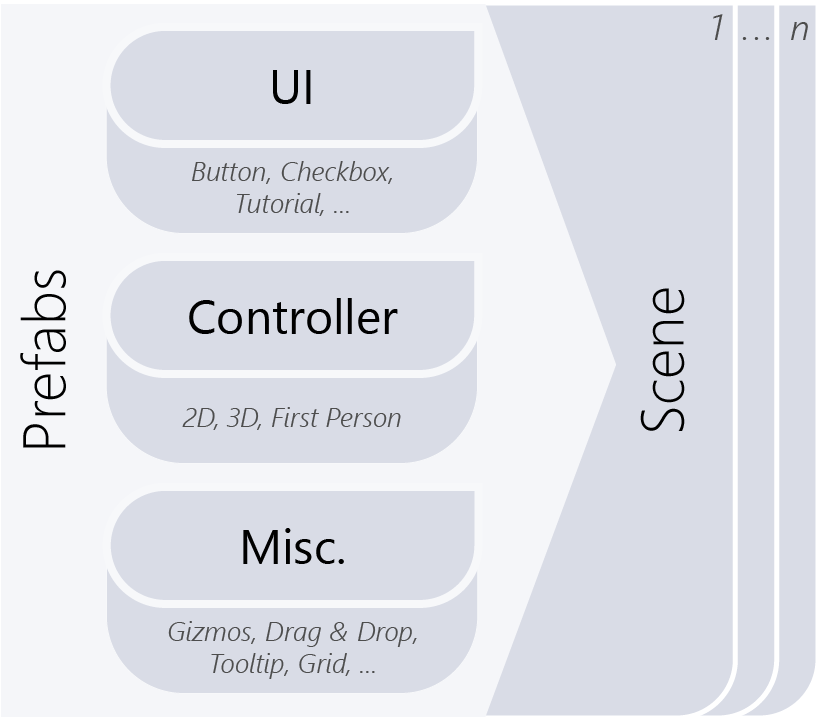
\includegraphics[width=\linewidth]{pictures/unityPrefabs.png}
	\captionsetup{labelfont=bf,textfont=it}
	\caption{Template objects (so-called \emph{prefabs}) enable the user to easily create customized scenes fit for their needs. \label{fig:unityPrefabs}}
\end{figure}
These key aspects collectively represent the concept of our overall design, which is not only technologically sophisticated but --- more importantly --- learning process-oriented. They form the backbone of an ecosystem where connectivity, adaptability, and accessibility come together to create a dynamic and enriching learning and teaching experience for students and teachers alike.
\begin{figure*}[t!bh]
	\centering
	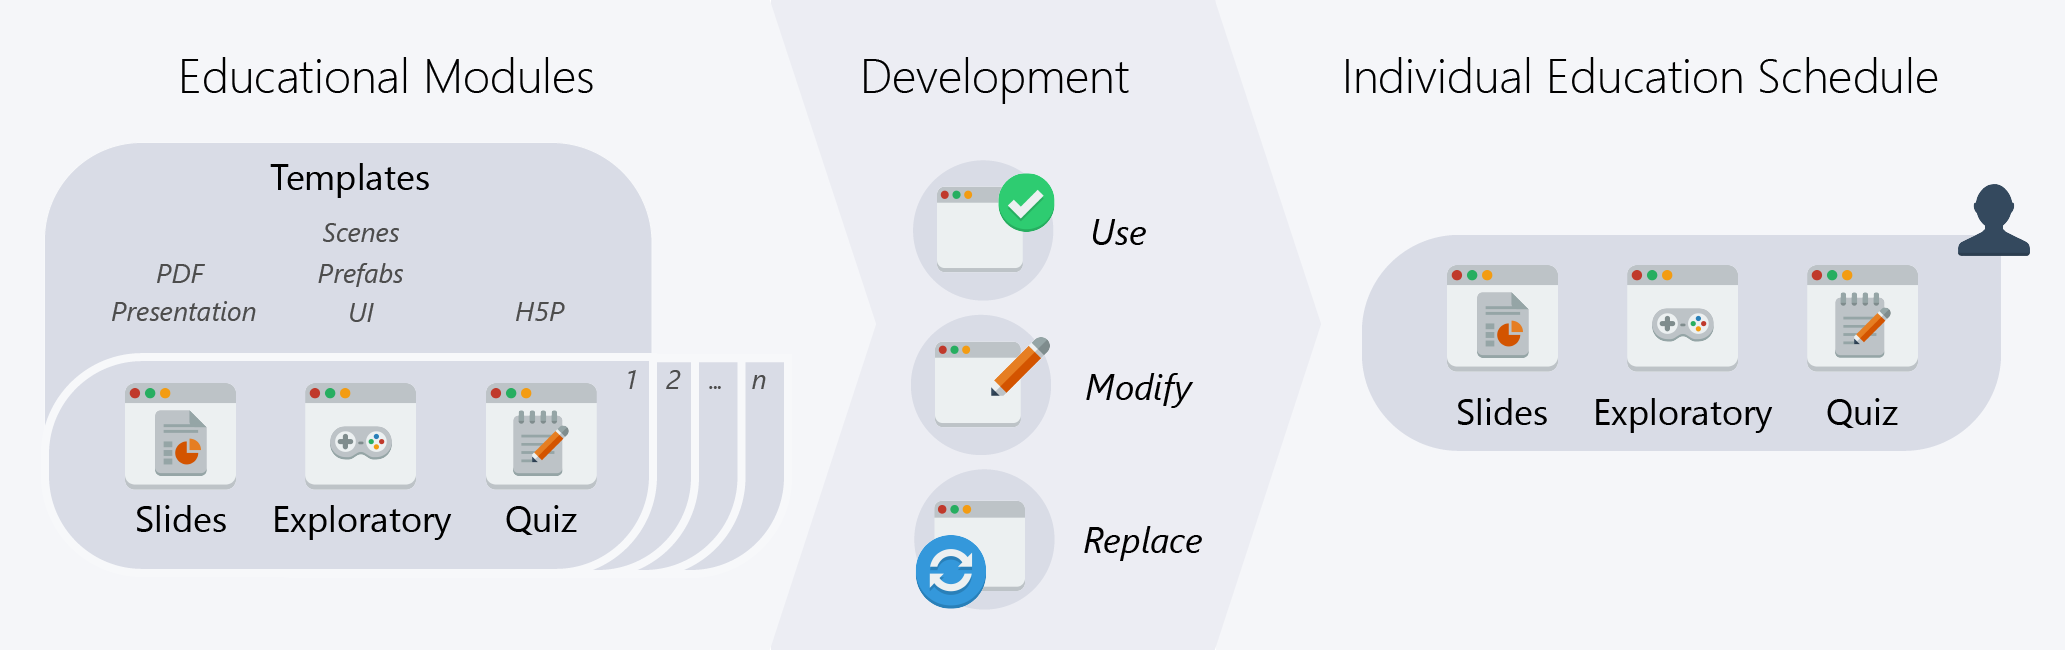
\includegraphics[width=\linewidth]{pictures/modularApproach.png}
	\captionsetup{labelfont=bf,textfont=it}
	\caption{Systematic overview of our educational approach and how to implement it in education schedules. We provide $n=14$ modules that are based on shared templates, which give them a consistent look and feel. By using the templates to create new modules, reusing or modifying existing modules, or replacing parts, other educators can create their own modules tailored to their individual teaching schedules.\label{fig:modularApproach}}
\end{figure*}
\subsection{Implementation}
%\textcolor{blue}{Modular., Expand, User Guidance (UI)} How do the above key points show in the implementation?

Our application comes with a framework of prefabs and scenes in the game engine Unity that follows a modular design approach. These components can be flexibly combined to create different applications within the educational package as visualized in \autoref{fig:unityPrefabs}. The provided Unity scenes are easy to use for certain control types. For example, developers can choose between a 2D or a 3D scene that is already equipped with the appropriate controls, user interface (UI), and camera. In addition, the provided prefabs make it easier to expand the UI by enabling the integration of useful elements such as buttons or tutorials. This modular structure not only increases the adaptability of the package but also facilitates the creation of customized educational experiences.
The pre-built UI is designed to support additional features to meet different educational needs. Users can easily expand the UI with features such as buttons and panels, providing a platform for the creation of advanced and customized learning applications.
Cues within the Unity framework, such as icons for editable or extensible components in the \emph{hierarchy}, provide clear visual guidance for user interaction (see~\autoref{fig:userGuidance}). These indicators, combined with detailed technical information presented in the comprehensive documentation, allow users, i.e. developers, to navigate the development environment with confidence.

\subsection{Educational Modules} %Teaching Bundles?
%\textcolor{blue}{Interconn., Modular (Folien,Quiz), Expand (Educational), User Guidance (Docu)} How does the above key points show in the framework?
The digital educational content has been carefully designed to flow seamlessly together and ensure a consistent visual identity. Each exploratory includes multiple recognizable graphical elements and details that reappear in the presentation slides and H5P quiz modules, creating a cohesive look and feel that enhances understanding of the topic. This can be seen, for example, in the screenshots of \autoref{fig:contents}.
The concept of modularity and expandability in our project is manifested through the deliberate design of multiple self-contained topics. Each learning unit operates as an independent module. This design allows for seamless integration and interchangeability of these units within an overall educational framework, e.g. in a lecture as visualized in \autoref{fig:modularApproach}. Whether educators wish to modify the sequence, introduce new content, or adapt existing modules, the modularity and expandability of our project allow them to do so effortlessly. This approach not only enhances the adaptability of the educational content but also facilitates a dynamic learning environment where each unit serves as a building block for teaching material fitting the educators' needs and a learning experience tailored to individual student groups. In addition, the widespread formats of the educational materials enable effortless integration within existing learning management systems (in our test scenarios, \emph{Moodle} and \emph{OLAT} were used) to deploy them among students and to evaluate the learning progress.

\subsection{In-App Tasks and Challenges}
%\textcolor{blue}{exploratories zum erkunden (FOV, Transform), gamification (DDA)}
In-app tasks serve as catalysts for active learning. These tasks are designed to motivate students to delve deeper into the subject matter and encourage them to apply theoretical concepts in a hands-on environment. By linking theoretical learning with practical tasks, we aim to promote a deeper understanding of the content. Another approach taken by us is inspired by gamification, bringing elements of competition and achievement into the learning process (see e.g. subfigure~\ref{fig:DDA}).
%The tasks in the app are designed not only as assessments but also as exciting challenges that transform the learning process into a quest for knowledge and insight.
This gamification approach not only increases motivation but also fosters a sense of accomplishment as students successfully complete each challenge. The integration of in-app tasks and challenges aligns seamlessly with our broader educational design philosophy. These challenges are intentionally chosen to align with specific learning modules, ensuring a direct connection between theoretical concepts presented in slides and applications and their practical use in the challenges. As students progress through the challenges, they not only reinforce their understanding of theoretical knowledge but also gain enthusiasm for exploration.

In summary, our holistic approach allows us to provide a cohesive, adaptable, and user-friendly learning experience. The incorporation of consistency, modularity, expandability, and user guidance forms a versatile foundation. Moreover, the integration of in-app tasks and challenges elevates the learning experience, turning it into an engaging process for both teachers and learners.

\captionsetup{labelfont={bf,color=black},textfont=it}
\begin{figure*}[t!b]
	\centering
	\subfloat[DDA Line Drawing\label{fig:DDA}]{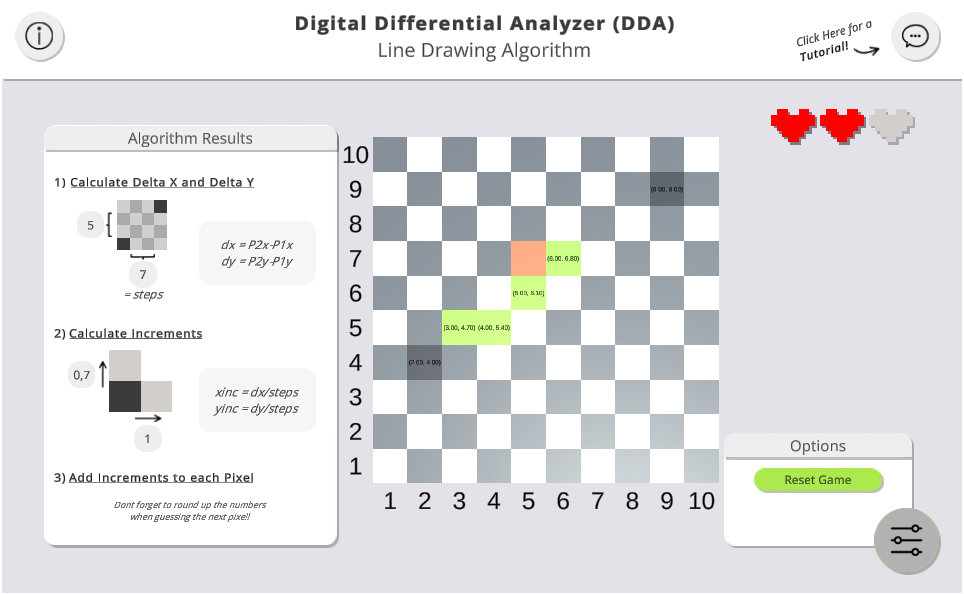
\includegraphics[width=0.33\linewidth]{pictures/DDAScreen.png}\hfill}
	\subfloat[Field of View]{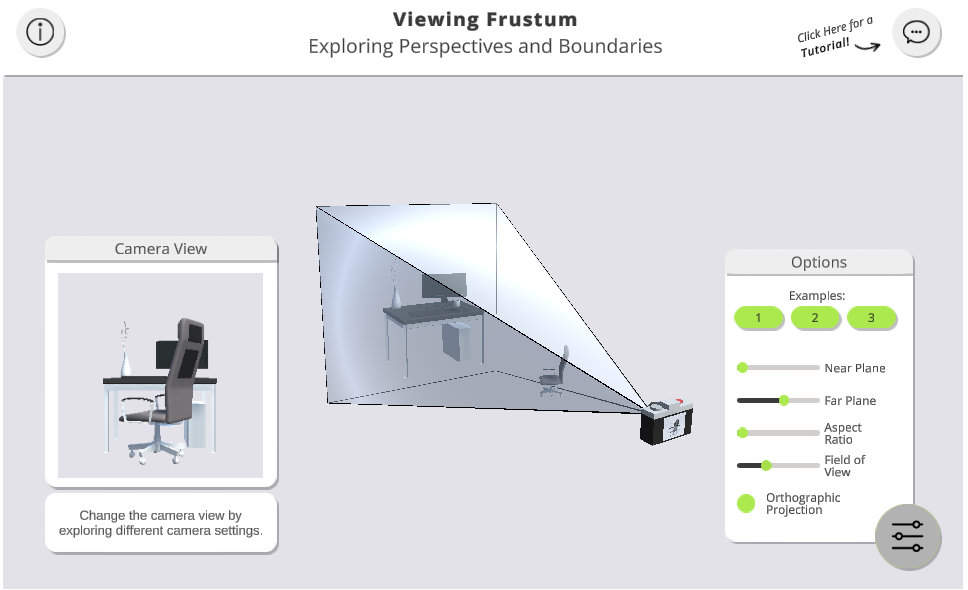
\includegraphics[width=0.33\linewidth]{pictures/fovScreen.png}\hfill}
	\subfloat[Rotation]{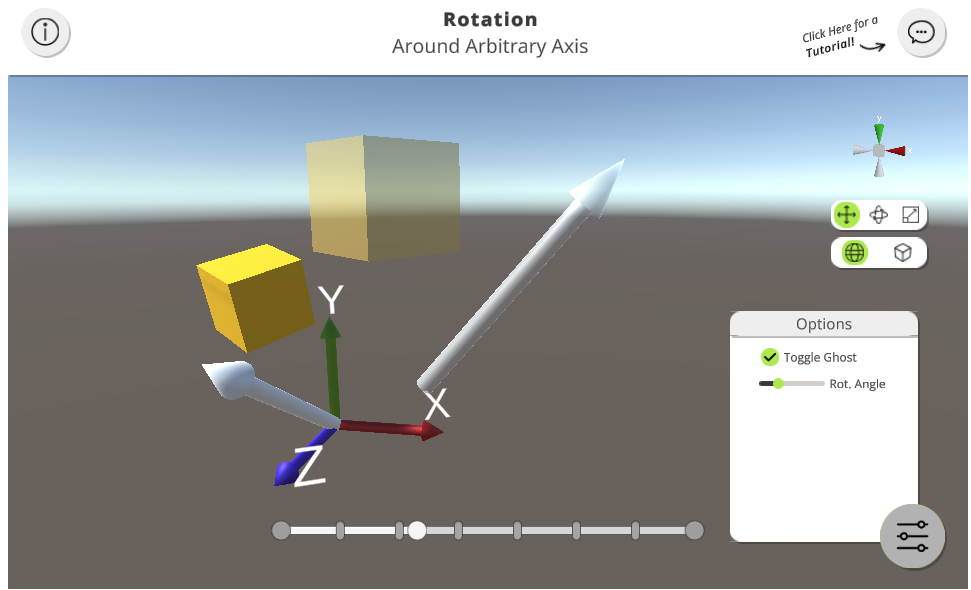
\includegraphics[width=0.33\linewidth]{pictures/RotationScreen.png}\hfill}
	\captionsetup{labelfont=bf,textfont=it}
	\caption{Screenshots of the selection of exploratories used to evaluate the UX of our modules. This should provide an overview of the contents and the design. The panels on the left provide additional information, and the panels on the right offer options to manipulate the scene.}
	\label{fig:uxEval}
\end{figure*}
\section{Publication\label{sec:publication}}
Our learning modules are available on the project website (\href{https://openedu-rlp.de/edu-sharing/components/collections?id=fd3957ef-80aa-4440-8956-c1d0d738c629}{https://www.openedu-rlp.de}). It includes the materials needed for forming individual learning schedules as seen in~\autoref{fig:modularApproach}. Additionally, there can be found the source files and documentation to use and build upon our materials, or create new exploratories. Furthermore, the materials can be found via other services, which refer to the project website. %The repository is publicly available at \url{https://gitlab.rlp.net/exgoer/exploratories.git}. 

\section{Evaluation}
%The integration of Open Educational Resources (OER) into education has earned increased attention in recent years, aligning with the ongoing trend of making educational content more open and accessible.
The following subsections describe the three different methods how we evaluated our newly developed overall concept and the specific educational modules. The aim is not only to assess the effectiveness of this concept and the modules but also to examine its pedagogical significance and potential challenges for educators and learners alike. The first two subsections explore the expert knowledge of a small number of individuals, while the third subsection provides insights into the interaction with a larger number of learners.

\subsection{Teaching Staff Interviews}%Julian Stockemer
This subsection examines the willingness to use the concept and the impact of its integration on teaching practice. This survey, involving five participants, was conducted during a university event focused on OER. The participants were introduced to our teaching concept, had the opportunity to experience the exploratories \emph{Field of View}, \emph{Backface Culling}, and \emph{Light Sources}, and posed questions. Subsequently, they completed a questionnaire.
The purpose of the survey was to obtain feedback from both educators and external participants. The questionnaire began by asking about the current integration of external tools and openness to interactive teaching methods. Following this, participants evaluated the utility of the presented concept in teaching and expressed their willingness to incorporate it into their lectures. Additionally, their inclination to utilize the provided examples developed by us or adapt the template for their own instructional content was queried. If respondents encountered challenges in these aspects, they were encouraged to list them.

Our teaching concept is primarily aimed at teachers and students. Nonetheless, we sought input from external participants to identify possible perspectives outside the educational community. Among the participants, three out of five were active in teaching. Four of five participants expressed a readiness to adapt their methods, with most of them integrating external content regularly. The unanimous desire for more interactive elements underscores their perceived pedagogical value.
In addition, another four of five participants were open to adopting the presented teaching concept, though half noted a need for additional skills for effective implementation. Despite this, all participants agreed on the content's accessibility and its meaningful contribution to student learning.
In summary, educators showed a positive inclination toward integrating interactive elements, with openness to the presented concept. The unanimous consensus on the accessibility of content provides a promising basis for the widespread adaption and adoption of the OER modules we presented.


\subsection{UX-Design Expert} %Florian Diller
To ensure the quality of our work concerning usability, a selection of three exploratories (\emph{DDA Line Drawing}, \emph{Field of View}, and \emph{Rotation}) as seen in~\autoref{fig:uxEval} with the corresponding slides was given to a UX design expert. Subsequently, a questionnaire with different statements was answered. Its results will be presented in the following.

The UI was predominantly good to use with no inconsistencies. Furthermore, it seemed to the expert that most users would quickly learn to handle the educational modules. The modules seemed rather straightforward and the integration of various functions in the system appeared successful. However, the navigation through the application would profit from a more detailed explanation. Especially one exploratory stood out, which was difficult to understand without the proper inclusion in a lecture. Although applications themselves feature a tutorial, they are intended to be included in a lecture and properly introduced by an instructor, which we were not able to provide to the UX-design expert. %Nevertheless, we see the module in question as a chance for further improvement.

The overall impression of our educational modules was highly attractive to the UX design expert.

\subsection{Students} % Florian Diller
We evaluated our experiential approach in practice by implementing eight exploratories in lectures. The selection consisted of the topics \textit{Transformation}, \textit{Rotation}, \textit{Scene Graph}, \textit{Shading}, \textit{Light Sources}, \textit{2D Curves}, \textit{Subdivision}, and \textit{Mesh Simplification}. The students took part in the experiments voluntarily.

To evaluate our approach among students, we applied split testing involving 19 individuals. Both randomized groups listened to a lecture regarding the educational content at hand. Subsequently, a quiz was taken by each participant. Then one group repeated the content with the conventional learning method of reviewing the script of the lecture heard. The other group followed the experiential approach and worked with the exploratory. Finally, both groups took the same quiz again and we recorded the increase of correct answers. Thus we were able to assess if the use of our exploratories leads to a larger improvement than conventional repetition methods. Overall, the improvement was evaluated 79 times across different exploratories. In our study, instructors did not explain the exploratories to the students in order to make the results of the study independent of the influence of individual instructors. The educational effect of the exploratories, however, could be improved by the instructor introducing the exploratories in detail.

The group of students using the exploratories showed a slightly higher improvement in test scores, 18~\% on average, than the group using conventional slide reading, which improved by 11~\% on average. When looking at the results, we see that some participants scored 100~\% in the first and second try, which leads to an improvement of 0~\%. Because these participants did not have the chance to improve at all, we could ignore them to get a clearer understanding of the improvement. Doing so, we see an average improvement of 25~\% in the group with the exploratories compared to 17~\% improvement in the group with slides. However, by conducting a one-tailed t-test with \(\ \alpha=0.05\), we see no statistical significance, considering the p-values of \(p=0.2>\alpha\) and \(p=0.16>\alpha\) with the data cleaned like explained above.
Nevertheless, the students responded exclusively positively to the exploratories and quizzes when conducting the experiments. For instance, the students requested permanent access to the exploratories and quizzes to support their studies. Furthermore, students expressed that the exploratories helped them understand the subject better, as the exploratories showed a different approach to it and let them experience the learning contents.

%possibly add "insights/discussion" section

\section{Conclusion} %Florian Diller
As the amount of OER is constantly growing, accessibility and fairness of education are raised. Consequently, education is made available to an increasing number of people from various cultures and backgrounds.

In this chapter, we presented a novel holistic modular approach to OER. We developed educational modules for 14 CG topics and published them as well as evaluated them with various user groups. The responses were positive throughout. While the evaluation of exploratory impact showed no statistical significance, a positive tendency was visible. The opinions we gathered from students, educators, and professionals showed that the use, development, and teaching of our OER modules appealed to them.

As mentioned in~\autoref{sec:challenges}, the challenges OER face are a topic, which is regularly revisited. Tlili et al.~\cite{tlili:2021:towards} mention several. Our work might represent a first step in solving some of them. The \emph{lack of innovative teaching strategies}, for instance, is addressed by the holistic experiential learning approach of our three-part education modules. The use of quizzes and exploratories activates the students and introduces variety to classrooms and lecture halls. Furthermore, the quizzes make it easier to \emph{monitor the learning process} and the platform on which we published our work allows for referencing from other websites, which simplifies \emph{searching and locating OER}.



\section{Future Work}
Although the chapter at hand showed a comprehensive way to develop, publish, and use OER packages, there are still desirable developments for the future. For instance, the framework we created will be used as a base to expand the existing topics and broaden the variety of exploratories and materials. Furthermore, the game engine we employed to develop the framework and the exploratories presented in this chapter is free of charge in certain situations (e.g. OER), but we intend to migrate the application framework to an open-source game engine like Godot (\url{https://godotengine.org/}) because it lines up even further with the ideas of OER to use open-source software to develop and access our materials. Additionally, our approach represents a good foundation for implementing \emph{microcredentials}. Following this approach, smaller educational topics are formally certified. This might raise the relevance of the project even further, make it possible to interlink it with other educational programs, and provide verifiability. Lastly, the impact of our work should be further assessed to a statistical significance. Consequently, we plan on conducting a more extensive user study.

\chapter{Visual Cue Based Corrective Feedback for Motor Skill Training in Mixed Reality: A Survey\label{chap:visualCueSurvey}}

Physical activity, especially exercise and physiotherapy, is important to improve and retain a healthy condition. In recent years, instructions and feedback given to learn and execute the relevant body movements have been increasingly supported by technology. In particular, systems employing mixed and augmented reality have been devised to support this so-called \emph{motor skill training}. The mixed and augmented reality technologies represent a platform for innovative new visualization techniques regarding motor skill training which are worth exploring.

In this chapter, we survey such approaches of visual feedback using mixed reality in the field of physical therapy, exercise and motor skill learning in general regarding the different visual feedback and technologies involved. In comparison to the existing surveys (see \autoref{sec:relatedwork}), we look deeper into which visual cues are used and how they are employed to achieve the goal of movement correction. To achieve this aim, we devise a classification of the approaches surveyed which involves, among other aspects, the used MR technologies, temporal and spatial characteristics of the feedback given, and the body parts addressed by the feedback. Additionally, we relate the approaches to stages of the way humans learn skills~\cite{fitts1967HPe}. The intention is to obtain a clearer view of which visualization techniques and visual cues are suitable for given tasks and to show where there are gaps in the existing research. The former can help practitioners and developers choose the appropriate visual cues for their task and system, while the latter can show researchers avenues for future research. 

This survey discusses approaches from 39 papers which were selected
out of 131 papers initially reviewed. These approaches were found to be relevant in terms of providing insight into the types of corrective visual motion feedback investigated in current research.

The focus of our analysis is aimed at the visual feedback of the surveyed literature. This does not include the therapeutic and medical aspects. We listed surveys addressing these points in \autoref{sec:relatedwork}.

\begin{figure*}[tb]
    \centering
    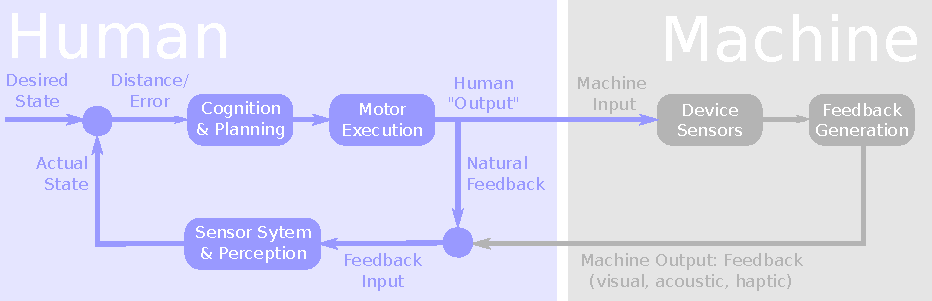
\includegraphics[width=1\linewidth]{pictures/feedbackloop.pdf}
    \caption{Illustration of the human-machine feedback loop based on~\cite{morone2021dab}\label{fig:feedback}. The \emph{machine} or \emph{system} usually is a computer with some kind of display, for example an augmented reality headset.}
\end{figure*}

\subsection{Related Work\label{sec:relatedwork}}
There is a limited number of surveys discussing visual feedback in mixed reality. While their scope regarding use cases, body parts, or technologies is often narrower than ours, the analysis regarding the types of feedback and the forms it can take is broader. The survey at hand goes in more depth regarding feedback while retaining a wide scope of use cases, body parts, and technologies. In the following paragraph, we will discuss related surveys and ways in which our work complements the existing research.

The scope of the present work, and therefore the scope of the related surveys, is located at an intersection between medicine, sports, and computer science. In the medical literature, surveys like Mubin et al.~\cite{mubin2020esg}, Schiza et al.~\cite{schiza2019vra}, Gandhi et al.~\cite{gandhi2020mts} and Rutowski et al.~\cite{rutkowski2020uvr} provide a treatment-oriented perspective on the field of digital feedback for movements. Their overview and analysis are mainly focused on the outcome of the treatment and less so on the type of visual feedback. The chapter at hand however is concerned with the visualization of the feedback given. Related surveys from the \emph{physical exercise} part of the literature, in particular, Perin et al.~\cite{perin2018sas} and Liebermann et al.~\cite{liebermann2002aai}, look at the performance regarding exercise.
One topic connected to visual feedback is (serious) gaming. Thus, it is worth noting that the above-mentioned Mubin et al. \cite{mubin2020esg} and Ma et al.~\cite{ma2011vrp} discuss serious games in health care. Sawan et al.~\cite{Sawan2016MRS} present a literature review on how various MR and AR technologies are used in the sports industry. The review provides insights on the sport-related use cases of MR and AR technologies.

Gatullo et al.\cite{gatullo2020whw} conducted a systematic literature review and classification for visual assets in industrial augmented reality applications. As skill learning and training are an important use case for augmented reality in the industrial context, their work is related to ours. The focus of their approach, however, lies heavily on tool handling, which we excluded from the scope of this work (see~\autoref{sec:tvcg:methodology}).

In addition to these generally related publications, there are a few papers that stand out as being closer to our approach, as they analyze visual aspects of feedback and hence have a scope overlapping ours:

Viglialoro et al.~\cite{viglialoro2019rar} investigate literature aiming at \emph{shoulder rehabilitation} supported by augmented reality. The scope of their review led to a sample collection of nine papers. The arm and hand movements of the users, as well as rehab settings, target groups, tracking technologies of each augmented reality (AR) system, user interfaces, and evaluation methods, were investigated.

The work of Neumann et al.~\cite{neumann2018sra} surveys 20 approaches focusing on \emph {virtual reality} in physical exercise. They investigated activity, equipment, virtual reality (VR) technology, point of view, and whether other persons than the user are present in the environment. The characteristics of test groups were looked at as well. The number of participants, gender, age range, experience type, and location were investigated and documented. Additionally, the paper summarized the aims, conditions, measured features, immersion, and key findings of the researched literature.

Brennan et al.~\cite{brennan2019fdt} analyzed literature about feedback design in \emph{home rehabilitation}. While this comes close to our approach, they did not focus on mixed reality and limited their scope to home rehabilitation, which resulted in a smaller body of literature of only 19 research attempts. Clinical context, system components, feedback design, and the evaluation of these features were investigated. The feedback characteristics were categorized and analyzed. This resembles our approach, although we took a closer look at the visualizations \emph{per se}. The smaller scope of our survey in comparison to the approach of Brennan et~al. enabled us to analyze visual cues in more detail.


\subsection{Organization of this Chapter}
This chapter starts with an introduction establishing the motivation of the present survey and relating it to previous works as well as putting it in scientific context. Relevant terminology and fundamental concepts like feedback and skill learning basics are introduced in \autoref{sec:background}. In \autoref{sec:tvcg:methodology} our methodological approach to acquiring literature is explained and the guidelines we followed to do so are described. \autoref{sec:classification} elaborates on how we categorized the literature and the features we chose for that matter. \autoref{table:2} shows the results of our classification and represents a central point of reference for the whole chapter. To make the nature of the surveyed literature more accessible to the reader, an exemplary discussion can be found in \autoref{sec:exemplary}. In \autoref{sec:tvcg:insights} the main insights of this survey are presented. The chapter is concluded by summarizing the findings, mentioning limitations, and highlighting interesting open questions in \autoref{sec:tvcg:conclusion}.


\section{Background and Terminology \label{sec:background}}
To establish a common ground for understanding and discussion, we explain the definitions of the most important terms in this section. Additionally, we provide an overview of the fundamental concepts we are working on in this chapter.

\subsection{Feedback \label{sec:feedback}}
The term \emph{feedback} originates from electronics as stated by Morone et al. \cite{morone2021dab}. In this context, the output of a system is combined with the input to affect the function of the system. This idea was later transferred to the social sciences, as humans observe their \emph{actual state} and regulate their behavior according to a \emph{desired state} to minimize an \emph{error} (or \emph{distance} in our case), as stated by Morone et al.~\cite{morone2021dab}. This idea is illustrated in \autoref{fig:feedback}. The \emph{natural feedback} loop, which is represented on the left in \autoref{fig:feedback}, involves planning, executing, perceiving, and adjusting the movement.


This feedback loop can be extended to incorporate a technical feedback system as seen in the literature we analyze (represented by the right loop in \autoref{fig:feedback}). To provide feedback, the machine detects certain aspects of the human output (in our case the movement). This information then enters the system as \emph{machine input} via \emph{device sensors}. The machine-\emph{generated feedback} is then delivered to the human as a (in our case visual) \emph{machine output}.

The scope of the present chapter includes literature which for the most part includes what Morone et al.~\cite{morone2021dab} define as 'augmented feedback'. This means the user is already aware of the feedback signal given by the system. In our case, the visual information of the body position in space is emphasized by the feedback, and a focus is placed on movements that the users can readily detect themselves.

The term \emph{augmented feedback} has to be distinguished from the term \emph{biofeedback}, which is commonly used in current literature. It often occurs in the context of device-supported rehabilitation feedback. When used accordingly, it refers only to signals the users are not aware of, for example in electromyography (EMG), where the electrical activity of the muscle is measured \cite{mills2005bem}.

In educational settings, feedback is traditionally given by another person, usually a teacher, instructor, or trainer (see \autoref{sec:instructor}). In this context, feedback that enables participants to correct their behavior is often called \emph{corrective feedback}~\cite{hattie:2007:Feedback,Lysakowski:1982:Feedback}. Similarly, in a feedback system, information qualifies as corrective feedback if it gives the user insight into how the movement can be carried out differently in order to accomplish the task at hand correctly or at least in an improved manner. 

To be precise at this point, it has to be mentioned that in computer science 'feedback' is often used for the response of a system to confirm input by the user~\cite{ADictionaryofComputerScience}. This meaning of the term is not relevant to the scope of this chapter.

\subsection{Phases of Skill Learning in Physical Activity\label{sec:stages}}
The acquisition of new skills proceeds in three stages or phases as described by Fitts and Posner~\cite{fitts1967HPe}. These phases of skill learning are connected to motor skill acquirement as shown by various authors (see e.g. \cite{schmidt2004motor,SWINNEN1997749,SINGER197879} and \cite{taylor2012rsm}). The three stages as seen in \autoref{table:1} successively take place one after another over the course of internalizing a movement.

Skill acquisition starts in the \emph{cognitive} stage, where the learner tries to grasp the overall concept and understand what to do. The flow of information from an instructor (or instructions) to the learner plays a major role during this phase, as the learner still processes what to do. 
In the \emph{associative} stage the learner will construct the actions to be done from minor movements (subroutines) and the information gathered during the cognitive stage.
The final stage is the \emph{autonomous} stage. Herein the learner has fully internalized the movement. The cognitive capacity needed for the movement is minimal in this stage. Thus, additional information can be accessed or processed while making use of the skill. The efficiency and performance of the activity enacted still increase in this stage.

Once the learners have internalized an action, they can revisit stages to improve and 'relearn' their movements~\cite{huber2013AEP}. As stated by Fitts and Posner~\cite{fitts1967HPe} the transitions between stages are not always clear. Nevertheless, it will be useful in the survey at hand to relate the skill level of the target group to the feedback given.

\begin{table}[ht]
\caption{Fitts and Posners~\cite{fitts1967HPe} stages of skill learning as applied to motor learning. Presentation based on~\cite{huber2013AEP}.\label{table:1}}
\begin{tabular}{ |p{2.2cm}||p{2.6cm}|p{5.2cm}|p{2.2cm}|  }
    
 \hline
 Stage & Process & Characteristics & Other name\\
 \hline
 \hline
 Cognitive & \raggedright Gathering Information & \raggedright Large gains, inconsistent performance & Verbal-motor stage \\
 \hline
 Associative & \raggedright  Putting actions together & \raggedright Small gains, disjointed performance, conscious effort & Motor stage \\
 \hline
 Autonomous & Much time and practice & Performance seems unconscious, automatic and smooth & Automatic stage \\
 \hline
\end{tabular}
\label{table:stages}
\end{table}

\subsection{Instructor or Agent\label{sec:instructor}}
In Fitts and Posner's work~\cite{fitts1967HPe} discussed above, instructors play a central role. They transfer knowledge to the learner and decide what input is suitable at a given moment. In most mixed reality systems, a machine substitutes the instructor as illustrated in \autoref{fig:feedback}. This means that feedback systems have to be designed carefully with the user in mind (participatory design)~\cite{davies2003vrf}. Oftentimes health care professionals are included in this process~\cite{hilton2011dem}.

Hattie and Timperley establish the more general notion of an \emph{agent} in their work~\cite{hattie:2007:Feedback}. This notion includes teachers, peers, books, parents, the self, and experience. It can be regarded as analogical to the term instructor. A mixed reality system substituting the human instructor qualifies as such an agent. Virtual Trainers, virtual medical professionals, and simplified human shapes are depicted in mixed reality to provide feedback to the user, to hint at positional discrepancies, or to show in advance what positions to copy. A good example for this is the work of Mostajeran et al.\cite{mostajeran2019hvc}, which utilizes a virtual coach offering instructions to the user.

A few systems included in our survey, like those described by Debarba et al.~\cite{debarba2018arv} and Furukawa et al.~\cite{furukawa2018dar}, provide feedback to instructors. These approaches are applied to rehabilitation but could also be applied to physical exercise or skill learning in general. One advantage of systems targeting instructors is the exact metrics they can provide to the instructors. Consequently, the instructor is well-informed and can decide what information to give to the learner or client.

\subsection{Immersion \label{sec:immersion}}
As discussed by Nilsson et al. \cite{Nilsson2016irr}, there are various definitions of immersion that seem to differ from one another quite considerably.
What they all seem to have in common is that immersion influences a feeling of \emph{presence}, an impression of being there. Ijsselsteijn et al. \cite{ijsselsteijn2004fas} established that immersion, and connected with it, presence help to motivate users. They even increase the feeling of competence and control, which is highly relevant when applying a given feedback and hence correcting a false movement.

\section{Methodology and Scope \label{sec:tvcg:methodology}}
To acquire literature for this survey, we conducted \emph{snowballing} as a search approach. The snowballing followed a scheme similar to the one described by Wohlin \cite{wohlin2014gss}. We preferred snowballing rather than database keyword searches because it has been shown to be more effective for acquiring sources in general (see \eg\ Greenhalgh et al. \cite{greenhalgh2005ees}, Badampudi et al. \cite{badampudi2015eus}). As \emph{start set} for the snowballing, we used the papers mentioned in related works (\autoref{sec:relatedwork}). While snowballing, we did not limit ourselves to papers, but included all sources of interest to the research community, considering all sources which incorporate motor skill training in mixed reality.

To decide which of the papers obtained to include in the survey, we conducted a screening analogical to the flow diagram of the PRISMA (Preferred Reporting Items for Systematic Reviews and Meta-Analyses) guidelines described by Liberati et al. \cite{liberati2009prisma}.

Since the field of mixed reality is moving fast and there have been major changes and innovations in recent years, we additionally limited the publications to be surveyed to those which have been published in the period since 2016. The year 2016 marks the launch of Microsoft's AR headset \emph{HoloLens} which represents an important development to the research community in the field of mixed reality applications~\cite{Park2021}.

In detail, through snowballing with the above-mentioned scope, we identified 131 promising papers. After screening, we found 28 papers were not relevant to our overview, since their keywords or title might have sounded promising, but their content did not match our scope. Subsequently checking for eligibility according to the use of visual \emph{corrective feedback}, 64 more papers were excluded. We found that these papers did provide \emph{corrective feedback} in the sense explained in~\autoref{sec:feedback}. In the end, 39 papers matching our scope and providing suitable content were included in the review. The methodological quality of the papers has not been evaluated.

To verify our acquisition and selection process, we conducted a database search in \emph{Google Scholar}, \emph{IEEE Xplore} and \emph{ACM Digital Library} using search terms extracted from the literature matching our criteria. For this purpose, the word pairs with the highest occurrence among the paper titles (ignoring filling and linking words) were identified. Two pairs were each combined with \textit{AND}-arguments to a search term resulting in three or four words per term depending on duplicate words in the pairs. All databases were searched with the same terms. No additional relevant papers were found by this process. Thus, we conclude that the snowballing was effective and sufficiently thorough.

It appears to be especially important to mention why certain types of approaches are not as present in this survey. First, approaches that utilize movements only as an input (e.g. walking-in-place in VR applications) are not covered by this survey as they do not provide motion feedback (\emph{corrective feedback}) in the sense we discussed in \autoref{sec:feedback}. Input movements as seen in \emph{walking-in-place} approaches or even mouse clicks are merely necessary means to control systems and applications. Exertive movements as an input are usually used to increase immersion. 

Second, exergames~\cite{oh2010defining} or serious games are usually designed to fulfill certain objectives, like sports or rehabilitation. Corrective feedback as discussed in \autoref{sec:feedback} is provided in just a few instances, for example the papers by Afyouni et al.~\cite{afyouni2020arb}, Caserman et al.~\cite{caserman2021fbm}, Raffe et al. \cite{raffe2018cst} or Booth et al.~\cite{booth2019vue}. These works do not define their use of the term \emph{feedback}. But they provide a visual incentive to carry out a certain movement \emph{correctly}.

Third, mixed reality skill training occasionally focuses on handling tools. Examples of such approaches have been described by Pucihar et al.~\cite{pucihar2015dcm} and Mohr et al.~\cite{mohr2017rvt}. These approaches give feedback for motor skills but often focus on the tool itself, not on the body. Although for handling a tool a complex combination of body movements is necessary, and although the position of the tool is a result of these complex combinations, we still excluded papers with a missing focus on the body from the survey. Nevertheless, we included work that gives feedback for the body parts handling the tools. One such approach by Furukawa et al.\cite{furukawa2018dar} provides feedback for hand positioning while writing calligraphy. Another relevant approach regarding tool use is the work of Cao et al. \cite{cao2020esa}, who utilize augmented reality to show full body feedback for skill training involving machine tasks.

Fourth, there is at least one research attempt that appears noteworthy, although it predates 2016 and is thus not included in the main scope of this chapter: The approach of Tang et al.~\cite{tang2015pah} provides corrective feedback involving visual cues similar to many of the other references in the present survey. Thus, this work could be categorized according to~\autoref{sec:classification} without problems. What is especially interesting when considering this work are the similarities and differences of the used visual feedback categories \emph{movement arc}, \emph{directional arrow}, \emph{nearest arm}, and \emph{topdown angle} to the categories we use in \autoref{sec:classification}.


Finally, our intent is to investigate the visual cues related to movement feedback from a visualization standpoint. Thus, we do not analyze the therapeutic aspects of the surveyed approaches.

\section{Classification \label{sec:classification}}
To analyze the work surveyed in this chapter and to provide insights about it, we select different features and characteristics to classify and group the literature. The following paragraph outlines which categories were chosen, why they are important, and how they impact visual feedback. Each category is described in a separate subsection below and \autoref{table:2} depicts the complete conducted classification. The classification is directed at the visual computing aspects of the feedback. The therapeutic and medical aspects of the topic are discussed elsewhere (see \autoref{sec:relatedwork} for more information).


The \textit{technology} used to implement mixed reality has a big influence on immersion (see \autoref{sec:immersion}) and feedback visualization. Additionally, the \textit{point of view} is important to distinguish, as it influences the identification with the avatar as well as the immersion and therefore the impact of feedback. It also affects which body parts are visible to the user. The \textit{abstraction type} of the feedback determines what kind of information is provided to the user. It is possible to provide feedback at different times of the process. This \textit{temporal order} impacts the learning process and changes the way feedback is perceived. A classification into the former mentioned \textit{stages of learning} (see \autoref{sec:stages}), can give a quick indication of how and in what depth the system provides feedback. The type and the scope of feedback change drastically depending on the \textit{body parts} for which the feedback is provided and both, type and scope, are strongly connected to the \emph{use case} (sports, rehabilitation, etc.) the feedback is aimed at. Lastly, the \textit{publication venue} is a higher-level feature to classify the literature.

\subsection*{MR Technologies \label{sec:MR}}
There are different definitions regarding the term \emph{mixed reality}~(MR)~\cite{whatIsMR}. For this study, we based our definition on the reality-virtuality continuum of Milgram et al. \cite{milgram1994arc}.

The mixed reality \textit{technologies} used in the surveyed literature involve very diverse approaches~\cite{schmalstieg2016augmented}. Essentially HMDs for both VR and AR are widely spread. HMDs used in AR can be further categorized as \textit{optical see-through}, in which the real world is perceived through glasses and the virtual elements are added to it, and \textit{video see-through}, which shows virtual elements together with the camera-captured surroundings. A special implementation of VR is \textit{CAVE}, which combines life-sized screens with stereo glasses to create an immersive digital environment. In the context of AR a room-mounted \textit{display}, oftentimes displaying an augmented mirrored camera image (augmented mirror), can be used to provide feedback. Finally, there are AR approaches which augment the environment by \emph{projecting} computer graphics directly into it.

\subsection*{Point of View \label{sec:POV}}
The point of view (POV) plays an important part in the type of feedback that can be given. A \textit{third person} or \textit{exocentric} perspective (\autoref{fig:POV}, left) can provide a full-body view, which makes it easier to supply complete feedback for multi-joint movements and complex movement sequences.

It could be argued the immersion provided by a \textit{first person} or \textit{egocentric} point of view  (\autoref{fig:POV}, right) is superior to a third-person view. This would mean a first-person view offers more motivation and a feeling of control (see \autoref{sec:immersion}). However immersive HMDs often feature a limited field of view~\cite{trepkowski2019enf}, which can lessen the user's ability to see and correct position or movement for certain body areas. 

There are approaches that combine \textit{both} of the above-mentioned features.

\begin{figure}[b!th]
    \centering
    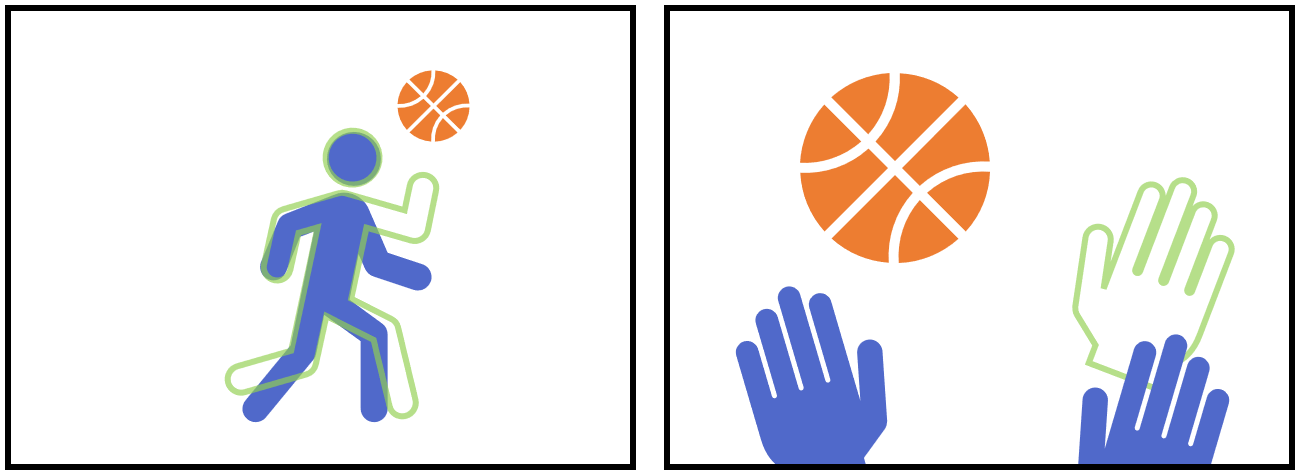
\includegraphics[width=\linewidth]{pictures/PointOfView.PNG}
    \caption{A person exercising with a ball. Exocentric (left) and egocentric (right) view types with possible target movement (feedback) in red and the actual movement in black.\label{fig:POV}}
\end{figure}


\subsection*{Abstraction Type}
The \textit{abstraction type} of movement information used for giving feedback impacts the users' experience and the corrections they execute. \textit{Directional feedback} shows the direction in which a limb should be corrected. For example, arrows can be utilized to achieve this. An alternative to showing the correcting movement is to visualize the target state. \textit{Positional feedback} predominantly does this with an outline, transparent target avatar, or end position to show where the ideal position is. In contrast to that, \textit{guidance} demonstrates the desired movement before the user will execute it. The concrete visual cues being used to provide these types of information are described in \autoref{sec:visualCues}.

\subsection*{Temporal Order}
The \textit{temporal order} in which the feedback is provided in the context of the movement execution varies in the analyzed approaches. In some cases, a \textit{playback}, where the feedback is shown after the execution, might increase the precision of movement, while in other cases a \textit{real time} feedback offers an instantaneous in-situ opportunity to apply correction. Additionally, it is possible to show the user the future movements, which can provide information about \textit{upcoming} target motions.

\subsection*{Stages of Learning}
Considering that motor feedback can help users learn a skill, Fitts and Posner's \cite{fitts1967HPe} stages of learning can be applied to visual motor feedback.
We use the feedback features provided by the surveyed literature to assign each approach to one of the \textit{stages of learning}. This assignment can provide useful information regarding which part of the learning process the feedback addresses and which depth it can provide. The stages are explained in more detail in \autoref{sec:stages}. It is also to be said, that the stages are transitioning into each other fluently and that in some cases arguments for a classification into a different category can be made \cite{fitts1967HPe}. 

\subsection*{Publication Venue}
The literature surveyed is sourced from several different \emph{publication venues}. We categorized the venues as \emph{computer science (VR, AR, MR)}, \textit{computer science (HCI)}, \emph{computer science (other)}, \emph{medicine, health \& sports} as well as \emph{patents}. These categories can give readers a general orientation in which areas most of the research is rooted and where there is still potential. The descriptions from authors from different venues also usually put emphasis on different parts of the respective approaches (e.\,g. application vs. technology vs. usefulness).

\subsection*{Body Parts}
Furthermore, the \textit{body parts} for which feedback is given are of interest. The feedback changes with the degrees of freedom of different joints. It is also interesting to consider how the visibility of a body part in a neutral position interacts with the feedback (see \autoref{sec:POV}). In the literature we surveyed, the feedback was provided for \textit{arms}, \textit{legs}, \textit{hands}, or the \textit{whole body}.

\begin{figure*}[tb]
    \centering
    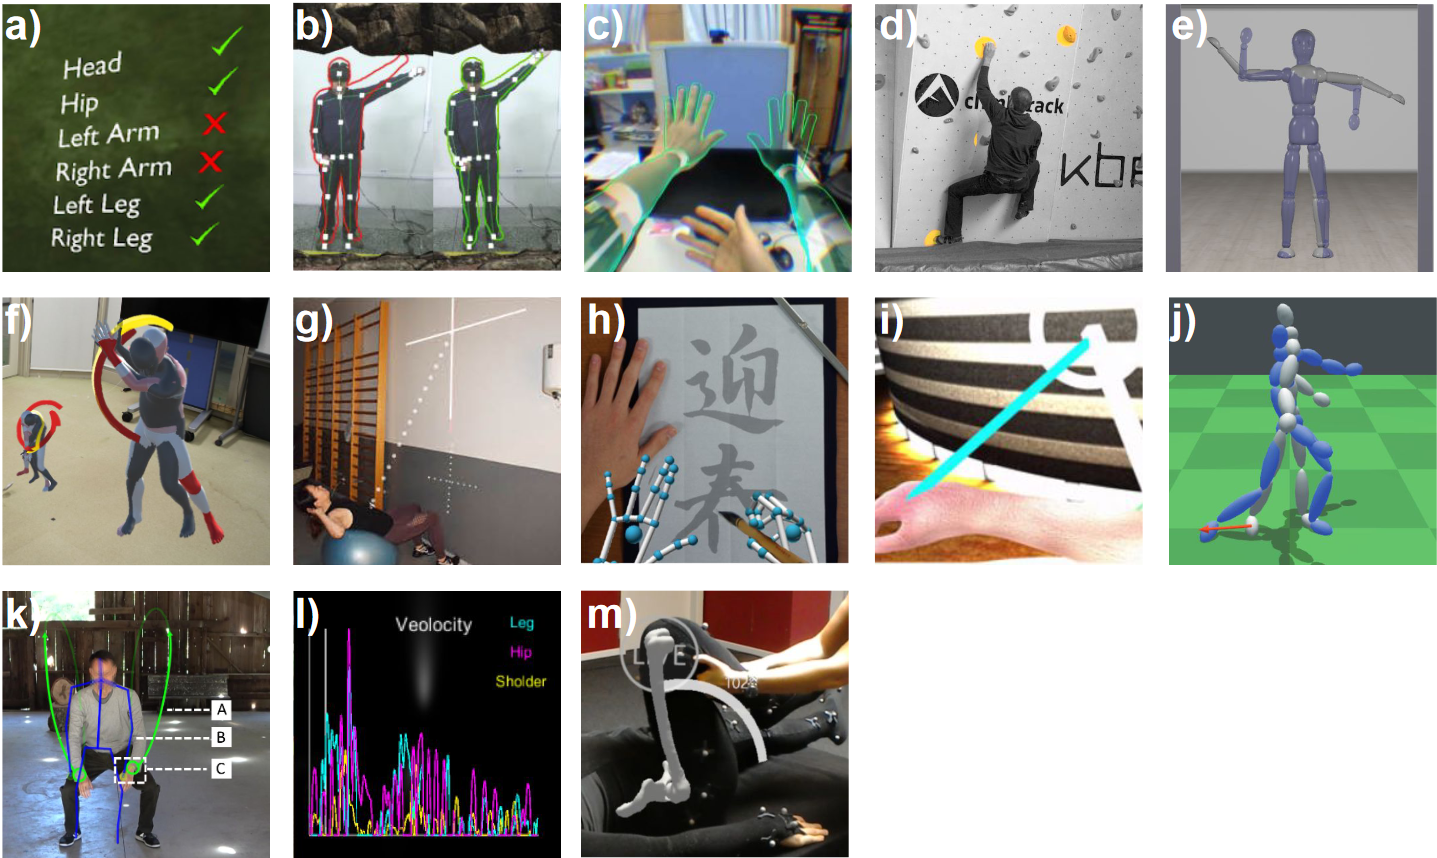
\includegraphics[width=1\linewidth]{pictures/CueMatrix.PNG}
    \caption{Examples of visual cues used in the literature and described in~\autoref{sec:visualCues}: a) Textual, b) Color coding, c) Body outline, d) End position, e) Transparent target avatar, f) Opaque target avatar, g) Abstraction, h) Video overlay, i) Rubber bands, j) Arrows, k) Trajectories, l) Graphs, m) Limb angles.  Images from \cite{caserman2021fbm},\cite{quevedo2017asr},\cite{han2016ara},\cite{wiehr2016bce},\cite{waltemate2016tlp},\cite{ikeda2018arb},\cite{vidal2020blo},\cite{furukawa2018dar},\cite{yu2020pmd},\cite{oshita2018sts},\cite{clarke2020rva},\cite{takahashi2019vrb},\cite{debarba2018arv}. \label{fig:CueMatrix}}
\end{figure*}

\subsection*{Use Case}
The analyzed approaches showed a wide variety of use cases the feedback was given for. We identified \textit{individual sports}, \textit{team sports}, \textit{rehabilitation}, and \textit{motor skill training} as typical use cases. \textit{Motor skill training}, here, does not only include approaches that analyzed motor skill training \emph{per se}, but also the ones that had no use case taken into consideration so far.


\subsection*{Visual Cues \label{sec:visualCues}}
The visualizations in the literature surveyed featured several different \textit{visual cues} to indicate how a target movement should be executed. These visual cues are the most in-depth description of the feedback we provide and are closely linked to other features such as technology, body parts, and use cases. The distribution of visual cues among the literature surveyed is listed in \autoref{table:2}. Exemplary images for all the visual cues explained in the following can be found in \autoref{fig:CueMatrix}. The labels of the examples in  \autoref{fig:CueMatrix} correspond to the letters found in front of the visual cue names in the following description.

\textbf{a) Textual}

Hints to correct the movement with words or text were categorized as \textit{textual}. These cues are in most cases combined with other feedback methods (\eg\ Oshita et al. \cite{oshita2018sts} and Conner and Poor \cite{conner2016cef}).

\textbf{b) Color Coding}

Colors can be an intuitive indicator of wrong or right (\eg\ red/green). For example an avatar with color-changing limbs or joints (as in \autoref{fig:Oka} taken from the work of Oka et al.~\cite{oka2021rtf}) can be used to give feedback for a desired movement. The \textit{color coding} can be utilized in many ways but is especially well suited to be used with a 2D or 3D avatar.

\textbf{c) Body Outline}

An outline of the body, or certain parts of it, can provide feedback while causing limited or no occlusion of an avatar or video that represents the actual position. Showing a \textit{body outline} is used in combination with video or avatars in both 3D and 2D. Ikeda et al.~\cite{ikeda2019rtp}, for instance, utilize this technique to give feedback for golf strikes.

\textbf{d) End Position}

To show the direction or correction of a movement it is possible to show the \textit{end positions} of certain limbs or joints. This advises the users to correct their pose so their limbs or joints fit these particular positions. Each end position is represented by a spatial coordinate. Oftentimes a volume or area is shown to allow for a certain tolerance. There are several methods implementing this, including 3D and 2D and even projection-based approaches (\eg\ Sekhavat et al.~\cite{sekhavat2018pba}).

\textbf{e) Transparent Target Avatar}

A \textit{transparent target avatar} can be used in combination with a video or 3D/2D opaque avatar showing the current pose to create a sense for how movements should be executed. The transparency of the target pose or target movement prevents this visual feedback from occluding the actual pose. For example, Barioni et al. demonstrate how this can be used to show target movements for ballet practice~\cite{barioni2019bvr}. This can be seen in \autoref{fig:Barioni}.

\textbf{f) Opaque Target Avatar}

In 3D, an \emph{opaque target avatar} depicting the target movement, can be superimposed with an avatar, showing the actual movement. The two objects colliding create an intersection effect as seen, \eg, in the work of Ikeda et al.~\cite{ikeda2018arb}. Another use of an opaque target avatar is a video overlay as seen for example in~\cite{kosmalla2017cvi}.

\textbf{g) Movement Abstraction}

The correction cues for some movements may be hard to perceive. This can be the case if the body part to be corrected is out of sight for the user or the correction and movement is minimal. These movements might be easier to comprehend if they are represented by an \textit{abstraction} of the movement rather than showing the actual movement or start/end position. An example of this is shown by Vidal et al.~\cite{vidal2020blo} in their work.

\textbf{h) Video Overlay}

If a video stream is implemented in the system it can be used to show a superimposed target avatar. This way the system can depict what movements to execute next, a sequence of movements, or correction cues. \textit{Video overlay} is used in augmented reality (AR) approaches and benefits from 3D implementation but is not limited to it. One example of this visual cue can be found in the work by Furukawa et al.~\cite{furukawa2018dar} who use video overlay to teach writing motions.

\textbf{i) Rubber Bands}

To indicate the direction of the target movement, the actual limb positions and the target limb position can be connected with a line. The result resembles so-called \textit{rubber bands} connecting actual and target body positions. Yu et al.~\cite{yu2020pmd} included this along with other visual cues in their approach.

\textbf{j) Arrows}

\textit{Arrows} are an intuitive technique to indicate a direction. Hence they can be used to show a direction in which to move or to provide correction cues for poses and movements. Oshita et al.~\cite{oshita2018sts}, for example, use it to show the direction in which the target pose lies.

It should be noted that arrows can be implemented as a special case of the above-mentioned rubber band cues. The only difference would be that an arrowhead is added.

\textbf{k) Trajectories}

Movements can be described by lines that represent the path of a certain joint or bone in space over time. These \textit{trajectories} can show the user where or along which path to move next, or how to correct the movement executed. Clarke et al.~\cite{clarke2020rva} combine trajectories with a video overlay in their approach.

\textbf{l) Graphs}

The data provided by the motion of a body can be used to create \textit{graphs} (sometimes also called \emph{plots}). This classical visualization of numerical data provides a detailed but abstract way to present movement information and correction cues to the user or instructor. As an example, Takahashi et al.~\cite{takahashi2019vrb} visualize the velocity of various joints and a ball to evaluate a baseball bat swing.

\textbf{m) Limb Angles}

One way of defining movements is by observing the angles at the joints between two bones. These \textit{limb angles} can consequently also be used to provide feedback to the user on how to correct the movement or in what way to move next (see \eg\ Debarba et al.~\cite{debarba2018arv}).

\begin{table*}[thp]\centering
    \begin{tiny}
    \caption{Classification of reviewed literature. Explanation for classification features can be found in \autoref{sec:classification}. Visual cues are explained in \autoref{sec:visualCues}.\label{table:2}}
    \setlength\tabcolsep{2.1pt}
    \setlength\extrarowheight{5pt}
\begin{tabular}{|c|r|c|c|c|c|c|c|c|c|c|c|c|c|c|c|c|c|c|c|c|c|c|c|c|c|c|c|c|c|c|c|c|c|c|c|c|c|c|c|c|c|}
\hline
& Authors & \rotatebox[origin=l]{90}{Oka et al.} & \rotatebox[origin=l]{90}{Ikeda et al.} & \rotatebox[origin=l]{90}{Wiehr et al.} & \rotatebox[origin=l]{90}{Afyouni et al.} & \rotatebox[origin=l]{90}{Cao et al.} & \rotatebox[origin=l]{90}{Ikeda et al.} & \rotatebox[origin=l]{90}{Han et al.} & \rotatebox[origin=l]{90}{Quevedo et al.} & \rotatebox[origin=l]{90}{Debarba et al.} & \rotatebox[origin=l]{90}{Barioni et al.} & \rotatebox[origin=l]{90}{Vidal et al.} & \rotatebox[origin=l]{90}{Kosmalla et al.} & \rotatebox[origin=l]{90}{Raffe et al.} & \rotatebox[origin=l]{90}{Conner and Poor} & \rotatebox[origin=l]{90}{Furukawa et al.} & \rotatebox[origin=l]{90}{Marti} & \rotatebox[origin=l]{90}{Escalona et al.} & \rotatebox[origin=l]{90}{Caserman et al.} & \rotatebox[origin=l]{90}{Booth et al.} & \rotatebox[origin=l]{90}{Shiro et al.} & \rotatebox[origin=l]{90}{Pereira et al.} & \rotatebox[origin=l]{90}{Meyer et al.} & \rotatebox[origin=l]{90}{Han et al.} & \rotatebox[origin=l]{90}{Hoang et al.} & \rotatebox[origin=l]{90}{Yu et al.} & \rotatebox[origin=l]{90}{Sekhavat et al.} & \rotatebox[origin=l]{90}{Clarke et al.} & \rotatebox[origin=l]{90}{Oshita et al.} & \rotatebox[origin=l]{90}{Murlowski et al.} & \rotatebox[origin=l]{90}{Sousa et al.} & \rotatebox[origin=l]{90}{Hülsmann et al.} & \rotatebox[origin=l]{90}{Naour et al.} & \rotatebox[origin=l]{90}{Trajkova et al.} & \rotatebox[origin=l]{90}{Waltemate et al.} & \rotatebox[origin=l]{90}{Booth et al.} & \rotatebox[origin=l]{90}{Karatsidis et al.} & \rotatebox[origin=l]{90}{Takahashi et al.} & \rotatebox[origin=l]{90}{Mostajeran et al.} & \rotatebox[origin=l]{90}{Ware et al.} & \rotatebox[origin=l]{90}{Row count in \%} \\
\hline
 & Reference & \rotatebox[origin=c]{90}{\cite{oka2021rtf}} & \rotatebox[origin=c]{90}{\cite{ikeda2019rtp}} & \rotatebox[origin=c]{90}{\cite{wiehr2016bce}} & \rotatebox[origin=c]{90}{\cite{afyouni2020arb}} & \rotatebox[origin=c]{90}{\cite{cao2020esa}} & \rotatebox[origin=c]{90}{\cite{ikeda2018arb}} & \rotatebox[origin=c]{90}{\cite{han2016ara}} & \rotatebox[origin=c]{90}{\cite{quevedo2017asr}} & \rotatebox[origin=c]{90}{\cite{debarba2018arv}} & \rotatebox[origin=c]{90}{\cite{barioni2019bvr}} & \rotatebox[origin=c]{90}{\cite{vidal2020blo}} & \rotatebox[origin=c]{90}{\cite{kosmalla2017cvi}} & \rotatebox[origin=c]{90}{\cite{raffe2018cst}} & \rotatebox[origin=c]{90}{\cite{conner2016cef}} & \rotatebox[origin=c]{90}{\cite{furukawa2018dar}} & \rotatebox[origin=c]{90}{\cite{marti2019evl}} & \rotatebox[origin=c]{90}{\cite{escalona2020eva}} & \rotatebox[origin=c]{90}{\cite{caserman2021fbm}} & \rotatebox[origin=c]{90}{\cite{booth2019msr}} & \rotatebox[origin=c]{90}{\cite{shiro2019ipv}} & \rotatebox[origin=c]{90}{\cite{pereira2017jat}} & \rotatebox[origin=c]{90}{\cite{meyer2018jlc}} & \rotatebox[origin=c]{90}{\cite{han2017mtc}} & \rotatebox[origin=c]{90}{\cite{hoang2016orp}} & \rotatebox[origin=c]{90}{\cite{yu2020pmd}} & \rotatebox[origin=c]{90}{\cite{sekhavat2018pba}} & \rotatebox[origin=c]{90}{\cite{clarke2020rva}} & \rotatebox[origin=c]{90}{\cite{oshita2018sts}} & \rotatebox[origin=c]{90}{\cite{brewster2019srt}} & \rotatebox[origin=c]{90}{\cite{sousa2016sar}} & \rotatebox[origin=c]{90}{\cite{huelsmann2019ssp}} & \rotatebox[origin=c]{90}{\cite{naour2019s3d}} & \rotatebox[origin=c]{90}{\cite{trajkova2018ttb}} & \rotatebox[origin=c]{90}{\cite{waltemate2016tlp}} & \rotatebox[origin=c]{90}{\cite{booth2019vue}} & \rotatebox[origin=c]{90}{\cite{karatsidis2018vwv}} & \rotatebox[origin=c]{90}{\cite{takahashi2019vrb}} & \rotatebox[origin=c]{90}{\cite{mostajeran2019hvc}} & \rotatebox[origin=c]{90}{\cite{ware2020wo2}} & \\ \hline \hline
\multirow{6}{*}{\rotatebox[origin=c]{90}{MR technologies}} & Optical see-through &  &  &  &  &  & $\bullet$ &  &  & $\bullet$ &  &  & $\bullet$ &  &  &  &  &  &  &  &  &  & $\bullet$ & $\bullet$ &  &  &  &  &  &  &  &  &  &  &  &  & $\bullet$ &  &  &  & 15.4 \\ \cline{2-42}
 & Video see-through &  &  &  &  & $\bullet$ &  & $\bullet$ &  &  &  &  &  &  &  &  &  &  &  &  &  &  &  &  &  &  &  &  &  &  &  &  &  &  &  &  &  &  & $\bullet$ &  & 7.7 \\ \cline{2-42}
 & Projection &  & $\bullet$ & $\bullet$ &  &  &  &  &  &  &  & $\bullet$ & $\bullet$ &  &  &  &  &  &  &  &  &  &  &  &  &  & $\bullet$ &  &  &  & $\bullet$ &  &  &  &  &  &  &  &  &  & 15.4 \\ \cline{2-42}
 & CAVE &  &  &  &  &  &  &  &  &  &  &  &  &  &  &  &  &  &  &  &  &  &  &  &  &  &  &  &  &  &  & $\bullet$ &  &  &  &  &  &  &  &  & 2.6 \\ \cline{2-42}
 & VR glasses & $\bullet$ &  &  & $\bullet$ &  & $\bullet$ &  & $\bullet$ &  &  &  &  & $\bullet$ &  & $\bullet$ &  &  & $\bullet$ &  &  &  &  &  & $\bullet$ & $\bullet$ &  &  &  &  &  &  &  &  &  &  &  & $\bullet$ &  & $\bullet$ & 28.2 \\ \cline{2-42}
 & Room-mounted display &  &  &  &  &  &  &  &  &  & $\bullet$ &  &  &  & $\bullet$ &  & $\bullet$ & $\bullet$ &  & $\bullet$ & $\bullet$ & $\bullet$ &  &  &  &  &  & $\bullet$ & $\bullet$ & $\bullet$ &  &  & $\bullet$ & $\bullet$ & $\bullet$ & $\bullet$ &  &  &  &  & 35.9 \\ \hline \hline
\multirow{4}{*}{\rotatebox[origin=c]{90}{Point of view}} & First person &  &  & $\bullet$ &  & $\bullet$ &  & $\bullet$ &  & $\bullet$ &  & $\bullet$ & $\bullet$ &  &  & $\bullet$ &  &  &  &  &  &  & $\bullet$ & $\bullet$ & $\bullet$ &  & $\bullet$ &  &  &  & $\bullet$ &  &  &  &  &  & $\bullet$ & $\bullet$ &  & $\bullet$ & 38.5 \\ \cline{2-42} 
 & Third person & $\bullet$ & $\bullet$ &  & $\bullet$ &  &  &  & $\bullet$ &  & $\bullet$ &  &  &  & $\bullet$ &  & $\bullet$ & $\bullet$ &  & $\bullet$ & $\bullet$ & $\bullet$ &  &  &  &  &  & $\bullet$ & $\bullet$ & $\bullet$ &  & $\bullet$ & $\bullet$ & $\bullet$ & $\bullet$ & $\bullet$ &  & $\bullet$ & $\bullet$ & & 53.8 \\ \cline{2-42} 
 & Both &  &  &  &  &  & $\bullet$ &  &  &  &  &  &  & $\bullet$ &  &  &  &  & $\bullet$ &  &  &  &  &  &  & $\bullet$ &  &  &  &  &  &  &  &  &  &  &  &  &  &  & 10.3 \\ \cline{2-42} 
 & For instructor &  &  &  &  &  &  &  &  & $\bullet$ &  &  &  &  &  & $\bullet$ &  &  &  &  &  &  &  &  &  &  &  &  &  &  &  &  &  &  &  &  &  &  &  &  & 5.1 \\ \hline \hline
\multirow{3}{*}{\rotatebox[origin=c]{90}{\parbox{1cm}{\centering Abstraction Type}}} & Directional &  &  &  &  &  &  &  &  &  &  &  &  &  &  &  &  &  &  &  & $\bullet$ &  & $\bullet$ &  &  & $\bullet$ &  &  & $\bullet$ &  &  &  &  &  &  &  &  &  &  &  & 10.3 \\ \cline{2-42}
 & Positional & $\bullet$ & $\bullet$ & $\bullet$ & $\bullet$ &  & $\bullet$ &  & $\bullet$ & $\bullet$ & $\bullet$ & $\bullet$ & $\bullet$ & $\bullet$ & $\bullet$ &  & $\bullet$ & $\bullet$ & $\bullet$ & $\bullet$ & $\bullet$ & $\bullet$ &  &  & $\bullet$ & $\bullet$ & $\bullet$ & $\bullet$ & $\bullet$ &  & $\bullet$ & $\bullet$ & $\bullet$ & $\bullet$ & $\bullet$ & $\bullet$ & $\bullet$ & $\bullet$ &  &  & 76.9 \\ \cline{2-42} 
 & Guidance &  &  &  &  & $\bullet$ &  & $\bullet$ &  &  &  &  & $\bullet$ &  &  & $\bullet$ &  &  &  &  &  &  &  & $\bullet$ &  &  &  &  &  & $\bullet$ &  &  &  &  &  &  &  &  & $\bullet$ & $\bullet$ & 20.5 \\ \hline \hline
\multirow{3}{*}{\rotatebox[origin=c]{90}{\parbox{1cm}{\centering Temporal order}}} & Playback &  &  &  &  &  & $\bullet$ &  &  &  &  &  &  &  & $\bullet$ &  &  & $\bullet$ &  &  & $\bullet$ & $\bullet$ & $\bullet$ &  &  &  &  &  & $\bullet$ &  &  &  & $\bullet$ &  &  &  &  & $\bullet$ &  &  & 23.1 \\ \cline{2-42} 
 & Real time & $\bullet$ & $\bullet$ &  & $\bullet$ &  & $\bullet$ &  & $\bullet$ & $\bullet$ & $\bullet$ & $\bullet$ &  &  &  & $\bullet$ & $\bullet$ &  & $\bullet$ & $\bullet$ &  &  &  & $\bullet$ & $\bullet$ &  &  & $\bullet$ &  &  & $\bullet$ & $\bullet$ &  & $\bullet$ & $\bullet$ & $\bullet$ & $\bullet$ &  &  & $\bullet$ & 56.4 \\ \cline{2-42} 
 & Upcoming &  &  & $\bullet$ &  & $\bullet$ &  & $\bullet$ &  &  &  &  & $\bullet$ & $\bullet$ &  &  &  & $\bullet$ &  &  &  &  &  &  &  & $\bullet$ & $\bullet$ &  & $\bullet$ & $\bullet$ &  &  & $\bullet$ &  &  &  &  &  & $\bullet$ & $\bullet$ & 33.3 \\ \hline \hline
\multirow{3}{*}{\rotatebox[origin=c]{90}{\parbox{1.2 cm}{\centering Stages of learning}}} & Cognitive &  &  &  &  & $\bullet$ &  & $\bullet$ & $\bullet$ &  & $\bullet$ &  & $\bullet$ & $\bullet$ &  & $\bullet$ &  & $\bullet$ &  &  &  &  & $\bullet$ & $\bullet$ & $\bullet$ & $\bullet$ & $\bullet$ & $\bullet$ & $\bullet$ & $\bullet$ & $\bullet$ &  &  &  & $\bullet$ & $\bullet$ &  &  & $\bullet$ & $\bullet$ & 53.8 \\ \cline{2-42}
 & Associative & $\bullet$ & $\bullet$ & $\bullet$ & $\bullet$ & $\bullet$ & $\bullet$ &  &  & $\bullet$ & $\bullet$ & $\bullet$ & $\bullet$ &  & $\bullet$ & $\bullet$ &  & $\bullet$ & $\bullet$ & $\bullet$ & $\bullet$ & $\bullet$ & $\bullet$ & $\bullet$ & $\bullet$ & $\bullet$ &  & $\bullet$ & $\bullet$ &  &  & $\bullet$ & $\bullet$ & $\bullet$ & $\bullet$ & $\bullet$ & $\bullet$ &  & $\bullet$ & $\bullet$ & 82.1 \\ \cline{2-42} 
 & Autonomous &  &  &  & $\bullet$ &  & $\bullet$ &  &  & $\bullet$ &  &  &  &  &  &  & $\bullet$ &  &  &  &  & $\bullet$ &  &  &  &  &  &  &  &  &  &  &  &  &  &  & $\bullet$ & $\bullet$ &  &  & 17.9 \\ \hline \hline
\multirow{5}{*}{\rotatebox[origin=c]{90}{\parbox{1cm}{\centering Publication venue}}} & Comp. sc. (VR, AR, MR) &  & $\bullet$ &  &  &  & $\bullet$ & $\bullet$ & $\bullet$ & $\bullet$ & $\bullet$ &  &  &  &  &  &  & $\bullet$ & &  & $\bullet$  &  &  & $\bullet$ &  & $\bullet$ &  &  & $\bullet$ &  &  & &  &  & $\bullet$ &  &  & $\bullet$ & $\bullet$ &  & 35.9 \\ \cline{2-42} 
 & Comp. sc. (HCI) &  &  & $\bullet$ &  & $\bullet$ &  &  &  &  &  & $\bullet$  & $\bullet$  &  & $\bullet$ &  &  &  &  &  &  &  & $\bullet$ &  & $\bullet$ &  & $\bullet$ & $\bullet$ &  & $\bullet$ & $\bullet$ &  &  &  &  &  & &  &  &  & 28.2 \\ \cline{2-42} 
 & Comp. sc. (others) & $\bullet$ &  &   &$\bullet$  &  &  &  &  &  &  &  &  &  &  & $\bullet$ &  &  & $\bullet$   &  &  &  &  &  &  &  &  &  &  &  &  & $\bullet$ & $\bullet$ & $\bullet$ &  &  & &  &  &  & 17.9 \\ \cline{2-42} 
 & Medicine, health \& sports&  &  &  &  &  &  &  &  &  &  &  &  & $\bullet$ &  &  & $\bullet$ &  &  & $\bullet$ &  & $\bullet$ &  &  &  &  &  &  &  &  &  &  &  &  &  & $\bullet$ & $\bullet$ &  &  &  & 15.4 \\ \cline{2-42} 
 & Patent &  &  &  &  &  &  &  &  &  &  &  &  &  &  &  &  &  &  &  &  &  &  &  &  &  &  &  &  &  &  &  &  &  &  &  &  &  &  & $\bullet$ & 2.6 \\ \hline \hline
\multirow{4}{*}{\rotatebox[origin=c]{90}{Body parts}} & Whole body & $\bullet$ & $\bullet$ &  & $\bullet$ & $\bullet$ & $\bullet$ &  & $\bullet$ &  & $\bullet$ & $\bullet$ & $\bullet$ &  & $\bullet$ &  &  & $\bullet$ & $\bullet$ &  & $\bullet$ & $\bullet$ &  & $\bullet$ & $\bullet$ &  &  & $\bullet$ & $\bullet$ & $\bullet$ &  & $\bullet$ & $\bullet$ & $\bullet$ & $\bullet$ & $\bullet$ &  & $\bullet$ & $\bullet$ & $\bullet$ & 69.2 \\ \cline{2-42} 
 & Arms &  &  & $\bullet$ &  &  &  & $\bullet$ &  &  &  &  &  &  &  &  &  &  &  &  &  &  & $\bullet$ &  &  & $\bullet$ &  &  &  &  & $\bullet$ &  &  &  &  &  &  &  &  &  & 12.8 \\ \cline{2-42} 
 & Legs &  &  & $\bullet$ &  &  &  &  &  & $\bullet$ &  &  &  & $\bullet$ &  &  & $\bullet$ &  &  & $\bullet$ &  &  &  &  &  &  & $\bullet$ &  &  &  &  &  &  &  &  &  & $\bullet$ &  &  &  & 17.9 \\ \cline{2-42} 
 & Hands &  &  &  &  &  &  &  &  &  &  &  &  &  &  & $\bullet$ &  &  &  &  &  &  &  &  &  &  &  &  &  &  &  &  &  &  &  &  &  &  &  &  & 2.6 \\ \hline \hline
\multirow{4}{*}{\rotatebox[origin=c]{90}{Use case}} & Individual sports & $\bullet$ & $\bullet$ & $\bullet$ &  &  & $\bullet$ & $\bullet$ &  &  & $\bullet$ & $\bullet$ & $\bullet$ &  &  &  & $\bullet$ &  & $\bullet$ &  & $\bullet$ &  & $\bullet$ & $\bullet$ &  &  &  &  & $\bullet$ & $\bullet$ &  &  &  & $\bullet$ &  &  &  &  &  & $\bullet$ & 43.6 \\ \cline{2-42} 
 & Team sports &  &  &  &  &  &  &  &  &  &  &  &  &  &  &  &  &  &  &  &  &  &  &  &  &  &  &  &  &  &  &  & $\bullet$ &  &  &  &  & $\bullet$ &  &  & 5.1 \\ \cline{2-42} 
 & Rehabilitation &  &  &  & $\bullet$ &  &  &  & $\bullet$ & $\bullet$ &  &  &  & $\bullet$ &  &  &  & $\bullet$ &  & $\bullet$ &  & $\bullet$ &  &  &  &  & $\bullet$ &  &  &  & $\bullet$ &  &  &  &  & $\bullet$ & $\bullet$ &  & $\bullet$ &  & 30.8 \\ \cline{2-42} 
 & Motor skill training &  &  &  &  & $\bullet$ &  &  &  &  &  &  &  &  & $\bullet$ & $\bullet$ &  &  &  &  &  &  &  &  & $\bullet$ & $\bullet$ &  & $\bullet$ &  &  &  & $\bullet$ &  &  & $\bullet$ &  &  &  &  &  & 20.5 \\ \hline \hline
\multirow{13}{*}{\rotatebox[origin=c]{90}{Visual Cues}}
 & Textual & $\bullet$ &  &  & $\bullet$ &  &  &  &  &  &  &  &  &  & $\bullet$ &  &  &  & $\bullet$ &  &  &  &  &  &  &  &  &  & $\bullet$ & $\bullet$ &  &  &  & $\bullet$ &  &  &  &  &  &  & 17.9 \\ \cline{2-42} 
 & Color Coding & $\bullet$ &  &  &  &  &  &  & $\bullet$ &  &  &  &  &  & $\bullet$ &  &  &  &  & $\bullet$ &  &  &  &  &  &  & $\bullet$ &  &  &  &  &  &  &  & $\bullet$ &  & $\bullet$ &  &  &  & 17.9 \\ \cline{2-42} 
 & Body Outline &  & $\bullet$ &  &  &  &  & $\bullet$ & $\bullet$ &  &  &  &  &  &  &  &  &  &  &  &  &  &  &  &  &  &  &  &  &  &  &  &  &  &  &  &  &  &  &  & 7.7 \\ \cline{2-42} 
 & End Position &  &  & $\bullet$ &  &  &  &  &  &  &  &  & $\bullet$ & $\bullet$ &  &  &  &  &  & $\bullet$ &  &  &  &  &  & $\bullet$ & $\bullet$ &  &  &  &  &  &  & $\bullet$ &  & $\bullet$ &  &  &  &  & 20.5 \\ \cline{2-42} 
 & Transparent Target Avatar &  &  &  & $\bullet$ & $\bullet$ &  &  &  &  & $\bullet$ &  &  &  &  &  &  &  &  &  &  &  &  &  & $\bullet$ &  &  &  &  &  &  & $\bullet$ &  &  & $\bullet$ &  &  &  &  &  & 15.4 \\ \cline{2-42} 
 & Opaque Target Avatar &  &  &  &  &  & $\bullet$ &  &  &  &  &  & $\bullet$ &  &  &  &  & $\bullet$ &  &  &  &  &  & $\bullet$ & $\bullet$ &  &  &  & $\bullet$ &  &  &  & $\bullet$ &  &  &  &  &  & $\bullet$ &  & 20.5 \\ \cline{2-42} 
 & Movement Abstraction &  &  &  &  &  &  &  &  &  &  & $\bullet$ &  &  &  &  & $\bullet$ &  &  & $\bullet$ &  &  & $\bullet$ &  &  &  &  &  &  &  & $\bullet$ &  &  &  &  &  & $\bullet$ &  &  &  & 15.4 \\ \cline{2-42} 
 & Video Overlay &  &  &  &  &  &  &  & $\bullet$ &  &  &  & $\bullet$ &  &  & $\bullet$ &  & $\bullet$ &  &  & $\bullet$ &  &  &  &  &  &  & $\bullet$ &  &  &  &  &  &  &  &  &  &  &  & $\bullet$ & 17.9 \\ \cline{2-42} 
 & Rubber Bands &  &  &  &  &  &  &  &  &  &  &  &  &  &  &  &  &  &  &  &  &  &  &  &  & $\bullet$ &  &  &  &  &  &  &  &  &  &  &  &  &  &  & 2.6 \\ \cline{2-42} 
 & Arrows &  &  &  &  &  &  &  &  &  &  &  &  &  &  &  &  &  &  &  &  &  &  &  &  & $\bullet$ &  &  & $\bullet$ &  &  &  &  &  &  &  &  &  &  &  & 5.1 \\ \cline{2-42} 
 & Trajectories &  &  &  &  &  & $\bullet$ &  &  &  &  &  &  &  &  &  &  &  &  &  &  & $\bullet$ &  &  &  &  &  & $\bullet$ &  &  &  &  &  &  &  &  &  &  &  &  & 7.7 \\ \cline{2-42} 
& Graphs &  &  &  &  &  &  &  &  &  &  &  &  &  &  &  &  &  &  &  &  & $\bullet$ &  &  &  &  &  &  &  &  &  &  &  &  &  &  &  & $\bullet$ &  &  & 5.1 \\ \cline{2-42} 
& Limb Angles &  &  &  &  &  &  &  &  & $\bullet$ &  &  &  &  &  &  &  &  &  &  &  &  &  &  &  &  &  &  & $\bullet$ &  &  &  &  &  &  &  &  &  &  &  & 5.1 \\ \cline{2-42}
\hline
\end{tabular}
\end{tiny}
\end{table*}


\section{Exemplary Discussion \label{sec:exemplary}}
In the following discussion, we will point out examples to explain certain features that are either widely spread among the surveyed literature or have rare occurrences. In other words, we provide a collection of \textit{representative} and \textit{exceptional} examples. This will help the reader understand the composition of the body of literature we are analyzing and will complement the overview provided by \autoref{table:2}.


\subsection{Representative Examples}
The work of Oka et al.~\cite{oka2021rtf} utilizes \emph{color coding} in their visualization to provide feedback to users through \emph{VR glasses}. Users are shown color-coded cues indicating if any of their limbs need correction for an ideal execution of the exercise. The \emph{real time} feedback that is provided is supplemented by \emph{textual} cues and training metadata. The visualization of an abstracted skeleton as an avatar (see \autoref{fig:Oka}) is oftentimes utilized by the analyzed attempts (see for example Furukawa et al.~\cite{furukawa2018dar} or Escalona et al.~\cite{escalona2020eva}).
\begin{figure}[ht]
    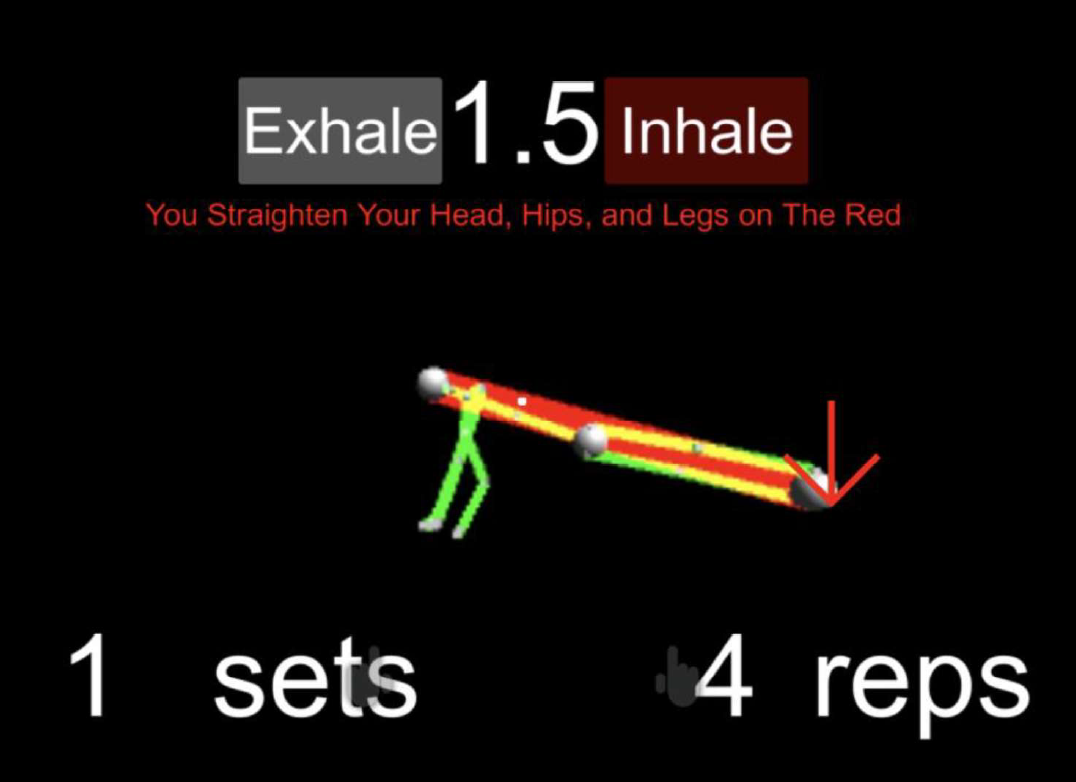
\includegraphics[width=\linewidth]{pictures/Oka.PNG}
    \caption{Color-coded skeleton: The skeleton visualizes where to correct the movement. Image from~\cite{oka2021rtf}.\label{fig:Oka}}
\end{figure}

Ikeda et al.~\cite{ikeda2018arb} likewise present a research attempt to visualize motion feedback using \emph{VR glasses}. Users can watch their body (as an avatar) from a \emph{third person} perspective. This enables them to gather information about the intended movement correction of the \emph{whole body}. It is possible to get the feedback in \emph{real time} as well as a \emph{playback} after the exercise. This work addresses the matching of actual and target movement with dynamic time warping. The matching of time discrepant executions is a challenge many real-time or playback feedback solutions have to face. The exocentric perspective in combination with VR is a setup often found throughout the literature surveyed. An example can be found in the work of Hoang et al.~\cite{hoang2016orp} and Ware et al.~\cite{ware2020wo2}.

Barioni et al.~\cite{barioni2019bvr} show \emph{upcoming} poses for the users to mimic. The target pose of the user is visualized by a \emph{transparent target avatar} which intersects an opaque avatar representing the user's actual pose (see \autoref{fig:Barioni}). The execution time of the pose is illustrated by a clock, which elapses when the pose is held correctly. The experimental setup uses a room-mounted \emph{display} as feedback technology, but the system can also be used with \emph{VR glasses}. The method of showing the poses before the execution is a typical way of providing information about the movement. It is often used in the literature at hand and can, for example, also be found in the work of Cao et al.~\cite{cao2020esa} and Han et al.~\cite{han2016ara}.
\begin{figure}[ht]
    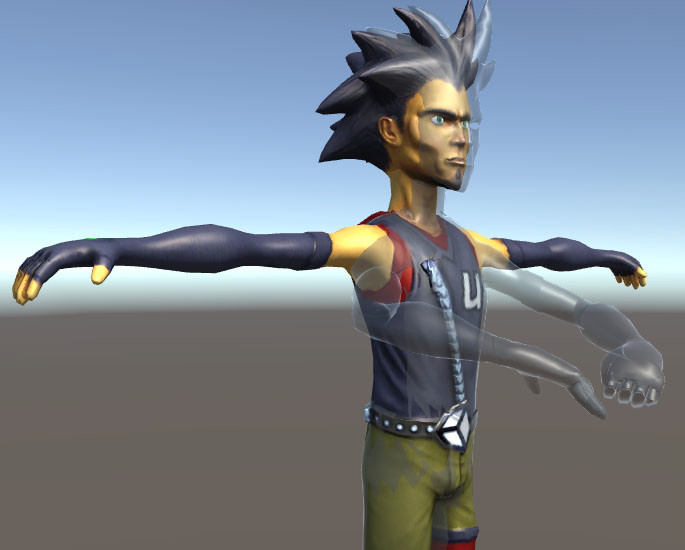
\includegraphics[width=\linewidth]{pictures/Barioni.png}
    \caption{An opaque avatar shows the actual pose, while a transparent target avatar depicts the target pose, which is to be taken. Image from~\cite{barioni2019bvr}.\label{fig:Barioni}}
\end{figure}

Oshita et al.~\cite{oshita2018sts} use \emph{opaque target avatars} to provide movement feedback for tennis shots. Additional \emph{arrows} show the \emph{direction} in which the correction is to be made and \emph{text} expresses how the movement should be executed. Furthermore, \emph{limb angles} are shown to depict the intended correction of a movement. After the execution, the feedback can be viewed on a large \emph{display}. The target avatar and avatars showing the actual user pose, together with the option of a \emph{playback} function is representative for many approaches in the surveyed literature. Examples of this combination can be found in the work of Hoang et al.~\cite{hoang2016orp} and Ikeda et al.~\cite{ikeda2018arb}. 

\subsection{Exceptional Examples}
A rehabilitation-oriented approach is presented by Debarba et al.~\cite{debarba2018arv}. With an \emph{optical see-through} HMD they visualize realistic-looking bones of the clients. The HMD is worn by the \emph{instructors}, who get \emph{real-time} feedback on how far the limb is bent by an angular indicator at the joint. The realistic rendering of bones is unique since it is often more legible to have abstract movement metaphors. Debarba et al. combine these realistic skeleton bones with a simple visualization of the \emph{limb angle}. This solution was chosen as an exceptional example due to the special circumstances of a rehabilitation setting in combination with the instructor as a feedback receiver.


The work of Shiro et al.~\cite{shiro2019ipv} represents another innovative attempt at giving feedback for movements. The system generates a picture with an interpolation between the pose of the user and a recorded movement of an expert. After the movement execution, the user can set how close the generated image should resemble the expert movement and browse through the timeline of the \emph{playback} as seen in \autoref{fig:Shiro}. This interpolation and image synthesis technique is quite exceptional in the surveyed literature. It utilizes generative adversarial networks (GAN), a machine learning (ML) technique, to synthesize the images and show a \emph{target pose} for the user to imitate.
\begin{figure}[ht]
    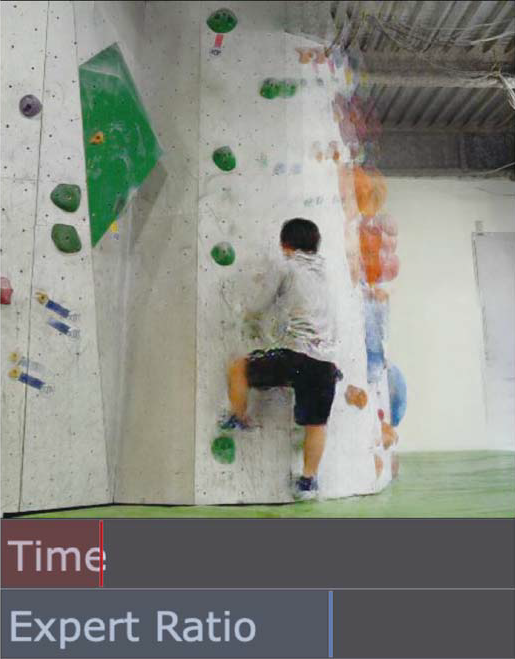
\includegraphics[width=\linewidth]{pictures/Shiro.png}
    \caption{Video frame synthesized by interpolating between user and expert pose. The upper slide bar represents the degree of expertise used for the interpolation. The lower slide bar controls the current frame of the playback. Image from~\cite{shiro2019ipv}.\label{fig:Shiro}}
\end{figure}

Vidal et al.~\cite{vidal2020blo} use a \emph{projection}-based approach to visualize the movement of the trunk. Lights attached to the body show the position of the trunk on the floor or walls of the room. The correct position is represented by a mark in the room. The users need to move to match this mark with the projected crosshair (see \autoref{fig:Vidal}). This \emph{abstract} approach, which works in \emph{real-time}, represents a singularity in the literature we analyzed.

\begin{figure}[bt]
    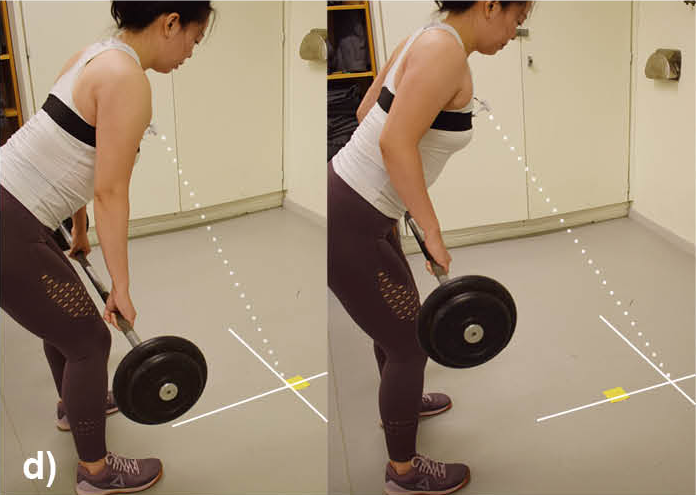
\includegraphics[width=\linewidth]{pictures/Vidal.png}
    \caption{Projection-based MR for body parts that are hard to see. Assuming a correct movement execution the projected crosshair matches the marking on the floor. Image from~\cite{vidal2020blo}.\label{fig:Vidal}}
\end{figure}

Another approach utilizing \emph{projection} is presented by Kosmalla et al.~\cite{kosmalla2017cvi}. A projector displays an image on a climbing wall visualizing either the \emph{end position} of the next motion or an instructor performing the \emph{upcoming} movement. The attempt to project the feedback onto the training equipment is seen a few times throughout the literature. It is the scale and the virtual instructor on the wall that make this approach unique.


\section{Survey Insights\label{sec:tvcg:insights}}
In this section, we will point out what we consider interesting findings of the classification seen in \autoref{table:2} and present what insights can be drawn from them. We discuss the insights by category.


\textbf{\emph{MR Technologies:}} The most used MR technology in the literature reviewed was \emph{room-mounted displays}, with \emph{VR-glasses} in second place. The reason for room-mounted displays and VR glasses as most used MR technologies could be accredited to the fact that they are simple and inexpensive to implement. Especially room-mounted displays used as "augmented mirrors" (see \autoref{sec:MR}), as often seen in the literature surveyed, can be set up with little inexpensive equipment like a camera and a normal display. Additionally, an augmented mirror approach provides an intuitive way to receive full-body feedback.

Contrary to our expectations, optical see-through headsets made up a small percentage of 15.4\% of the used technologies. Despite the important development the HoloLens represents, not many approaches utilize it to give visual motor feedback to participants in physical therapy and exercise.

\textbf{\emph{Point of View:}} More than half of the approaches used a third-person view in their systems. This can be directly linked to the high quantity of room-mounted displays as all of these systems use a third-person perspective.

\textbf{\emph{Abstraction Type:}} A majority of research attempts we surveyed featured a positional form of feedback. It is noticeable that most directional feedback is a hybrid of directional and positional feedback. Pure directional feedback could be hard for humans to comprehend. Only showing the direction is insufficient information in many cases, as it would be difficult for the participant to stop at the target location. Information about the distance is crucial to be able to move correctly and precisely without further compensating motions.

\textbf{\emph{Stages of Learning:}} Regarding the learning phases, the literature was predominantly categorized into the \emph{associative} phase. Although the stages are overlapping and therefore a clear assignment is sometimes impossible, the dominance of the approaches that can be classified as \emph{associative} can still be seen as significant. It could be argued that visual feedback is most appropriate in the associative skill learning phase. When subroutines are put together to form one uniform skill or movement the motor feedback might be most effective and useful to the user.

When considering the connection between the visual cues and the learning stages, we came to the conclusion that using graphs as visual cues might be most suitable for learners already familiar with the skill. Such learners would be in the \emph{autonomous} stage. New learners might be overwhelmed with the detailed information, and it might not contribute to their improvement. Advanced users, already in the autonomous stage, might look for ways to improve their movement beyond their self-reliant execution and can therefore be supported with graphs. Additionally, a \emph{guidance} feedback type could be helpful for learners in the cognitive phase since the upcoming movement is demonstrated, and they can take in the information about the movement.

\textbf{\emph{Publication Venue:}} When looking at the publication venues, we can see that a majority (82.1\%) of papers were published in a computer science venue. As expected most of the publications were found in the VR, AR, and MR sectors (35.9\%). Another substantial part (28.2\%) was found in the field of HCI. Furthermore, several (15.4\%) attempts were found in the fields of medicine, health, and sports. It is to mention here that research approaches in this sector often feature a different focus, for example, the medical state of the user or the impact of the system on performance. This sometimes culminates in the complete absence of statements or depictions regarding the visualizations employed in the publication. This led to an exclusion of such papers in the screening phase as described in \autoref{sec:tvcg:methodology}.

\textbf{\emph{Body Parts:}} Most feedback we observed was meant for the whole body. A few attempts concerned arms and legs and one paper covered feedback for hands. Again, it could be argued that this phenomenon is linked to the many examples of third-person augmented mirrors. Augmented mirrors are most suitable for a whole-body feedback type, as a mirror scenario is the most common way we experience the view of our whole body.

\textbf{\emph{Use Cases:}} The observation that many research attempts target individual sports seems trivial. HMDs for example are limited to one user. To give clear feedback only one user can be addressed. If a whole team of participants would have to get feedback it would be either very time-consuming or many systems would have to be available simultaneously. However, in team sports the feedback for specific movements is traditionally given to the individual.

\textbf{\emph{Visual Cues:}} The most popular visual cues were \emph{end position} and \emph{opaque target avatar} as seen in \autoref{fig:CueHistogram}. The directional cues like \emph{arrows} and \emph{rubber bands} are seldom used throughout literature. The literature appears to prefer a positional approach.

It becomes apparent that there are no clear outliers regarding the occurrences of visual cues. The literature does not seem to have found the best way to provide visual feedback in MR. This can be attributed to the wide variety of different use cases appearing in the literature surveyed and to the diversity of movements associated to these use cases.

\begin{figure}[tb]
    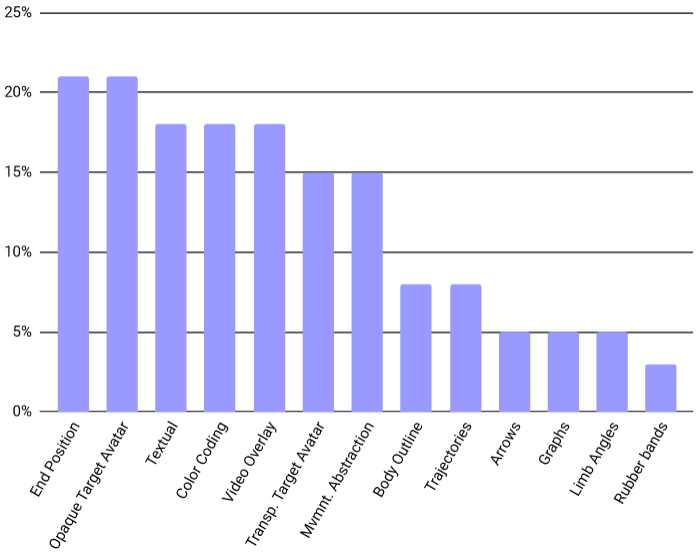
\includegraphics[width=\linewidth]{pictures/CueHistogram.PNG}
    \caption{Occurrence of different visual cues in the selected literature.\label{fig:CueHistogram}}
\end{figure}

\textbf{\emph{Evaluation Methods:}} Various different approaches to evaluating the methods and technologies can be found in the literature surveyed. Evaluations were mostly conducted from a \emph{therapeutic}, \emph{user experience} or \emph{visualization} standpoint and usually included a user study. The \emph{therapeutic} evaluations were mainly concerned with the recovery of the user or patient. For example, Booth et al.\cite{booth2019msr} measured the step length, knee extension, and ankle power of participants. Aside from their work \cite{booth2019msr}\cite{booth2019vue}, Afyouni et al.~\cite{afyouni2020arb}, Marti~\cite{marti2019evl}, Sekhavat et al.~\cite{sekhavat2018pba} and Karatsidis et al.~\cite{karatsidis2018vwv} provide therapeutic evaluations of their work as well.

A \emph{user experience} focused evaluation was found in the work of Cao et al.~\cite{cao2020esa}, Barioni et al.~\cite{barioni2019bvr}, Han et al.~\cite{han2016ara}, Hoang et al.~\cite{hoang2016orp} and Mostajeran et al.~\cite{mostajeran2019hvc}. These evaluations usually include a questionnaire to identify the condition or opinion of the participants. For example, Barioni et al.~\cite{barioni2019bvr} developed a questionnaire involving ten questions regarding the use of their system to obtain an opinion from the participants.

Evaluations from the visualization standpoint often include measures like precision or correction times. We observed this for example in the work of Yu et al.~\cite{yu2020pmd}, who measured completion time and movement error. Aside from that, similar metrics can be found in the approaches of Cao et al.~\cite{cao2020esa}, Kosmalla et al.~\cite{kosmalla2017cvi}, Barioni et al.~\cite{hoang2016orp}, Sekhavat et al.~\cite{sekhavat2018pba}, Sousa et al.~\cite{sousa2016sar}, Hülsmann et al.~\cite{huelsmann2019ssp}, Naour et al.~\cite{naour2019s3d}, Tang et al.~\cite{tang2015pah}, Trajkova et al.~\cite{trajkova2018ttb} and Waltemate et al.~\cite{waltemate2016tlp}.

Not always a clear distinction of these perspectives is possible. There are some works analyzing the feedback system from several standpoints for example Cao et al.~\cite{cao2020esa} and Hoang et al.~\cite{hoang2016orp}. Several more evaluations were found among the surveyed literature, but they either had a very small number of participants (\cite{oshita2018sts},\cite{meyer2018jlc}, \cite{escalona2020eva}, \cite{conner2016cef}) or did not deliver insights relevant for our overview (\cite{clarke2020rva}, \cite{han2016ara}, \cite{pereira2017jat}, \cite{caserman2021fbm}, \cite{vidal2020blo}, \cite{oka2021rtf}).

\section{Conclusion \label{sec:tvcg:conclusion}}
In this chapter, we gave an overview of the most recent literature on mixed reality feedback in the sector of physical exercise, rehabilitation, and general motor skill training. The literature has been classified and an overview of the classification is given in a table for easy reference. We discussed the different feedback types and identified potential for better utilization of feedback in the mentioned application areas.
We believe this survey closes a gap concerning a literature analysis by taking a closer look at visual cues. Furthermore, the survey could stimulate future research regarding visual cues for motor skill training as suggested in \autoref{sec:futureWork}.

\subsection{Findings}
We identified several trends:
\begin{itemize}
    \setlength{\itemsep}{-0.3cm}
    \item Many of the papers considered use approaches that can be described as virtual mirrors, that is a whole-body view on a display with feedback for certain movements.
    \item With respect to the abstraction type, positional feedback dominates the surveyed literature. Even directional feedback is often combined with the former to provide the user with sufficient information.
    \item In the examined approaches, feedback appeared to be mainly implemented for the associative skill learning phase.
    \item The papers used a variety of visual cues to pursue their goals. The most popular cues visualize the target pose or end position.
    \item The classification of literature in learning phases enables a more suitable feedback choice for specific target groups.
\end{itemize}

\subsection{Limitations}
This survey gives insight into which visual cues are utilized within the literature. We can only provide subtle hints to the reasons. An adequate analysis of the reasons for visual cue utilization is yet to be conducted. The chapter at hand does not deliver in-depth insights from a cognitive, therapeutic, or user experience standpoint.

As discussed in \autoref{sec:tvcg:methodology}, tool handling is not included in our scope. We solely focus on feedback for the human body. Nevertheless, several insights on visual cues and associated approaches might still be useful for supporting tool-based skill training with augmented reality.

There is no clear indication as to when Fitts and Posners~\cite{fitts1967HPe} learning phases apply, so the insights the classification can provide regarding this category are limited.

\subsection{Open Questions \label{sec:futureWork}}
At this state of research, the connection between feedback and learning stages~\cite{fitts1967HPe} is yet imprecise. It is still not always clear which visual cues are connected to which stages and what they invoke in users. It would be profitable to understand this connection better in order to improve motion learning in the sectors of rehabilitation, physical exercise, and private or professional skill training. With greater insight, the visual cues could be adjusted to better suit the target group and goal.

As mentioned in \autoref{sec:tvcg:insights} there are just a few research approaches with visual corrective feedback for team sports. It could be valuable to look deeper into the individual feedback given for team sports. Further, it might be interesting to study use cases where the interaction between the movements of two people is crucial, for example in dancing.

The insights found in this work could be transferred to tool handling. Since skill training is an important application for augmented reality, it might be interesting to analyze which of the visual cues found could be applied for tool-based skill training in the industrial context. This would build upon the work of Gatullo et al. \cite{gatullo2020whw}, applying it to the movement itself.

We found and discussed many different visual cues for motor feedback. Yet, the nature of them is not yet fully understood. It could be profitable to investigate the visual cues in more depth to allow for a better-informed choice. This chapter gives a first indication of when to use which type of feedback. Building upon the obtained insights, more detailed recommendations could be developed and researched in the future. To have a greater variety of visual feedback to choose from and intentionally utilize it for a given use case, one could investigate new visual cues especially tailored for mixed reality.


\externaldocument{content/viewpoint}
\chapter{Registration of Superimposed Avatars \label{chap:registration}}
\begin{figure}[ht]
	\centering
	\subfloat[Superimposition registered at pelvis]{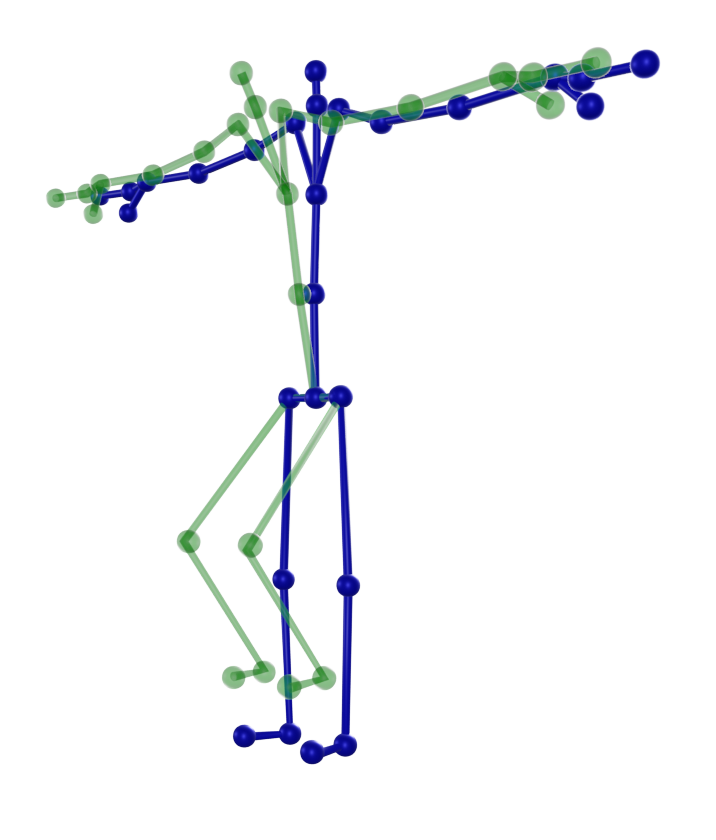
\includegraphics[height=0.35\linewidth]{pictures/pelvisReg.png}
		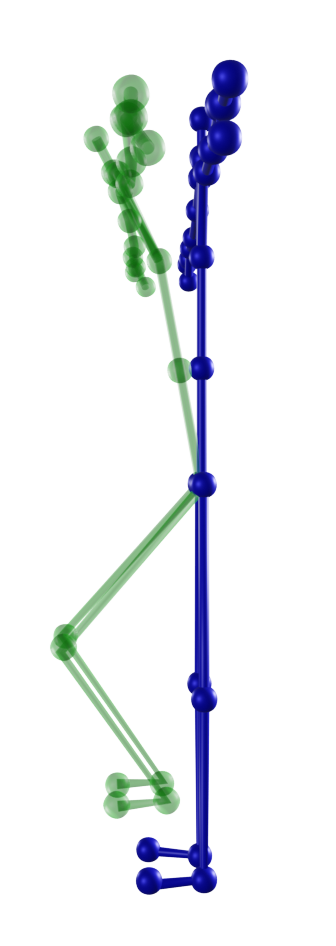
\includegraphics[height=0.35\linewidth]{pictures/pelvisRegSide.png}}
	\subfloat[Superimposition registered at feet]{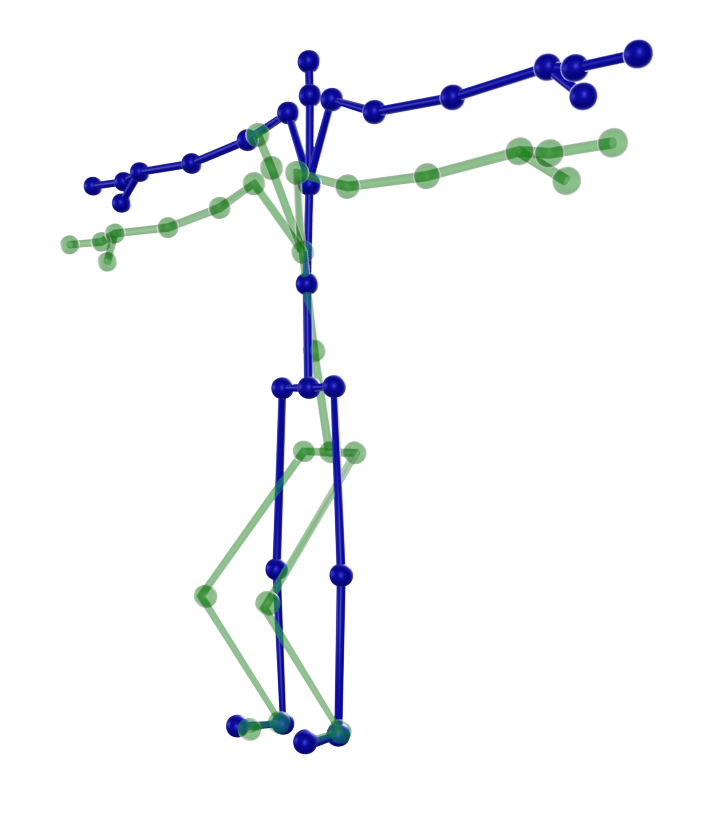
\includegraphics[height=0.35\linewidth]{pictures/footReg.png}
		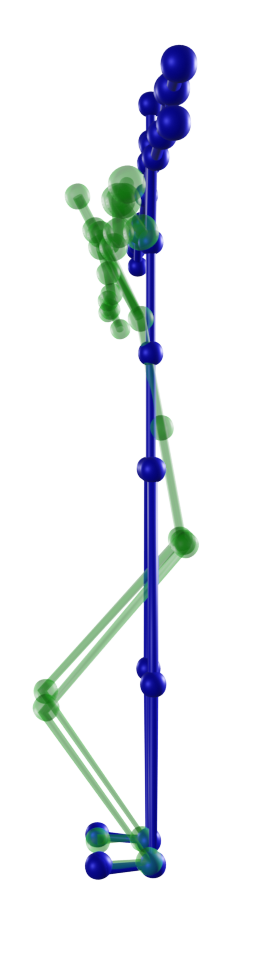
\includegraphics[height=0.35\linewidth]{pictures/footRegSide.png}}
	\caption[Illustrating the importance of registration.]{Illustrating the importance of registration: When registered at the pelvis (a), the squatting target avatar (in green) seems to be floating. Registering at the feet (b) seems to provide more intuitive feedback, connected to the environment.}
	\label{fig:registrationComparison}
\end{figure}

\section{Related Work \label{sec:relReg}}
In the current literature, we find a plethora of both rigid and non-rigid registration methods, as analyzed by Tam et al.~\cite{tam2012registration}. When registering an actual and target pose it is essential to use rigid registration, as we want to preserve potential deviations from the ideal form. These would be diminished by a non-rigid registration method, as it would deform the ideal avatar. Specifically for rigid registrations, there are several automatic methods, as Yaniv~\cite{yaniv2008rigid} and Bellekens et al.~\cite{bellekens2014survey} stated.

In some cases, a simple registration based on a single joint is completely sufficient. For example, to optimize posture guidance in \acrshort{vr}, Hoang et al.~\cite{hoang2016onebody} registered the target avatar based on the position and rotation of the pelvis. Instead, Anderson et al.~\cite{anderson2013youmove} used only the pelvis' position while maintaining the orientation of the recorded target movement. Subsequently, the approach was evaluated, and users performed two ballet and two abstract movements with the proposed system. In contrast, Naour et al.~\cite{naour2019superimpose} registered the avatars based on the position and rotation of the left foot. This way, the football-throwing motions of a learner were superimposed with those of an expert. Additionally, we find many approaches in the literature that register avatars but lack the explanation of methods.

\section{Methodology \label{sec:methReg}}
The registration of two exercises represents in most cases the foundation of visual feedback for motor skill training, in particular, superimposed avatars. When registering a superimposed actual and target avatar for a given exercise, we need to keep certain factors in mind to facilitate a better understanding of the scene for the user. For instance, the spatial relation of the avatars to the environment helps the user with orientation. Likewise, corrections for typical deviations have to be anticipated. In summary, a well-made registration can lead to a far more intuitive understanding of visual feedback.

The registration is directly linked to the other aspects of visual motor feedback in this work: For instance, it represents the foundation of how the visual cues analyzed in \autoref{chap:visualCueSurvey} are calculated.
Furthermore, the registration directly influences the inputs of the \acrfull{pca} viewpoint calculation in \autoref{chap:viewpoint} (i.e. $\Delta_n$ and  $\vec{v}_{Fn}$ in \autoref{eq:viewpoint} found in \autoref{sec:methViewCalc}). In addition, our \acrshort{pca}-based viewpoint method as explained in \autoref{sec:methViewCalc}, is designed to work with smaller deviations. Therefore, an appropriate registration method is important. Lastly, \autoref{chap:omnipresent} to great parts utilizes the avatar registration methods described in the following. Further detail is given there in \autoref{sec:register}.

\subsection*{Optimal Avatar Registration \label{sec:optimalReg}}
An optimal avatar registration is highly dependent on the specific exercise performed and even on the individual interpreting the visual feedback. However, there are a few key aspects that are crucial in helping users to comprehend feedback using superimposed avatars. In the following, we present guidelines, that can be used to register avatars for a certain scenario or to implement optimal avatar registration independently.

\begin{figure}[t]
	\centering
	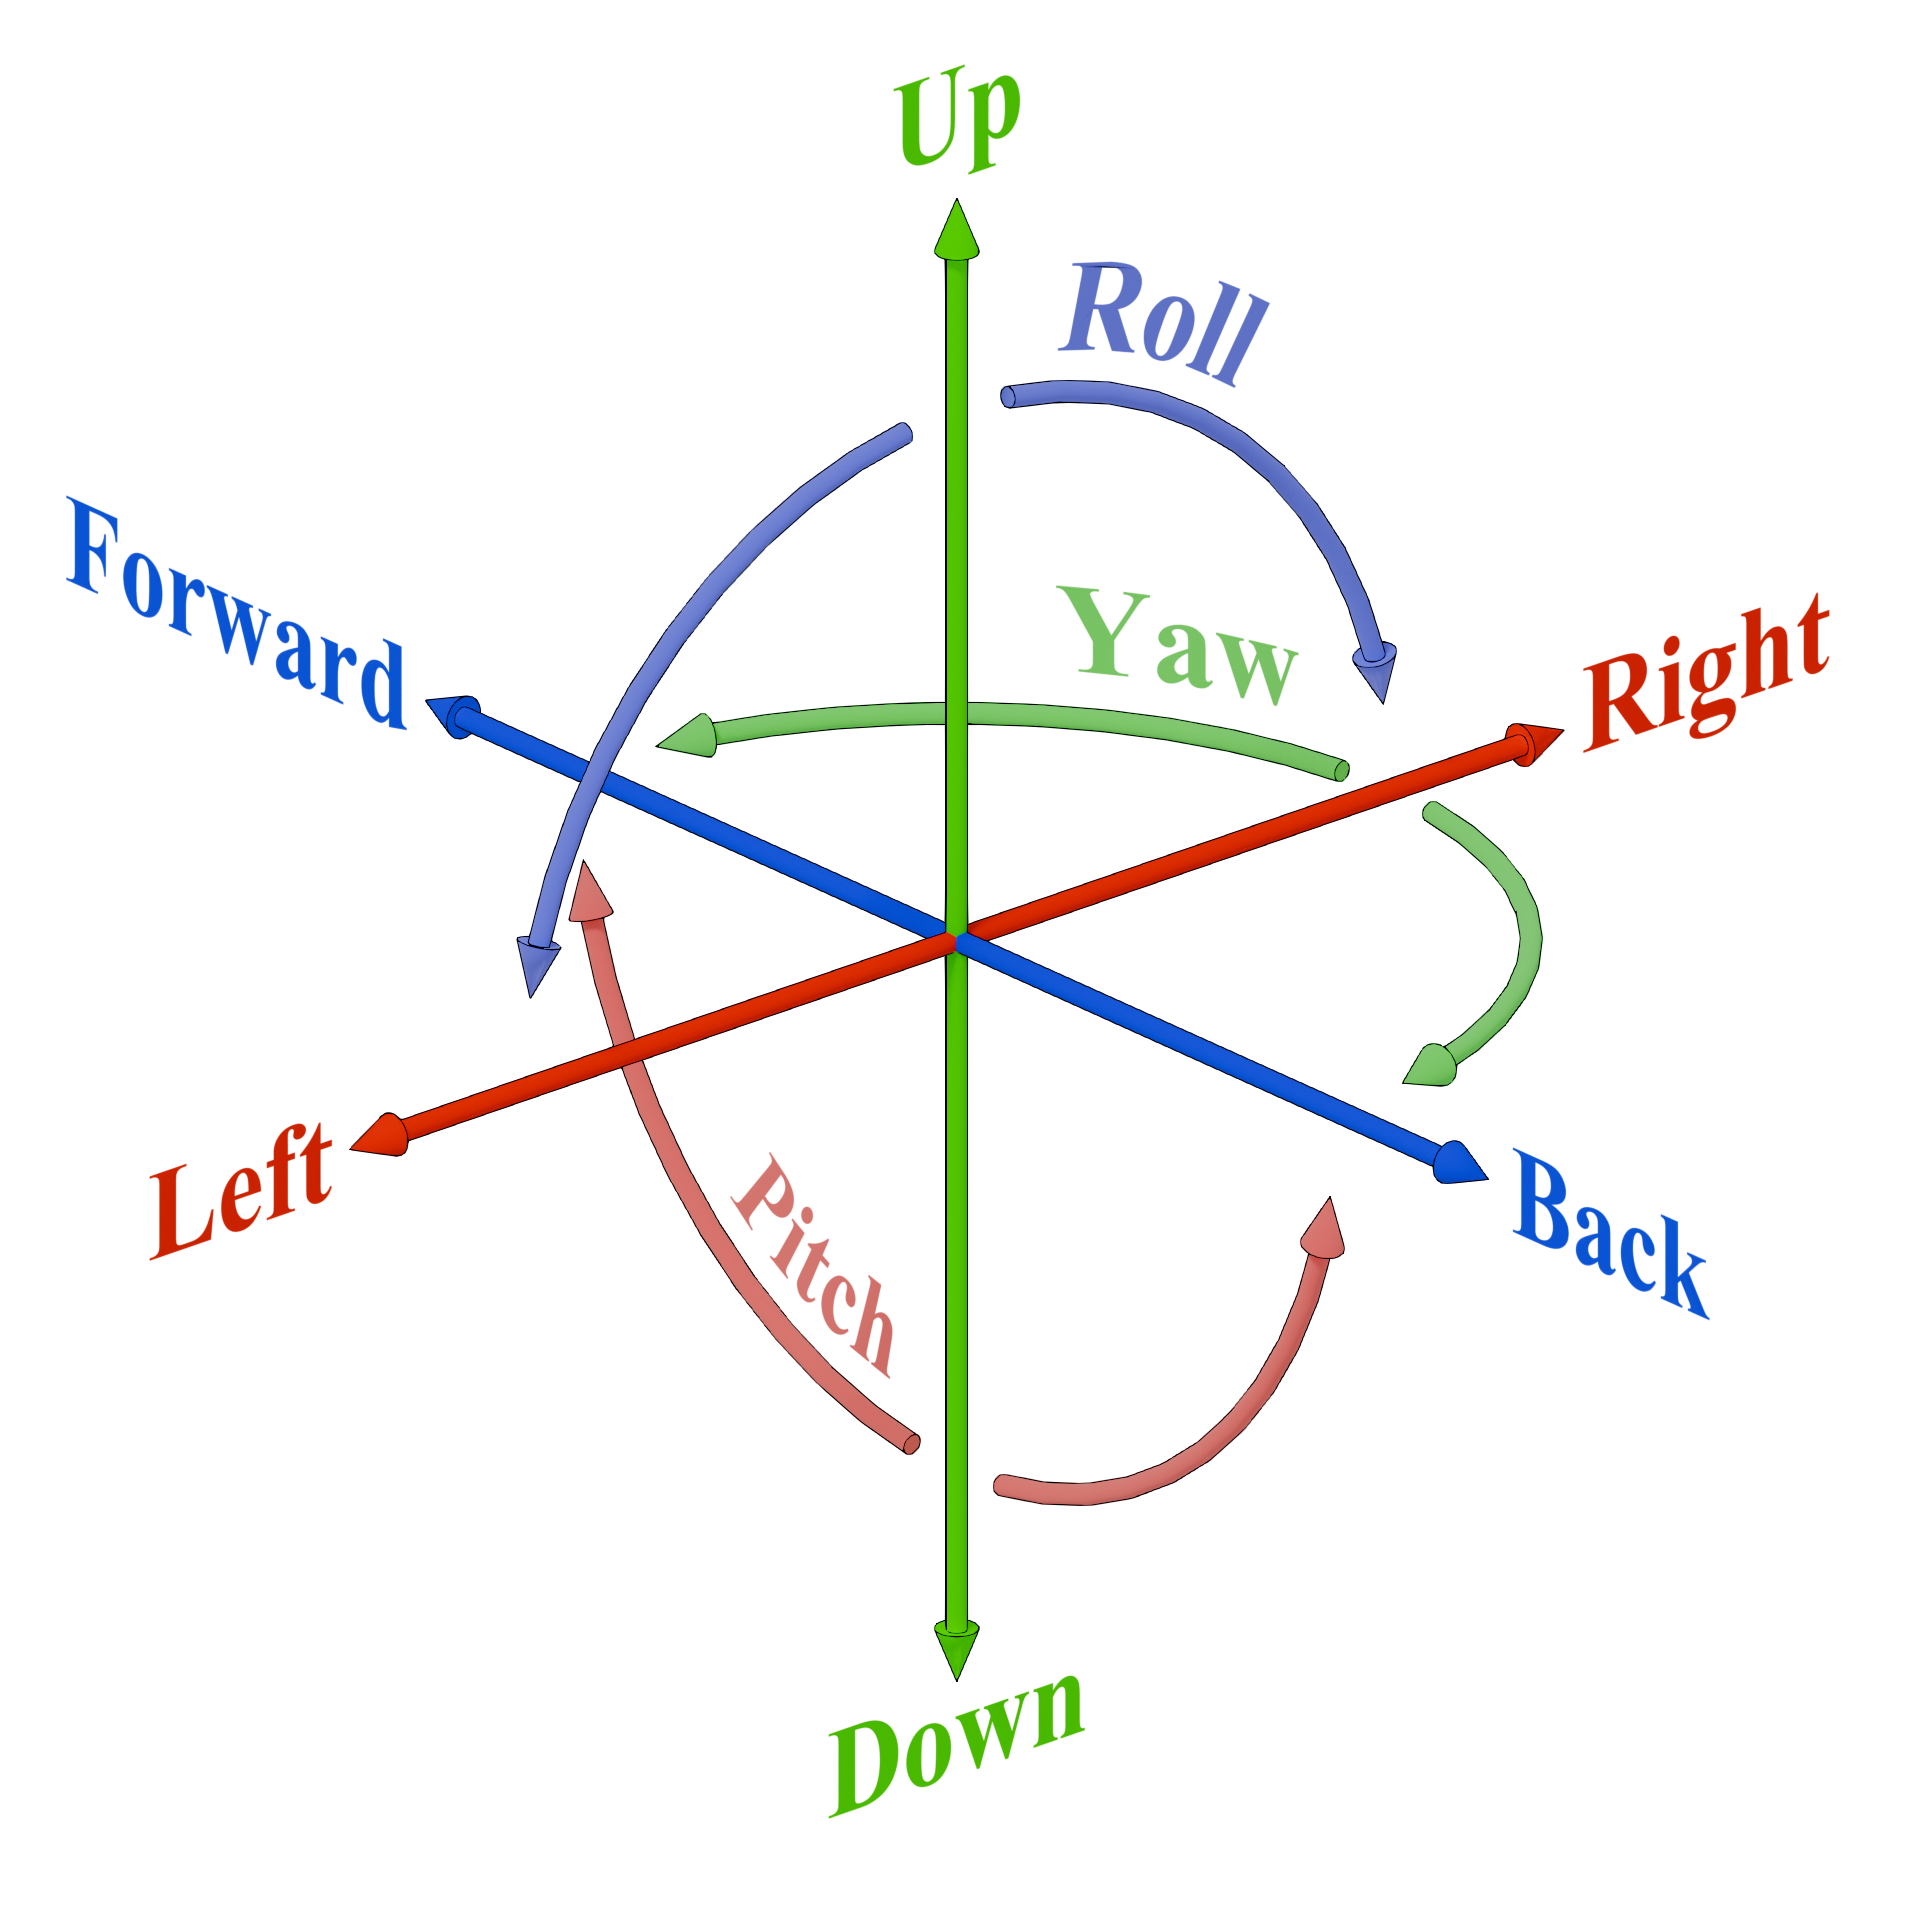
\includegraphics[width=0.5\linewidth]{pictures/Gizmos.png}
	\caption[\acrlong{6dof} to define the placement of a rigid body.]{\acrlong{6dof} to define the placement of a rigid body in space.}
	\label{fig:6dof}
\end{figure}

One single joint is oftentimes sufficient for registration. Especially for use cases with a limited selection of exercises, it can lead to satisfying results, as described in \autoref{sec:relReg}. However, to avoid irritating users, it is important to connect the avatars with their spatial surroundings. For this purpose, we consider the \acrfull{6dof} of a rigid body in 3D space, as depicted in \autoref{fig:6dof}. We combined the \acrshort{6dof} to form four different categories, adequate to optimize registration:
\begin{itemize}
	\setlength{\itemsep}{-0.3cm}
	\item Vertical alignment (up/down)
	\item Horizontal alignment (left/right \& forward/backward)
	\item Rotation about vertical axis (yaw)
	\item Rotation about horizontal axes (pitch \& roll)
\end{itemize}

To provide the best avatar registrations, we match these 4 different degrees of freedom with the following characteristics from the fixed avatar:

\textbf{Vertical alignment:} As mentioned above, it is crucial to connect the target avatar to the environment. Otherwise, the user might be irritated, as the avatars seem to defy the rules of physics. Depending on the exercise, there are different connections to the surroundings: When doing exercises while standing like squats or lateral raises, the feet rest safely on the ground, thus connecting the body with the environment. When hanging (e.g. pull-ups) or supporting the weight with the arms (e.g. dips) the hands connect the body to the outer world. Users expect the target avatar to be connected to the environment the same way. Consequently, the connection to the environment represents a good measure of aligning the avatars. That means when the user is standing on the ground, the avatar squatting seems to do the same (see \autoref{fig:registrationComparison}, b). We can further improve the registration if the lowest point is matched for horizontal alignment. This way, when the user lifts a foot, the avatar still stays on the ground. Especially concerning exercises on the ground, this step leads to a better understanding of what to do, even when standing in a neutral position.

\textbf{Horizontal alignment:} The torso represents a big and important part of the body and also contains the center of mass while standing. Therefore, a horizontal alignment of both the actual and target avatar proved to be most intuitive based on the torso. Slightly better results can be achieved when choosing the point closest to the limbs connecting to the environment (i.e. the pelvis for standing exercises, a point between the shoulders for hanging, etc.).

\textbf{Rotation around vertical axis:}
The rotation around the vertical axis plays an important part in registering two avatars. In most cases, this rotation represents the orientation within the environment, which is arbitrary except when working with stationary equipment. This means the rotation around the vertical axis can be freely adapted without compromising the correct execution of an exercise. As mentioned in \autoref{sec:relReg}, there are several joints with which the registration can seem intuitive, the joints in the torso emerge as the best option. In particular, using the same joint that we chose for the horizontal alignment delivers intuitive results when also used as a reference for vertical rotation.

\textbf{Rotation around horizontal axes:}
During exercise performance, the rotation around the horizontal axes (i.e. pitching and rolling) is highly dependent on the exercise. Altering these rotations can lead to false interpretations of the feedback. Therefore, we see these rotations as exercise-inherent measures, which should not be altered (or only with great care). Consequently, the pitching and rolling rotations might best be carried over from the exercise recording or reference movement. Otherwise, the avatars seem too adaptive, possibly leading to wrong movement execution.

\subsection*{Scaling}
When two avatars are superimposed, depending on the recorded individuals, the scale of the limbs is not necessarily the same. Scaling one avatar according to the total size of the other avatar only partially solves the problem. As the proportions (e.g. torso length compared to leg length) can differ between individuals, a uniform scaling can still result in inconsistencies. Therefore, if the recorded exercises compared potentially stem from different individuals, it is advisable to scale the target avatar bone-wise to match the actual live avatar. Here, it is important to ensure that the angles between the bones, i.e. at the joints,  stay consistent. Otherwise, the scaling will falsify the exercise. 

\subsection*{Registration Limitations}
Avatar registration is a complex subject. The most generally applicable guidelines can be found above. However, it seems as if there is no optimal approach for every individual, situation, and use case. Especially when considering the details concerning the rotation around the horizontal axes, it seems in some cases there is a trade-off between the exercise's validity and perfect registration.
Furthermore, scaling the target avatar eliminates most inconsistencies in a bone-wise fashion, yet the angles between the bones at the joints stay consistent. Consequently, given certain proportions and thus centers of mass of two individuals compared, the scaling could lead to the target exercise not being the most optimal. Although the methods mentioned above yield good results for most exercises, even when registering with a neutral standing position, hanging exercises are hard to perceive while standing. This results from missing reference points of the environment. Once the actual avatar is hanging, we can use the hands as reference points (in particular, horizontal alignment).

\begin{figure*}[tb]
	\centering
	\captionsetup[subfigure]{labelformat=empty}
	\subfloat[\centering Push-up (P)]{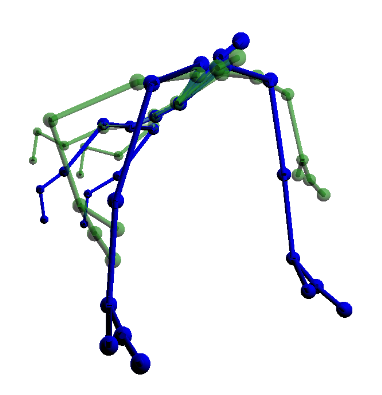
\includegraphics[height=.16\linewidth]{pictures/pushupPelvis.PNG}\hfill}  
	\subfloat[\centering Push-up (R)]{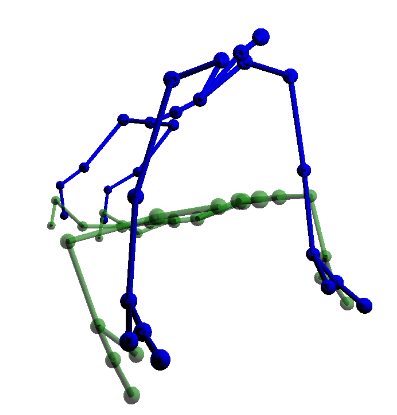
\includegraphics[height=.16\linewidth]{pictures/pushupRegistered.PNG}\hfill} 
	\subfloat[\centering Dip (P)]{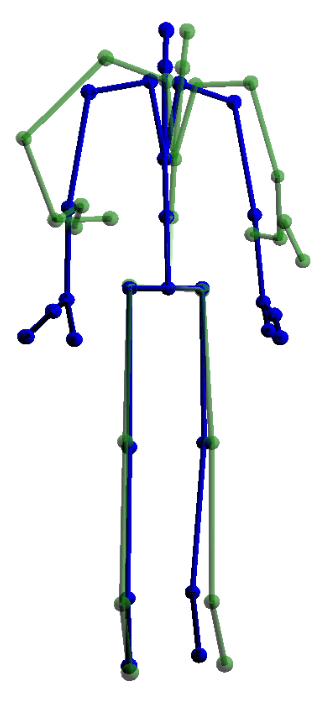
\includegraphics[height=.27\linewidth]{pictures/dipsPelvis.PNG}\hfill} 
	\subfloat[\centering Dip (R)]{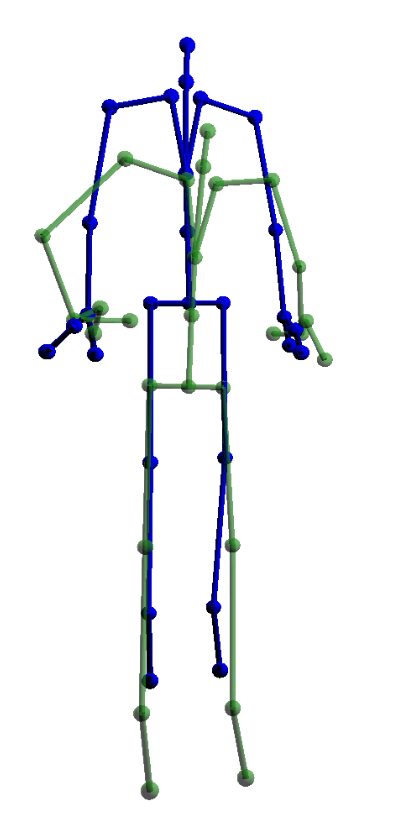
\includegraphics[height=.27\linewidth]{pictures/dipsRegistered.PNG}\hfill} 
	\subfloat[\centering Jump (F)]{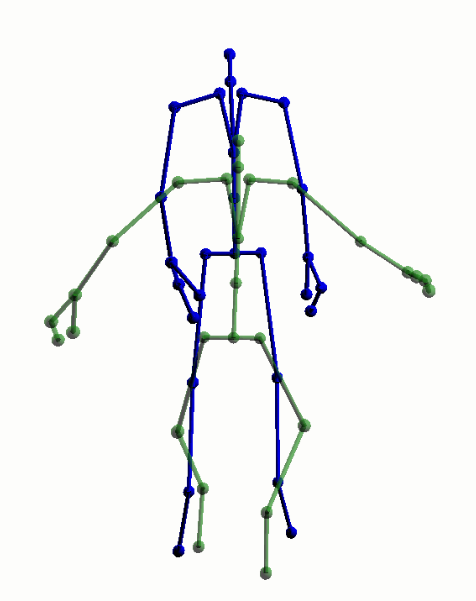
\includegraphics[height=.27\linewidth]{pictures/jumpFeet.PNG}\hfill}
	\subfloat[\centering Jump (R)]{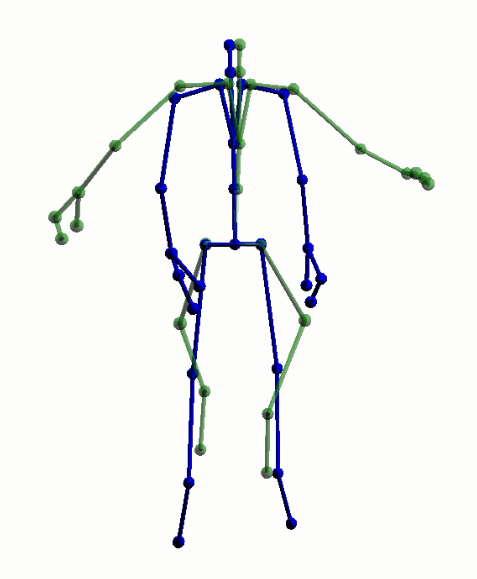
\includegraphics[height=.27\linewidth]{pictures/jumpPelvis.PNG}\hfill} 
	\caption[Registered start and execution position of exercise examples.]{Start and execution position of exercise examples registered according to our registration methods explained in \autoref{sec:optimalReg} (R), the feet (F) and only the pelvis (P). The exercises and registration parameters can be found in \autoref{tab:regExamples}.}
	\label{fig:regExamples}
\end{figure*}

\subsection*{Examples \label{sec:regExamples}}
To establish an understanding of the methods explained in \autoref{sec:optimalReg}, we chose a few exercises with corresponding joints to match the six degrees of freedom and will discuss them in this section. The exercises can be seen in \autoref{fig:regExamples} and the joints used for alignment can be taken from \autoref{tab:regExamples}. The examples were each chosen to be representative of a category of exercises. This selection is not intended to be complete, but rather a diverse collection, where finding examples close to many use cases is possible. Regarding registration, the example exercises could be sorted into 3 categories, as seen in \autoref{tab:regExamples}, based on how the individual connects with the environment:

\textbf{Connection to floor:}
Exercises that connect with the feet on the floor (like squats and warrior II), and those that involve lying down (like leg raises, plank, and push-ups) both profit from the same registration. Here, the pelvis was used to align the avatars on the horizontal plane. As a result, the torsos and therefore, the body's center were registered quite well. The avatars were vertically placed by aligning the lowest joint of each. Consequently, the avatars were intuitively placed on the floor, even if the movement of the actual avatar did not (yet) follow the target avatar (compare \autoref{fig:regExamples} and \autoref{fig:registrationComparison}). Concerning rotation, the pitch and roll rotations, as depicted in \autoref{fig:6dof}, were fixated similar to the recorded exercise. As already stated in \autoref{sec:optimalReg}, the pitch and roll rotations seem inherent to the exercise, as altering them can falsify the execution. However, the yaw rotation was based on the same joint used for horizontal alignment: The pelvis. This aligns the main orientations of the avatars.

\begin{table}[t!]
	\caption[Example exercises with corresponding registration.]{Exercise examples with corresponding joints for each of the six degrees of freedom to match for an optimized registration as described in \autoref{sec:optimalReg}.\label{tab:regExamples}}
	\footnotesize
	\begin{tabular*}{\textwidth}{@{\extracolsep\fill}lcccccc}
		\toprule%
		& \multicolumn{3}{@{}c@{}}{Translation along} & \multicolumn{3}{@{}c@{}}{Rotation around} \\\cmidrule{2-4}\cmidrule{5-7}
		& \multicolumn{1}{@{}c@{}}{Vertical axis} & \multicolumn{2}{@{}c@{}}{Horizontal axes} & \multicolumn{1}{@{}c@{}}{Vertical axis} & \multicolumn{2}{@{}c@{}}{Horizontal axes} \\\cmidrule{2-2}\cmidrule{3-4}\cmidrule{5-5}\cmidrule{6-7}
		Exercise & Up/Down & Left/Right & Forward/Back & Yaw & Pitch & Roll\\
		\midrule
		Squat  & Lowest Joint & Pelvis & Pelvis & Pelvis & Fixed & Fixed\\
		Leg raise  & Lowest Joint & Pelvis & Pelvis & Pelvis & Fixed & Fixed\\
		Push-ups  & Lowest Joint & Pelvis & Pelvis & Pelvis & Fixed & Fixed\\
		Warrior II  & Lowest Joint & Pelvis & Pelvis & Pelvis & Fixed & Fixed\\
		Plank & Lowest Joint & Pelvis & Pelvis & Pelvis & Fixed & Fixed\\
		Dips  & Hands & Neck & Neck & Neck & Fixed & Fixed\\
		Pull-up  & Hands & Neck & Neck & Neck & Fixed & Fixed\\
		Jump  & Pelvis & Pelvis & Pelvis & Pelvis & Fixed & Fixed\\
		\bottomrule
	\end{tabular*}
\end{table}

\textbf{Connection to equipment:}
Alternatively, during an exercise, the individual could connect with the environment on a piece of equipment. For example, this is the case when doing dips or pull-ups where the individual is either supported or suspended by the arms, as seen in \autoref{fig:regExamples}. As a joint for both, horizontal alignment as well as yaw alignment, the base of the neck (i.e. center between shoulders) was chosen. Here, this provides a more intuitive registration point than the pelvis, as the arms connect to the environment. For the same reason, the hands were chosen as the base for a vertical alignment. Since the bars for dips or pull-ups represent the connection to the environment, registration at the hands appears stable and intuitive.

\textbf{No connection to the environment:}
Lastly, some exercises require no connection to the environment (like jumping or swimming). Still, it is possible to register avatars in these cases. To do so, the pelvis is chosen as the center of the body, as seen in \autoref{fig:regExamples}. The pitch and roll rotations are again fixated on the target avatar from how the exercise was recorded. The remaining alignments (i.e. up/down, left/right, forward/backward, yaw) are all done according to the pelvis.

\section{Conclusion}
The consideration of avatar registration is inevitable when attempting to optimize the display of superimposed avatars. In the literature, avatars are often registered by aligning the position and/or rotation of a single joint. For specific use cases, this can be adequate. However, to ensure that users can easily understand a wide range of exercises, a more detailed approach must be taken. We offer valuable insights on how certain exercises could be optimally registered based on the performed exercise. Without the claim for completeness, we offer fundamental guidelines as the basis for application development or further research. Furthermore, we provide concrete examples to help with comprehension and potential implementation. Avatar registration, important by itself, additionally represents a major factor of influence on viewpoint selection, another essential topic for optimal display of superimposed avatars as illustrated in \autoref{chap:viewpoint}.
\externaldocument{content/registration}
\chapter{Automatic Viewpoint Selection for Interactive Motor Feedback Using Principle Component Analysis\label{chap:viewpoint}}
In modern society, skill training is crucial across various areas, including recreational sports, physical therapy, and professional environments. Enhancing the learning process through interactive technology is becoming increasingly important. Specifically, in motor skill training supported by mixed reality technologies, interactive visual corrective feedback has become particularly significant, as demonstrated in \autoref{chap:visualCueSurvey}. This feedback is designed to support individuals to perform specific body movements correctly, thereby reducing the need for constant supervision by professionals. Superimposed avatars, in various types, represent a particular prevalent feedback method. Proper execution of movements is vital in physiotherapy and physical exercise to achieve the desired benefits and prevent injuries. Additionally, the repetitive and controlled nature of movements in physiotherapy and strength training allows for precise feedback provision and the identification of common errors.

Despite their importance, current methods for viewpoint selection in human motion and action feedback do not adequately consider visual cues. Furthermore, many existing techniques are computationally intensive and unsuitable for real-time application. In contrast, this chapter identifies key factors for optimal viewpoint selection for superimposed avatars used for motor feedback and propose an algorithm for this purpose using \emph{principal component analysis} (PCA). This work explores valuable aspects of avatar registration. Not only do these directly impact the viewpoint selection, but they also give us a further understanding of how to register superimposed avatars to facilitate an understanding of the feedback from the user, independent of the rendering methods.

\section{Related Work \label{sec:relView}}
As demonstrated by Bouwmans et al.~\cite{bouwmans2018arpca}, robust PCA has numerous applications in the field of visual computing. For instance, Skaro et al.~\cite{skaro2021knac} introduced a method to reduce errors common in marker-based motion tracking.

Several studies have explored approaches to viewpoint selection for human actions or movements. For example, Rudoy et al.~\cite{rudoy2011vsh} developed a method to generate a three-dimensional volume from several successive frames to select the best physical camera for television broadcasts and similar applications. Whereas Kiciroglu et al.~\cite{kiciroglu2020amc} proposed an algorithm predicting pose estimation accuracy, facilitating drone navigation to the calculated view point. Shi et al.~\cite{shi2012ksb} introduced an algorithm to determine the best viewpoint using \emph{Kinematics Significance Based Saliency}, which orients figures and objects to show their most protuding features.

Wang et al.~\cite{wang2019asw} utilized information theory and deep reinforcement learning to select a single viewpoint for action sequences. In parallel, Choi et al.~\cite{choi2012rav} extracted key frames from motion data to create a sequence of stick figures representing the initial motion data.

\begin{figure}[ht]
	\centering
	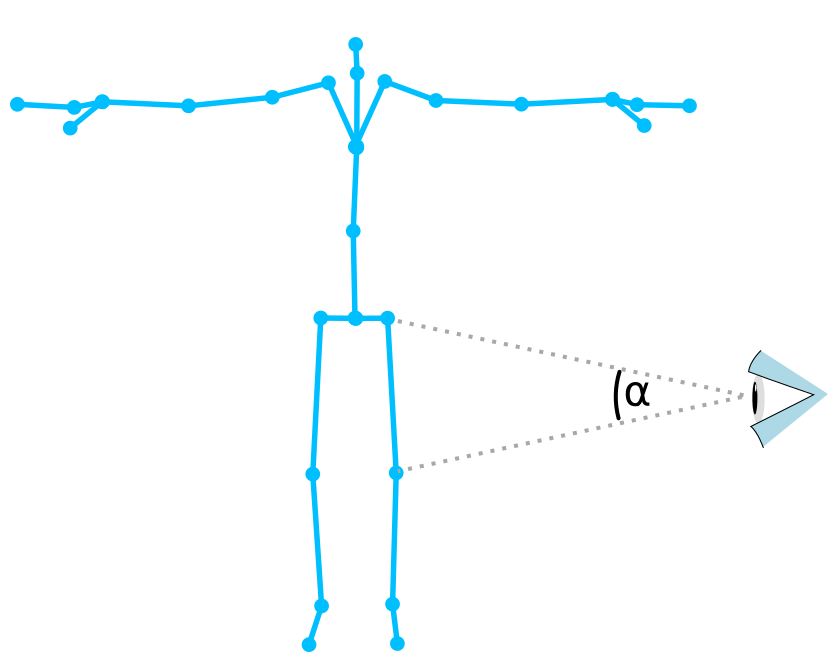
\includegraphics[width=0.6\linewidth]{pictures/skeleton_E_occ.png}
	\caption{Measure for the self-occlusion of the skeleton by Ishara et al.~\cite{ishara2015mra}: Joint Mutual Occlusion.}
	\label{fig:jmo}
\end{figure}

Ishara et al.~\cite{ishara2015mra} calculated the optimal camera position for robot navigation using a camera mounted on top of the robot. Their approach involves calculating the so-called \emph{Joint Mutual Occlusion} (JMO), which considers the angle \(\alpha\) between two joints and the viewpoint, as shown in \autoref{fig:jmo}. The angles \(\alpha_{nm}\) between joints \(n\) and \(m\) are summed and normalized, where \(n,m \in N\) and \(n \neq m\), with \(N\) representing the number of joints. This approach results in \(\frac{N!}{2(N-2)!}\) calculations of \(\alpha\)~\cite{charalambides2002enumerative} and could therefore be computationally expensive. 

Kwon et al.~\cite{kwon2020ocp} proposed a method that results in a weighted sum of three metrics: \emph{normalized limb length}, \emph{normalized area of a 2-D bounding box}, and \emph{normalized visible area of a 3-D bounding box}. In addition, they also presented an algorithm that avoids recalculating weights for each frame by summing the three metrics without weights. However, their algorithm, designed for static poses, requires recalculation for each frame in videos. Despite these methods automatically selecting camera positions for human poses, they are insufficient for visual feedback, as the skeleton can occlude the feedback, making it difficult to perceive, as analyzed by Nundy et al.~\cite{nundy2000wam} and discussed in \autoref{sec:considerations}.

The approaches by Ishara et al.~\cite{ishara2015mra} and Kwon et al.~\cite{kwon2020ocp} were compared to our method in a subsequent user study, as they were the only methods applicable to human figures with feedback. For more details, see \autoref{sec:evaluation}.

PCA is commonly used to reduce dimensionality in data sets for machine learning~\cite{sorzano2014sdr}. The principal components represent the main independent directions in which data points spread. For spatial data, three independent directions are involved. The first two principal components represent the main spread directions, while the third component provides a good viewing direction, perpendicular to the first two. This is equivalent to reducing the dimensionality from three to two, as the rendered image of 3D objects is displayed in two dimensions. Assa et al.~\cite{assa2008moh} used this method to calculate camera paths. However, their use case differs significantly, as they compute camera paths that involve camera cuts, which we avoid due to the short duration of exercise repetitions where cuts can be disorienting. Additionally, the work of Assa et al. is action-based, while ours is feedback-based, requiring additional measures to ensure feedback visibility. Lastly, their approach is not real-time capable, being computationally intensive and requiring the entire motion sequence for computation.

\section{Methodology \label{sec:view:methodology}}
\begin{figure*}[h!]
	\centering
	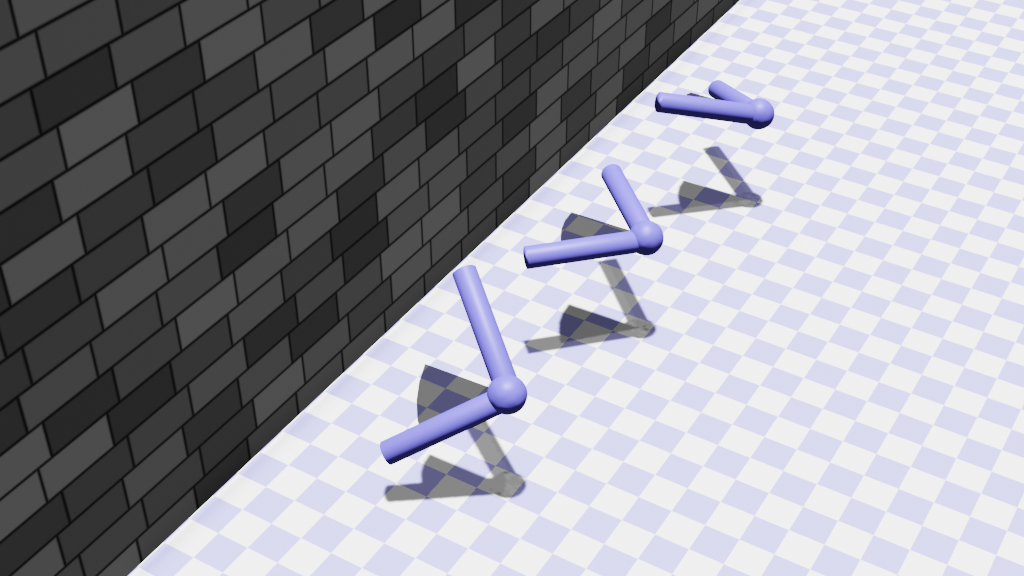
\includegraphics[width=0.49\linewidth]{pictures/projection_feedback}\hfill
	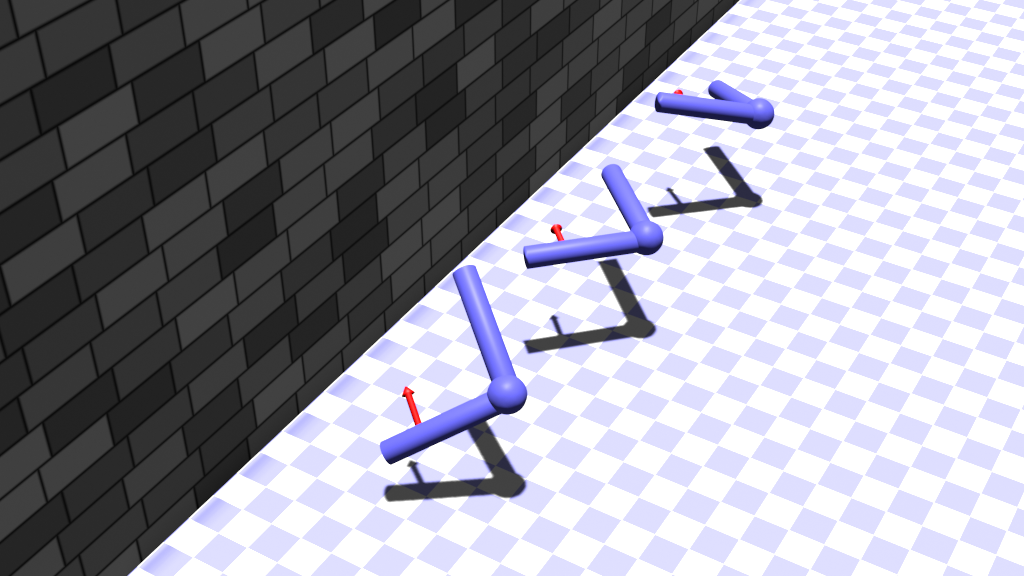
\includegraphics[width=0.49\linewidth]{pictures/projection_feedback_arrow}
	\caption{Feedback for the same angle viewed from different perspectives. Two feedback cues: circular sector (left) and arrow (right). From left to right: Perfectly visible, visible, and hardly visible feedback. The shadows demonstrate that viewpoint affects not only the perception of the geometry but also of the feedback.}
	\label{fig:projection_feedback}
\end{figure*}
To facilitate a user-friendly and intuitive viewpoint selection, several things have to be considered. We will discuss these in detail in \autoref{sec:considerations}. With the foundational registration methods discussed in \autoref{sec:optimalReg}, it is possible to calculate an optimized viewpoint, as presented in \autoref{sec:methViewCalc}.

\subsection*{Perspective Considerations \label{sec:considerations}}
In the literature, concrete rules for generating good perspectives are lacking. However, based on user preferences and logical argumentation several criteria and hints can be extracted to determine what facilitates a good viewpoint.

\begin{figure}[t!h]
	\centering
	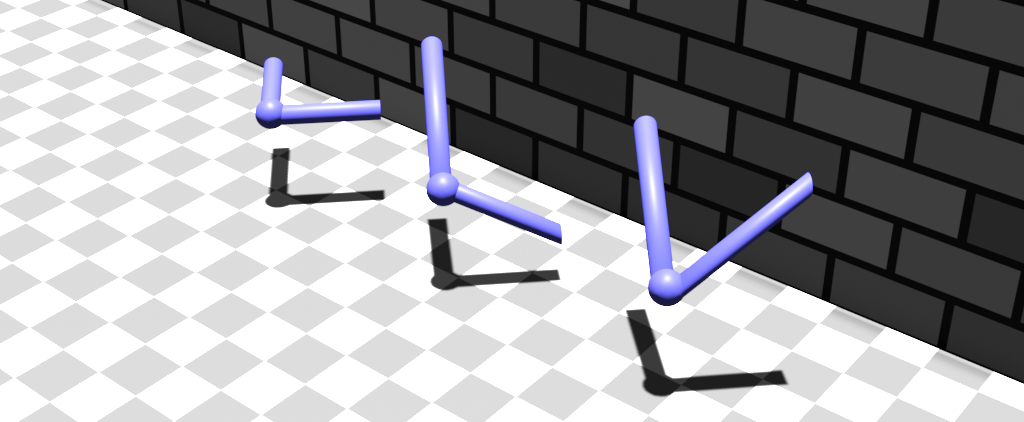
\includegraphics[width=\linewidth]{pictures/projection_normal.png}
	\caption{Highlighting the importance of viewpoint selection: Three \emph{different} joint angles produce \emph{identical} shadows when projected onto the ground, implying they appear identical from an overhead perspective. Inspired by Nundy et al.~\cite{nundy2000wam}.}
	\label{fig:projection_normal}
\end{figure}

Polonsky et al.~\cite{polonsky2005wii} identified seven measurable view descriptors but concluded that determining a universally good view of an object is challenging. None of the view descriptors alone provides a general measure of viewpoint quality. However, some clues are available for treating specific objects. For instance, Zusne~\cite{zusne1970vpf} empirically demonstrated that humans prefer a frontal view of objects with eyes and a face.

When looking at motor feedback, here in particular superimposed avatars, the positions of the joints and the angles between limbs are particularly critical for understanding movements. However, as previously analyzed by Nundy et al.~\cite{nundy2000wam}, angle perception is highly perspective-dependent. This is especially true in computer-rendered perspectives due to screen projection distortions, as shown in \autoref{fig:projection_normal} and \autoref{fig:projection_feedback}. While stereoscopic viewing (e.g., in the real-world or via HMD) helps depth perception and angle interpretation, monoscopic rendering does not offer the same possibilities. Additionally, occlusion can impede understanding of the human pose, with self-occlusion of the avatar's limbs behind each other. Similarly, visual feedback cues can be obscured by the avatar itself or by other cues, as depicted in \autoref{fig:projection_feedback} and \autoref{fig:skeletonFeedbackPerspective}.


\begin{figure}[t!h]
	\centering
	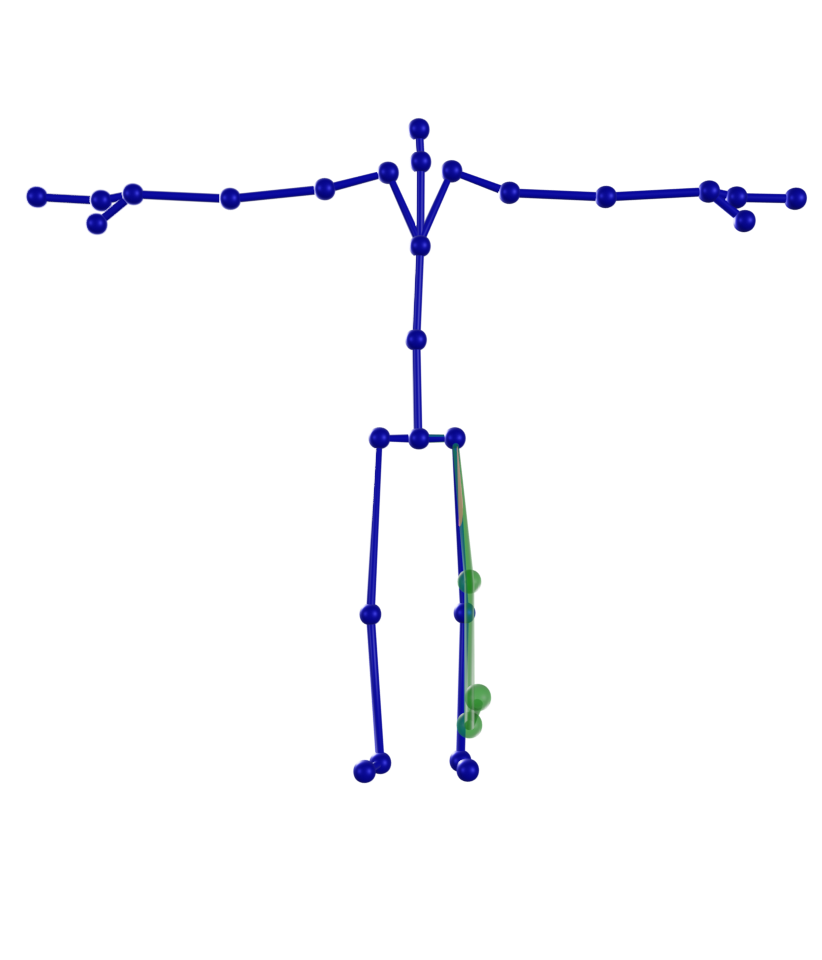
\includegraphics[width=0.49\linewidth]{pictures/feedbackFront.png}
	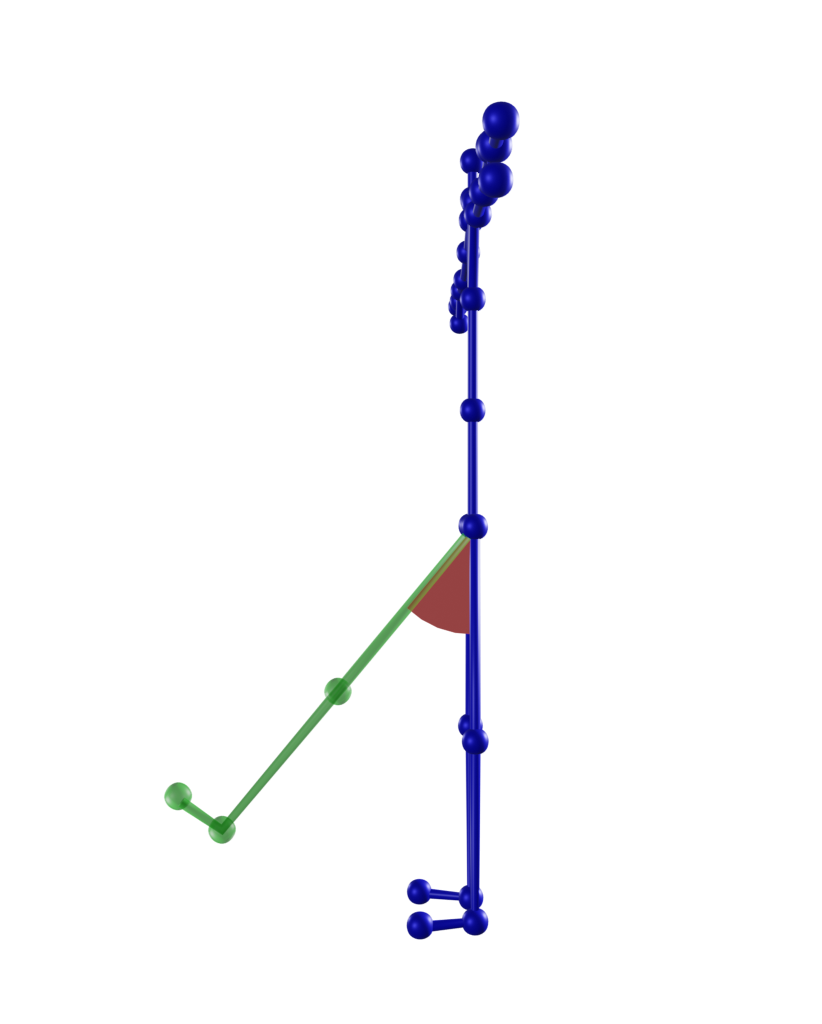
\includegraphics[width=0.49\linewidth]{pictures/feedbackSide.png}
	\caption{Skeleton of a human pose with feedback from two perspectives. Two visual feedback cues are shown: A red angle sector and a superimposed avatar (here green skeleton). The feedback is hardly visible from the frontal perspective on the left.}
	\label{fig:skeletonFeedbackPerspective}
\end{figure}

Given the lack of a general description for a good view, we need to define the characteristics of a good viewpoint for our specific use case. In our context, we frequently use the metaphor of a virtual camera, common in rendering, to describe the viewpoint and viewing direction. Following Zusne's~\cite{zusne1970vpf} findings, we prefer an approximately frontal view of the human pose, meaning the virtual camera should be oriented towards the front of the pose rather than from behind. Additionally, the camera's up-vector should align with the world's up-vector to avoid viewer confusion, as this is the biologically typical perception for humans. Furthermore, we aim to minimize the occlusions of the avatars demonstrating the movement execution. Finally, in our use case, visual feedback is provided to correct movements or poses, and this feedback must be clearly visible. Therefore, feedback should not be occluded by the avatar or by itself and should be as perpendicular to the view direction as possible.

When selecting perspectives for human motions and corresponding feedback, it is important to consider the dependencies of different body parts. Specifically, the limbs are hierarchically linked, meaning that moving the upper arm will cause the lower arm and hand to follow. Consequently, perspectives for such motions should ideally employ a \emph{hierarchical drill-down mechanism} to prioritize viewing along the hierarchy.

\subsection*{Viewpoint Calculation \label{sec:methViewCalc}}

As presented in \autoref{sec:relView}, the existing literature does not yet provide an optimal viewpoint calculation for human motions with visual feedback suitable for skill learning. Most approaches are optimized for human actions, leading to the potential invisibility of feedback from an action-optimized viewpoint. In the following, we guide you through our computationally inexpensive method for calculating a viewpoint for human actions with feedback. \autoref{eq:viewpoint} shows the calculation of our view direction $\vec{v}_d$:

\begin{equation}
	\label{eq:viewpoint}
	\vec{v}_d = w \cdot \vec{v}_{S} + \sum_{n=1}^N (\Delta_n - \delta_0) \cdot \vec{v}_{Fn}
\end{equation}

Calculating $\vec{v}_d$ involves the following variables: \(w\) represents a weight to adjust the impact of the view between the whole skeleton and the feedback; \(\vec{v}_S\) is the viewpoint optimized for all joint coordinates (i.e., the actual skeleton); \(N\) represents the number of joints that exceed a given deviation threshold \(\delta_0\); \(\Delta_n\) is the deviation of a joint \(J_n\) from the intended target position; the variable \(\delta_0\) is a constant threshold of the deviation; and \(\vec{v}_{Fn}\) is the view direction optimized for the feedback corresponding to joint \(J_n\), i.e. the deviating of \(J_n\) and its corresponding joints, as seen in \autoref{fig:eigenvector}. We do not consider rotations in the calculation, because they also inevitably cause deviations in distance.

Some motion capture systems provide recorded spatial data as three-dimensional joint coordinates (see \autoref{sec:recording} for our data acquisition method). When we conduct PCA over such a point cloud of joint coordinates, the first two eigenvectors \(\vec{e}_{1S}\) and \(\vec{e}_{2S}\) represent the two main spatial spread directions. The third eigenvector \(\vec{e}_{3S} = \vec{v}_S\), perpendicular to the first two, consequently providing a well-suited view direction $\vec{v}$ for all joints, as explained in \autoref{sec:relReg}. In other words, the point cloud representing the whole skeleton is most spread out along the horizontal and vertical axes of the captured camera picture. Consequently, the view direction \(\vec{v}_S\) is optimal for comprehending motions and poses. This method is also presented in Assa et al.~\cite{assa2008moh}.

Because the view direction should be optimized for corrective feedback corresponding to the deviations of the exercises, we must consider the deviating joints. For this purpose, we locally apply the above-mentioned PCA viewpoint calculation. The PCA is conducted with the actual and target joint coordinates and the corresponding parent joint coordinates as seen in \autoref{fig:eigenvector} for joints \(J_n, n \in [1..N]\), with deviations \(\Delta_n\), that exceed the deviation threshold \(\delta_0\). Consequently, the resulting eigenvector \(\vec{e}_{3Fn} = \vec{v}_{Fn}\) is a suitable view direction for displaying joint \(J_n\), its parent, the corresponding optimal joint position, and its parent. This is illustrated in \autoref{fig:eigenvector}, where the considered joint \(J_n\) is shown in red, the optimal joint position in orange, and the corresponding parent joints are depicted in blue.

\begin{figure}[tb]
	\centering
	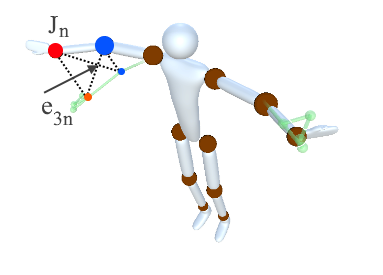
\includegraphics[width=0.5\linewidth]{pictures/eigenvector.png}
	\caption{If Joint \(J_n\) (in red) deviates from the target position, a PCA is conducted including the corresponding target joint (in orange) and their parents (in blue). The eigenvector \(\vec{e}_{3n}\) then gives us an optimal view direction \(\vec{v}_{Fn}\) of the feedback for \(J_n\). The resulting view direction is orthogonal to the plane defined by the eigenvectors \(\vec{e}_{1n}\) and \(\vec{e}_{2n}\). This plane approximates the distribution of the considered joints and does not interpolate them.}
	\label{fig:eigenvector}
\end{figure}

In \autoref{eq:viewpoint}, the factor \(\Delta_n\) (minus the threshold \(\delta_0\)) of \(\vec{v}_{Fn}\) increases the influence of joints depending on their deviation. This automatically considers a hierarchical drill-down mechanism (see \autoref{sec:considerations}), since lower hierarchy joints (farther from the body center) usually have a higher absolute deviation, as they are impacted by the deviations of the higher hierarchy joints (closer to the body center), adhering to the intercept theorem. The subtraction of the threshold \(\delta_0\) ensures continuous camera movement, so that the impact of deviating joints continuously increases or sets in from zero. The sum of all \(\vec{v}_{Fn}\) represents a feedback-optimized view direction for all joints exceeding the deviation threshold. This could be seen as the calculation of the mean of all \(\vec{v}_{Fn}\) without the division. The division is unnecessary, as the length of the view direction vector is irrelevant.

The view direction optimized for the skeleton \(\vec{v}_S\) is weighted with the constant \(w\) to adjust optimization between the skeleton and feedback. Values of \(\delta_0 = 50\) and \(w = 3\delta_0 = 150\) showed the best empirical outcomes for our use case. This holds several implications:
\begin{itemize}
	\setlength{\itemsep}{-0.3cm}
	\item The eigenvectors resulting from the PCA, and therefore the view direction vectors, are normalized, i.e. they have a length of 1. In the virtual 3D space, we applied a scale of \(1\ unit = 1\ mm\). Consequently, the deviation threshold \(\delta_0\) corresponds to \(50\ mm\).
	\item To have the same impact as the skeleton-optimized view direction \(\vec{v}_S\), the feedback-optimized view direction \(\vec{v}_{Fn}\) of a single joint would need to have a deviation of 200 mm, consisting of a 50 mm minimal threshold plus 150 mm of weight.
	\item The deviations of several joints together can exceed 150 mm (plus threshold) to have the same impact on the resulting view direction as the skeleton as a whole.
	\item If multiple joints do not exceed the 50 mm minimal threshold, the skeleton has 100\% impact, thus the viewpoint is optimized for just the skeleton.
	\item Because we consider the absolute deviation (instead of relative to the parent), the deviations of lower hierarchy joints and their parent joints are dependent. This results in a hierarchical drill-down mechanism, as explained in \autoref{sec:considerations}, where the joints closer to the body center have a higher impact on the view direction.
\end{itemize}

To calculate the viewpoint for the virtual camera, we subtract the normalized view direction \(\vec{v}_d\) from the location of the focus point, which will be centered in the rendered frame (in our case, the joint representing the pelvis location, since it is a good representation of the body's center). The distance to the focused point can be set by multiplying a constant. The digital distance corresponding to 2 m yielded the best results for us, as all exercises were in frame at this distance. However, this highly depends on the settings (e.g., focal length) of the virtual camera chosen.


If \(\vec{e}\) is an eigenvector, \(c \cdot \vec{e}\) is also an eigenvector, for all \(c \neq 0\)~\cite{borisenko}. Consequently, \(-\vec{v}_d\), the flipped eigenvector of \(\vec{v}_d\), is also a viable view direction. Initially, we select the direction resulting in a more frontal view of the avatar, since this is the predominantly preferred view~\cite{zusne1970vpf}. For every subsequent frame, we select the direction (from 
\(\vec{v}_d\) and \(-\vec{v}_d\)) with a smaller angular difference from the previous frame's direction, ensuring smooth camera motion.

Although the third eigenvector of the PCA follows a smooth path, the view direction (i.e. camera) tends to rotate around the avatar, contradicting Zusne's~\cite{zusne1970vpf} findings that a frontal view is commendable. To resolve this, we projected view angles from behind to the frontal plane, bypassing the predominantly small number of frames that feature a view from behind and showing a view from the side. Consequently, the projection affects the camera view only slightly and briefly.

Existing view selection approaches often focus on solving an optimization problem, iterating over a limited number of potential viewpoints, and choosing the one with the best score. This can result in a high number of costly iterations or erratic camera motion if the number of potential viewpoints is too small. Additionally, the best-scoring viewpoints in consecutive frames might be far from each other, resulting in inconsistent camera movements. Our method, however, provides continuous camera movement, as none of the mathematical operations in \autoref{eq:viewpoint} compromise consistency, and the PCA computations are conducted for continuously moving point clouds.

Empirically, no cases were encountered where a null vector arose from the calculations above. We also assessed stability regarding the PCA, as it is mathematically possible, that the camera view flips if the second and third eigenvectors have approximately the same length and deviate just slightly. In our experiments, this never occurred.

\section{Viewpoint Selection Evaluation \label{sec:evaluation}}
To verify the viewpoint selection method described in \autoref{sec:methViewCalc}, a user study was conducted. The necessary preliminaries, the study design, and the subsequent evaluation methods are found in the following.

\subsection{Participants}
For the user study, 39 individuals were recruited from an academic environment. These were predominantly computer science students between the ages of 20 and 30. More than half of the participants reported frequently exercising and considering movement-related aspects, giving ratings of four or higher on a five-point scale. This shows that the participants were somewhat acquainted with similar exercises and their execution. By comparison, much less physiotherapy clients were represented in the study. More than half of the participants reported receiving physiotherapy with the lowest frequency. Color vision deficiency did not affect our user study because the tasks required participants to recognize shapes rather than colors, as our focus was on perspective.

\subsection{Experimental Setup for Exercise Recording\label{sec:recording}}
The poses and motions found in this work were recorded using a Microsoft Azure Kinect 3D camera~\cite{kinect:documentation}. Its computer vision capabilities can provide spatial coordinates of several joints of the human body. Here, the term \emph{joint} is rather defined as biological landmarks than referring to the medical definition~\cite{kinect:documentation}.

The following conditions achieved optimal positioning of the subject in our case: The camera was mounted at about 140~cm with the help of a tripod. It was placed about 280~cm away from the subject. The height of the subject was about 190~cm. This setup allowed for stable tracking and captured all poses within the frame. According to our use case, the joints of the eyes, ears, and nose were discarded as we found that these were too imprecise and irrelevant to our use case. This left us with 26 joints. For further information on the visualization of avatars, see \autoref{sec:exercise}.

Subsequently, a diverse set of example exercises was developed including various exercise and deviation combinations. We then superimposed each of these exercises to the corresponding counterpart with deviation from the correct form (see \autoref{sec:sample}). The spatial registration was unambiguous, as the majority of joints were nearly identical. For further information regarding registration, covering more complex cases, see \autoref{sec:methReg}. The methods used to create an overlay of two exercises matching temporally exceed the scope of this chapter. Throughout the literature we often see \emph{Dynamic Time Warping} fulfilling that role (e.g., \cite{su2013pre}, \cite{anton2015pre}, and \cite{saenz2016kbv}).


\begin{figure*}[t!]
	\centering
	\subfloat[\centering Bench press]{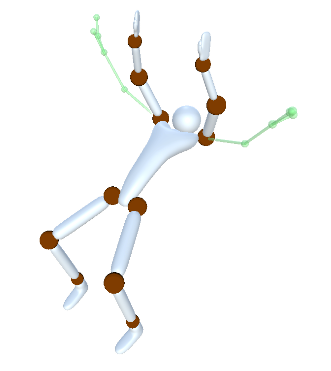
\includegraphics[width=.18\linewidth]{pictures/bench.png}\hfill}  
	\subfloat[\centering Curl A]{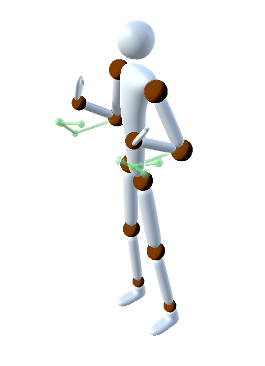
\includegraphics[width=.14\linewidth]{pictures/curlA.png}\hfill} 
	\subfloat[\centering Lateral raises]{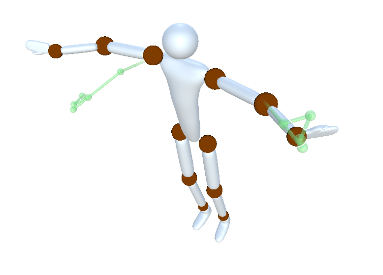
\includegraphics[width=.18\linewidth]{pictures/lateral.png}\hfill} 
	\subfloat[\centering Shoulder press]{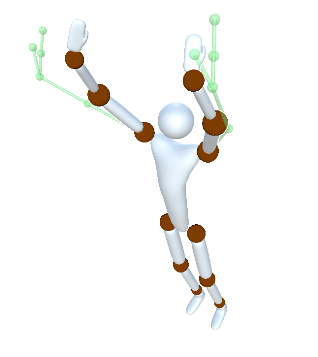
\includegraphics[width=.18\linewidth]{pictures/shoulder.png}\hfill} 
	\subfloat[\centering Bent-over\\row]{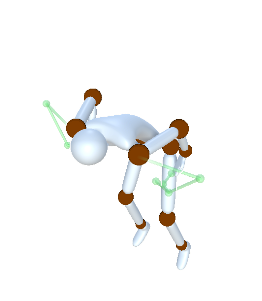
\includegraphics[width=.18\linewidth]{pictures/rows.png}\hfill}
	\subfloat[\centering Curl B]{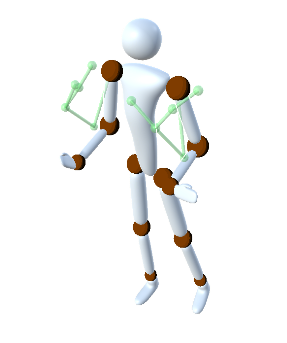
\includegraphics[width=.14\linewidth]{pictures/curlB.png}\hfill} 
	\caption{Sample exercises with deviations as described in \autoref{sec:sample}.}
	\label{fig:optimal:exercises}
\end{figure*}

\subsection{Exercise Visualization \label{sec:exercise}}
An abstract avatar was used to visualize the actual motion, and for the target motion, a skeleton is displayed as seen in \autoref{fig:optimal:exercises}. The visualization of the skeleton displayed in green corresponds to the joints recorded by the 3D camera~\cite{kinect:documentation} as mentioned in \autoref{sec:recording}. Two different avatar visualizations were used to help users distinguish the actual movement from the target movement. In addition, users with color vision deficiency are supported, as the differences between the avatars are distinguished by shape, not by color. The abstract avatar occludes itself and its background to a greater extent and visualizes fewer joint positions than the skeleton, as the fingertips and thumbs are integrated into the hand. Yet, for viewpoint optimization, all joints are considered in the calculations. The visualizations in this chapter are simply used for demonstrative purposes and are not the subject of our research. The focus of this work is the viewpoint selection, where the form of visualization plays a subordinate role.

\subsection{Sample Exercises \label{sec:sample}}
To assess our method, as described in \autoref{sec:study}, and compare it with those described in existing literature, we selected four static poses to establish basic assumptions (see \autoref{sec:considerations}) and six dynamic exercises, each with specific deviations from the ideal form. The deviations were chosen to be common mistakes for the considered exercises. We aimed to select a wide variety of exercises and deviations to evaluate the methods exhaustively. As a result, poses and exercises were selected, so that different movement and feedback directions are represented. For instance, during lateral raises, the arms are moved laterally away from the body, whereas in a biceps curl, the arms move in front of the body (see \autoref{fig:optimal:exercises}). We also included an exercise with different deviations (biceps curls A and B).

Selecting a viewpoint for videos can be considered as choosing a continuous viewpoint for each static pose in the individual frames. To verify the underlying assumptions of viewpoint quality (see \autoref{sec:considerations}), we chose four representative static poses: standing (standard anatomical position), squatting, bending down, and bench press. To learn more about how the user study was conducted, please refer to \autoref{sec:study}.

The following six exercises were chosen, including deviations (see \autoref{fig:optimal:exercises} for visualization of the exercises): bench press (deviation: Arms too wide), lateral raises (deviation: Arms asymmetrical), bent-over row (deviation: Elbows tucked in), shoulder press (deviation: Arms asymmetrical), biceps curl A (deviation: Repetition only half executed), and biceps curl B (deviation: Elbows do not stay stable). The exercises and their deviations were recorded at the same position, and performed by the same individual. Therefore, it was possible to use the absolute position as a registration method. However, the commendable methods described in \autoref{sec:methReg} would yield the same results, even when performed with different-sized individuals at varying locations.

\subsection{User Study Design \label{sec:study}}
The user study was structured into three tasks. The participants were presented with two tasks and a set of structured questions. These are explained in the following.

\textbf{Viewpoint Selection:} We intended to confirm the underlying assumptions of user preferences for the views as explained in \autoref{sec:considerations}. For this purpose, we asked users to choose the viewpoint for static poses. Feedback was not displayed during this task, as we wanted to verify the established assumptions. As viewpoint selection for videos selects a viewpoint for a static pose in each frame, this should give us insights into user preference and how our algorithm performs compared to that. Furthermore, it is unfeasible for users to select a camera path in real-time. Therefore, only with static poses user evaluation is even possible. This also enables our method to be compared to the current literature (see \autoref{sec:relView}).

A skeleton-like avatar successively showed four static poses of exercises: bench press, squat, bent-over row, and standing (for more information, see \autoref{sec:sample}). The users could adjust the viewing angle pose-wise by clicking and dragging the mouse. A skybox around the avatar supported orientation in virtual 3D. After confirming, the viewpoint was registered and stored for analysis.

\textbf{Viewpoint Comparison:} To evaluate the performance of our view selection algorithm, we showed four looped videos of exercise repetitions with the corresponding correction feedback randomly juxtaposed. The viewpoint in each video was selected by a different method. This way, six different exercises with deviations were successively shown, as explained in \autoref{sec:sample}.  

The different methods used for viewpoint selection are:
\begin{itemize}
	\setlength{\itemsep}{-0.3cm}
	\item Ishara et al.~\cite{ishara2015mra}, who chose the viewpoint according to the \emph{JMO}, the biggest sum of angles between all joints and the potential viewpoint (see \autoref{fig:jmo}).
	\item The method of Kwon et al.~\cite{kwon2020ocp} involves the sum of displayed limb lengths, a 2D, and 3D bounding box. As their best resulting method is computationally intensive and not capable of real-time, we chose their second-best algorithm variant without weights.
	\item Our algorithm, as described in \autoref{sec:methViewCalc}.
	\item  To compare the methods to a neutral position, we included a viewpoint as it is used in \emph{isometric projection} (rotated 45° horizontally and 35.264° vertically).
\end{itemize}
For more detail on the methods mentioned in this section, see \autoref{sec:relView}.

\textbf{Questionnaire:} Finally, the third task asked participants to provide more details about their prior experience with the topic and to share their opinions. The first four questions were answered using a Likert scale, while the last two were answered with free-text responses:

\begin{itemize}
	\setlength{\itemsep}{-0.3cm}
	\item How often do you exercise?
	\item How often are you involved in strength training?
	\item How often do you receive physiotherapy? 
	\item How often do you consider movements?
	\item What options would you have liked to see?
	\item What stood out to you?
\end{itemize} 

\subsection{Viewpoint Benchmark \label{sec:benchmark}}
The viewpoints, chosen in the viewpoint selection task of the user study, were evaluated using the benchmark presented by Dutagaci et al.~\cite{dutagaci2010bbv}. They provided a method to evaluate potential viewpoints and compare them to a selection of views chosen by users. The calculation of what Dutagaci et al. call the \emph{View Selection Error} (VSE) can be found in \autoref{eq:vse}. The VSE represents a number between 0 and 1, where low values signify a high discrepancy between the viewpoints in question and the ones chosen by the users.

\begin{equation}
	\label{eq:vse}
	VSE = \frac{1}{M \cdot \pi \cdot r}\sum_{m=1}^{M} GD_{m}
\end{equation}

In \autoref{eq:vse}, \(GD_m\) represents the geodesic distance of the potential viewpoint to each user-chosen viewpoint \(m \in M\). The variable $M$ represents the total number of participants (i.e., the number of viewpoints to consider). The viewpoints are expected to be on a sphere (viewpoint sphere) around the focused object. The radius of said sphere (i.e. the distance of each viewpoint to the focused object) is represented by $r$. To visualize the user-selected viewpoints, the viewpoint vectors were projected on the median and transverse planes. Subsequently, we plotted the VSE by comparing each direction around the center as a potential viewpoint. As a result, the \emph{View Selection Error} is displayed angle-wise in the median and frontal plane around the body using the Viridis colormap~\cite{viridis} in \autoref{fig:colorMaps}. Here, blue areas represent a low VSE and therefore, an overall low distance to the user-selected view directions. In contrast, view directions that were avoided by the participants are shown by yellow areas.

\begin{figure*}[ht]
	\centering
	\subfloat[\centering Bench Press]{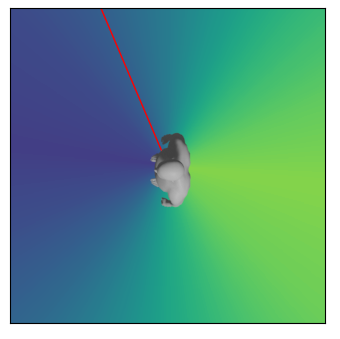
\includegraphics[width=0.24\linewidth]{pictures/transverseBench.png}}
	\subfloat[\centering Squat]{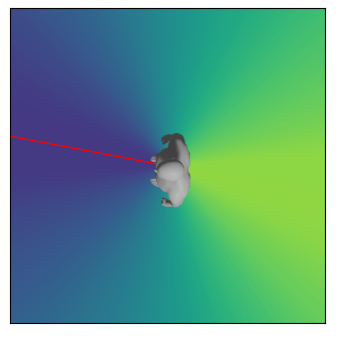
\includegraphics[width=0.24\linewidth]{pictures/transverseSquat.png}}
	\subfloat[\centering Bent-down]{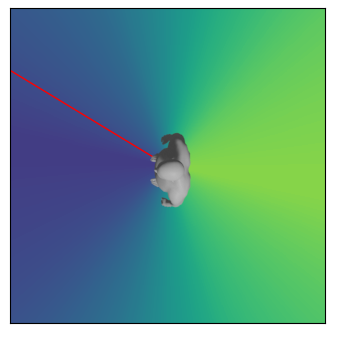
\includegraphics[width=0.24\linewidth]{pictures/transverseBend.png}}
	\subfloat[\centering Stand]{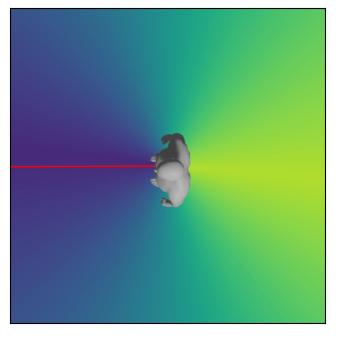
\includegraphics[width=0.24\linewidth]{pictures/transverseStand.png}}
\includegraphics[width=0.041\linewidth]{pictures/whitePixel.png}\\
	\subfloat[\centering Bench Press]{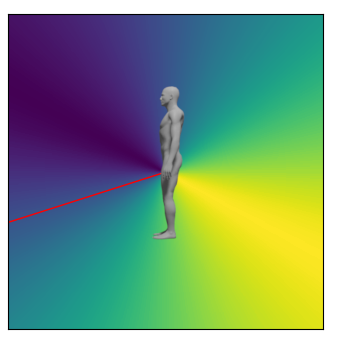
\includegraphics[width=0.24\linewidth]{pictures/medianBench.png}}
	\subfloat[\centering Squat]{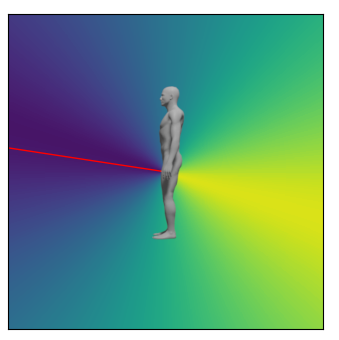
\includegraphics[width=0.24\linewidth]{pictures/medianSquat.png}}
	\subfloat[\centering Bent-down]{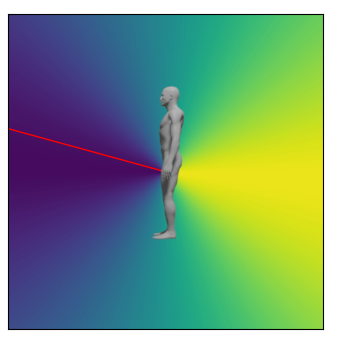
\includegraphics[width=0.24\linewidth]{pictures/medianBend.png}}
	\subfloat[\centering Stand]{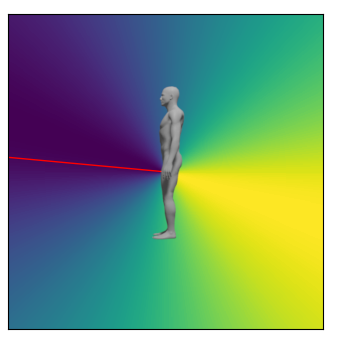
\includegraphics[width=0.24\linewidth]{pictures/medianStand.png}}    \includegraphics[width=0.041\linewidth]{pictures/scale.png}
	\caption{\emph{View Selection Error} (VSE) for different viewing angles from the top (a-d) and side (e-h) using the benchmark of Dutagaci et al.~\cite{dutagaci2010bbv}. The red line represents the view direction selected by our method. The human figure only shows spatial orientation and does not represent the executed movements.}
	\label{fig:colorMaps}
\end{figure*}

\section{Results\label{results}}
In \autoref{sec:results:selection}, we will discuss the performance of each algorithm's viewpoint selection relative to the user-selected viewpoints, using the method described in \autoref{sec:benchmark}. Subsequently, in \autoref{sec:results:analysis} the performance of the above-mentioned methods in optimizing viewpoints for the same exercise will be discussed, based on image sequences extracted from the videos. Lastly, \autoref{sec:results:comparison} concludes the user study results of the viewpoint comparison. The results of the questionnaire are found in \autoref{sec:study}, where they specify the participants, and in \autoref{sec:insights}, where the free-text answers are discussed.

\subsection{Viewpoint Selection \label{sec:results:selection}}
In \autoref{fig:colorMaps}, a low view selection error is represented by blue areas. Therefore, viewpoints in these areas aligned well with the user selection. Yellow areas were chosen less. The red line represents the viewpoint chosen by our method for the static pose without movement. Looking at \autoref{fig:colorMaps}, we see that our method calculated viewpoints predominantly lying in the blue regions, i.e., in regions preferred by users. Similarly, it becomes apparent when analyzing the view selection error mean over the four exercises, that, in comparison, our algorithm fits the selection of the users best with an average VSE of 0.3467. The static isometric-like view performed second best with an average VSE of 0.347 followed by JMO with 0.4825 and the method of Kwon et al. with 0.5497.

\subsection{Method Analysis\label{sec:results:analysis}}
To interpret the comparison of methods in \autoref{sec:results:comparison}, it is essential to understand the viewpoints each method provides and how these viewpoints change over time.

\textbf{JMO~\cite{ishara2015mra}:}
The JMO algorithm predominantly produced an adequate overview of the human body. A major drawback was that, when applied to videos, the algorithm erratically switched between viewpoints that were significantly distant from each other. This can be perceived in \autoref{fig:jmoSequence}. Consequently, the feedback often was difficult to comprehend, as the algorithm was not designed to work with visual cues or videos. Additionally, several viewpoints were selected from below and behind, although participants preferred perspectives from the front and slightly above (see \autoref{sec:results:selection}).

\textbf{Kwon et al.~\cite{kwon2020ocp}:} 
As can be seen in \autoref{fig:kwonSequence}, the algorithm of Kwon et al. seemed to predominantly produce views from behind in our application. As elaborated in \autoref{sec:results:selection}, this is a view that is mostly avoided by users. Additionally, the algorithm sometimes selected views from below, similar to the JMO algorithm mentioned earlier. The algorithm by Kwon et al. offered a much more stable perspective than JMO. However, the feedback was often challenging to see.

\begin{figure*}[h!]
	\centering
	\includegraphics[width=0.11\linewidth]{pictures/kwonSequence1.png}\hfill
	\includegraphics[width=0.12\linewidth]{pictures/kwonSequence2.png}\hfill
	\includegraphics[width=0.12\linewidth]{pictures/kwonSequence3.png}\hfill
	\includegraphics[width=0.12\linewidth]{pictures/kwonSequence4.png}\hfill
	\includegraphics[width=0.12\linewidth]{pictures/kwonSequence5.png}\hfill
	\includegraphics[width=0.12\linewidth]{pictures/kwonSequence6.png}\hfill
	\includegraphics[width=0.12\linewidth]{pictures/kwonSequence7.png}\hfill
	\includegraphics[width=0.115\linewidth]{pictures/kwonSequence8.png}\hfill
	\caption{Image sequence, taken from a video of a biceps curl exercise with deviation. The viewpoint is optimized by the algorithm by Kwon et al.~\cite{kwon2020ocp}.}
	\label{fig:kwonSequence}
\end{figure*}

\textbf{Ours:}
Our algorithm consistently transitioned between an optimal viewpoint for the neutral position and the contracted position with deviations, as illustrated in \autoref{fig:bicepsSequence}. When feedback was present, it was displayed clearly and perceivable emphasis on it. However, in some exercises, the rapid exercise execution caused a conflict between the neutral and the feedback-optimized viewpoint. This resulted in quick camera movements, which some users found irritating.

\subsection{Viewpoint Comparison \label{sec:results:comparison}}
\autoref{tab:comparison} shows the user choice distribution of the viewpoint comparison. Our algorithm was most prevalent with 35.04~\% of votes, the isometric-like position was chosen second most with 32.48~\%, followed by Kwon et al.~\cite{kwon2020ocp} with 17.52~\% and lastly JMO~\cite{ishara2015mra} with 14.96~\%.

\begin{figure*}[h]
	\centering
	\includegraphics[width=0.11\linewidth]{pictures/jmoSequence1.png}\hfill
	\includegraphics[width=0.12\linewidth]{pictures/jmoSequence2.png}\hfill
	\includegraphics[width=0.12\linewidth]{pictures/jmoSequence3.png}\hfill
	\includegraphics[width=0.10\linewidth]{pictures/jmoSequence4.png}\hfill
	\includegraphics[width=0.12\linewidth]{pictures/jmoSequence5.png}\hfill
	\includegraphics[width=0.12\linewidth]{pictures/jmoSequence6.png}\hfill
	\includegraphics[width=0.12\linewidth]{pictures/jmoSequence7.png}\hfill
	\includegraphics[width=0.12\linewidth]{pictures/jmoSequence8.png}\hfill
	\caption{Image sequence, taken from a video of a biceps curl exercise with deviation. The viewpoint is optimized by the \emph{Joint Mutual Occlusion} algorithm by Ishara et al.~\cite{ishara2015mra}.}
	\label{fig:jmoSequence}
\end{figure*}

\begin{figure*}[h]
	\centering
	\includegraphics[width=0.115\linewidth]{pictures/bicepsSequence1.png}\hfill
	\includegraphics[width=0.13\linewidth]{pictures/bicepsSequence2.png}\hfill
	\includegraphics[width=0.125\linewidth]{pictures/bicepsSequence3.png}\hfill
	\includegraphics[width=0.125\linewidth]{pictures/bicepsSequence4.png}\hfill
	\includegraphics[width=0.12\linewidth]{pictures/bicepsSequence5.png}\hfill
	\includegraphics[width=0.115\linewidth]{pictures/bicepsSequence6.png}\hfill
	\includegraphics[width=0.11\linewidth]{pictures/bicepsSequence7.png}\hfill
	\includegraphics[width=0.11\linewidth]{pictures/bicepsSequence8.png}\hfill
	\caption{Image sequence, taken from a video of a biceps curl exercise with deviation. The viewpoint is optimized by our algorithm.}
	\label{fig:bicepsSequence}
\end{figure*}

Occasionally camera positions from behind were provided by the methods of Kwon et al.~\cite{kwon2020ocp} and Ishara et al.~\cite{ishara2015mra}. Additionally, they produced an unsteady camera movement, because they jumped between far-distant viewpoints and generally, had just a limited amount of viewpoints available. In contrast, the static isometric-like viewpoint produced surprisingly good results, although it lacked an adaptation for movement or feedback. The primary advantage of the isometric-like viewpoint over the other methods was its stability. Our method provided an adequate view of the neutral positions of the exercises. Furthermore, it produced a continuous camera movement toward a feedback-oriented viewpoint with increasing deviation. However, the camera movement showing the bench press and bent-over row exercises was occasionally rapid.

\section{Insights and Discussion\label{sec:insights}}
Looking at \autoref{fig:colorMaps}, it becomes evident that the participants preferred a frontal view direction. This aligns with the statement made by Zusne~\cite{zusne1970vpf}, that humans desire frontal views (see \autoref{sec:considerations}), and verifies these requirements for our application. Additionally, it was observed that participants preferred a viewpoint from slightly above.

\begin{table}[h]
	\caption{\label{tab:comparison}Results of user study. Distribution of viewpoint selection methods chosen by the participants.}%
	\begin{tabular}{@{}l|llllll|l@{}}
		\toprule
		Method & \begin{sideways}Bench press\end{sideways} & \begin{sideways}Biceps curl A  \end{sideways} & \begin{sideways}Lateral raises\end{sideways} & \begin{sideways}Shoulder press\end{sideways} & \begin{sideways}Bent-over row\end{sideways} & \begin{sideways}Biceps curl B\end{sideways}  & \begin{tabular}{l}Total\\Percentage\end{tabular} \\
		\midrule
		Neutral  & 19 & 15 & 3 & 15 & 6 & 18 & 32.48 \% \\
		JMO & 1 & 1  & 6  & 0 & 25 & 2 & 14.96 \% \\
		Kwon & 14 & 7  & 3  & 3 & 6 & 8 & 17.52 \% \\
		Ours  & 5 & 16 & 27  & 21 & 2 & 11 & \textbf{35.04 \%} \\
		\bottomrule
	\end{tabular}
\end{table}

Our algorithm performs significantly less well for some specific exercises. This can be attributed to the consistently smooth, though occasionally rapid, camera movement. In particular, the camera moved rapidly during the bench press and bent-over row exercises. As stated in \autoref{sec:methViewCalc}, our algorithm generally prevents inconsistent camera movement, though rapid camera motions may still occasionally occur.

The most prevalent statement made by the participants regarded the camera movement consistency. Specifically, users were irritated by movements that were too rapid or erratic. This observation matches the findings by Assa et al.~\cite{assa2008moh} concerning camera paths. Additionally, many participants indicated that having multiple camera perspectives would help them to understand the poses and feedback. This is especially interesting for future work and when applying suggested methods. Additionally, some users desired the option to select no method, as they felt none of the suggested perspectives were adequate. This implies that there are possible improvements to our algorithm and that human viewpoint preferences might need further assessment. Lastly, some users struggled to interpret poses without relation to the environment. Primarily, this concerned the bench press exercise, where a virtual bench might help users interpret the avatar posture. Therefore, incorporating the surrounding environment could enhance understanding, especially for exercises involving equipment such as weights, benches, and pull-up bars. However, additionally rendered equipment could occlude the avatar or visual cues and therefore hinder the perception of the provided feedback.

The spatial registration (see \autoref{sec:methReg}) for our use case was trivial, since the superimposed exercises were recorded at the same position with the same individual. Other circumstances, like varying individuals or different registration methods can yield fundamentally different results in terms of feedback appearance. However, the view selection methods, as presented in \autoref{sec:methViewCalc}, would still find a valid viewpoint. Depending on what registration methods were chosen, the view selection could be skewed toward the feedback deviation. If there are other registration methods chosen, it might be necessary to adapt the constants in the viewpoint selection calculation (in particular, $w$ and $\delta_0$ in \autoref{eq:viewpoint}) to retrieve the desired perspectives.

\section{Conclusion}
The chapter at hand provides novel insights on how to optimize the display of superimposed avatars. As we can see in current literature, the superimposition of avatars plays an increasingly important role. As an accessible and intuitive method of providing and receiving motor feedback, it is widespread in both mixed reality and traditional feedback technologies.

The consideration of avatar registration is inevitable when attempting to optimize the display of superimposed avatars. In the literature, avatars are often registered by aligning the position and/or rotation of a single joint. For specific use cases, this can be adequate. However, to ensure that users can easily understand a wide range of exercises, a more detailed approach must be taken. We offer valuable insights on how certain exercises could be optimally registered based on the performed exercise. Without the claim for completeness, we offer fundamental guidelines as the basis for application development or further research. Furthermore, we provide concrete examples to help with comprehension and potential implementation.

Avatar registration, important by itself, additionally represents a major factor of influence on viewpoint selection, another essential topic for optimal display of superimposed avatars. We introduce a new method for selecting viewpoints for motor feedback, such as superimposed avatars, among other options. Not only is this method computationally faster than the methods found in the literature, but evaluation in the context of a user study showed, that participants preferred our method over other methods found in the literature.

Our registration and viewpoint selection methods combined can adequately optimize the display of superimposed avatars. However, the individual methods provide value as well, as they can be utilized separately from each other.
\externaldocument{content/survey}
\externaldocument{content/registration}
\chapter[Omnipresent In-Situ Feedback for Motor Skill Training using AR]{Omnipresent In-Situ Feedback for Motor Skill Training using Augmented Reality \label{chap:omnipresent}}
According to the World Confederation for Physical Therapy, 1,962,741 physical therapists practiced worldwide in 2023. Europe in particular had the highest rate of physiotherapists with 13.5 per 10,000 people~\cite{worldphysiotherapy2023global}. This may be attributed to the fact that 20\% of people globally suffer from chronic pain \cite{treede2015classification}. With computer science advancing, technology can increasingly support therapists and clients alike during therapy. For instance, superimposing virtual content onto the user's perception, as common in \acrshort{mr}, can assist during physical therapy or exercise to facilitate the correct execution of motion \cite{brepohl2023virtual},\cite{campo2021immersive},\cite{diller2022vcb}.

Throughout the literature, we see the use of \acrshort{hmd}s to provide feedback for physical therapy and exercise. On the one hand, these technologies present many challenges to overcome. For example, the first-person perspective of \acrshort{hmd}s limits the user’s view of the user's body parts. On the other hand, \acrshort{hmd}s offer solutions to problems that occur, when providing visual feedback during physical therapy and exercise. For instance, providing visual feedback in a manner that allows users to maintain a neutral head position is challenging. However, if the feedback can only be perceived on a wall-mounted display, users are forced to change their head position, and this --- in the worst case --- inhibits the execution of the correct movements. This can bear serious consequences, such as becoming accustomed to incorrect exercise movement, possibly even leading to injury. For instance, when executing squats correctly, the spine is meant to stay straight. Feedback provided on an \acrshort{rmd} can force the user to bend or twist the neck (and with it the spine) to see the feedback. Therefore, the exercise becomes uncomfortable, the execution can become incorrect, and thus the risk of injury can increase --- especially when performing the exercise with free weights (e.g. barbell). Alternatively, if the exercise is executed correctly and securely, the feedback via \acrshort{rmd} might not be in the user's field of view.

When the motion feedback is provided via an \acrshort{hmd}, the user can execute the movements correctly, comfortably, and non-injuriously. Since the display is mounted on the head, the visual cues can adapt to the head position and the view direction and thus be omnipresent. In this chapter, we present the novel approach \emph{SkillAR} to provide such omnipresent, in-situ, and corrective feedback (as specified in \autoref{sec:feedback}), which adapts to the user's movements, and hence can facilitate an organic and healthy exercise performance. Additionally, we present the results of a user study verifying that SkillAR has no additional disadvantages compared to a conventional screen.

\section{Point of View in Motor Feedback\label{sec:omnipresent:POV}}
Considering motion feedback, the \emph{\acrshort{pov}} plays an important role. A first-person perspective (\autoref{fig:POV:AR}, right) provides an immersive and natural viewpoint, as we usually experience the world from this angle. However, the foreshortening deriving from this perspective can make it difficult to perceive the spatial positioning of limbs. Furthermore, some body parts, like the back, can simply not be observed from this limited viewpoint. 
Optical see-through \acrshort{hmd}s (as are used in this chapter) always provide a natural first-person perspective in addition to any other superimposed feedback types.

Alternatively, a common way to display motion feedback is a third-person perspective (\autoref{fig:POV:AR}, left). This gives the user an overview of his or her body in space. The relation of all limbs becomes clear and deviations from the correct form can be adjusted accordingly. Therefore, Rymal and Ste-Marie~\cite{rymal2009dsm} discovered that an exocentric view of an exercise could help athletes improve their ability to mentally visualize the motion, which can lead to learning new skills or improving performance~\cite{white1998ida}. Moreover, we elaborated in \autoref{chap:visualCueSurvey} that a third-person view is predominantly used in current literature when providing visual feedback for motor skills.

\begin{figure*}[b!]
	\centering
	\includegraphics[width=0.49\linewidth]{pictures/ExocentricAR.jpg}\hfill
	\includegraphics[width=0.49\linewidth]{pictures/EgocentricAR.jpg}
	\caption[Examples of exocentric and egocentric motion feedback in \acrshort{ar}.]{Examples of exocentric (left) and egocentric (right) motion feedback in augmented reality. The possible target movement is in both cases represented by a green avatar. Compare to the stylized illustration in \autoref{fig:POV}.}
	\label{fig:POV:AR}
\end{figure*}

Furthermore, for facilitating a user-friendly and intuitive viewpoint selection \autoref{sec:considerations} provides additional considerations. Moreover, with the methods presented in \autoref{sec:methViewCalc}, it is possible to calculate an optimized viewpoint of the exocentric motion feedback. However, this exceeds the scope of this chapter.

\section{Common Visual Feedback Technologies} %Methods?
The most common tool to obtain a full-body view (i.e. third person / exocentric as seen in \autoref{fig:POV:AR} and explained in~\autoref{sec:omnipresent:POV}) is the mirror. Ballet dancers and their instructors have utilized mirrors to acquire simple visual feedback since the 19th century~\cite{desmond1997mim}. Likewise, mirrors are to be found in fitness studios and physiotherapy studios all over the world. Furthermore, it is possible to enhance the natural feedback of the mirror with technology. Such enhancements often lead to smart mirrors, which can assist with correct exercise execution (e.g. \cite{kim2020rtm}, \cite{park2021ued}). Moreover, some approaches use the mirror metaphor in a \acrshort{vr} setting to create an intuitive feedback system (e.g. \cite{waltemate2016tlp}, \cite{huelsmann2019ssp}). These so-called \emph{virtual mirrors} are additionally often used to increase the sense of embodiment \cite{inoue2021virtual}, \cite{gonzalesfranco2010contribution}.

Equally important in recent research are conventional displays. Especially in connection with mobile devices or computers, displays are able to provide visual feedback for motor skill training. In some instances, \acrshort{rmd}s mimic the function of mirrors. These approaches are commonly described as \emph{augmented mirrors}. For example, Anderson et al.~\cite{anderson2013youmove} visualize an actual avatar and a target avatar on a room-scale display in addition to a camera stream. Likewise, Trajkova et al.~\cite{trajkova2018ttb} provide feedback as a mirrored camera stream with superimposed feedback. As we showed in \autoref{chap:visualCueSurvey}, augmented mirrors are a prevalent motor feedback approach in the literature. 

\section{Related Work}
Several approaches addressed the limitations of the first-person perspective in \acrshort{hmd}s as described in \autoref{sec:omnipresent:POV} when providing motion feedback. For example, Chua et al. \cite{chua2003tpt} provided feedback for tai chi displaying several redundant exocentric feedback avatars around the user. This solved the visibility issue when moving the head, i.e. changing the view direction in the first-person perspective in \acrshort{vr}. Additionally, the approach explored different feedback methods, like a single teacher or superimposed wireframe feedback.

Likewise, Han et al. \cite{han2017mtc} utilized multiple coaches fixed in space and oriented circularly around the user. However, they transferred the idea into \acrshort{ar}. In addition to the redundant instructors (see also \autoref{sec:instructor}), a drone was automatically navigated to record the user. This video stream was then displayed in \acrshort{ar}, mimicking a mirror. As a result, the user could see a coach executing the target movement in every horizontal direction juxtaposed with the mirror image. However, while this approach might be well-matched for the use case of tai chi, feedback would not be visible in exercises where the view is naturally directed to the ground (e.g. planks, push-ups) or the ceiling (e.g. sit-ups, bench press).

Yan et al.~\cite{Yan2015oma} solved the issue of a limited first-person perspective by juxtaposing the \acrshort{hmd} video pass-through with the video stream of an external camera. This image was cropped at the silhouette to blend with the surroundings and create a cohesive \acrshort{mr} experience. Although the approach provided an exocentric feedback of the body, the functionality was limited by the position and view direction of the physical camera.

In contrast to the previously mentioned works, Kawasaki et al.~\cite{kawasaki2010cst} included the perspective of another person by superimposing the user's view with the video see-through stream of an \acrshort{hmd}. As a result, the user could see if his or her motions corresponded with the instructor's. This enabled skill transmission in a user study. A similar approach was taken by Kasahara et al.~\cite{kasahara2016pe}, who also included another person's perspective in an \acrshort{hmd}. In contrast to the previous work, the two perspectives were juxtaposed. The two approaches enhance the egocentric perspective, therefore they are well suited for skill training mostly involving the hands, like diabolo juggling~\cite{kawasaki2010cst} or drawing~\cite{kasahara2016pe}. However, they lack an exocentric perspective and hence an overview of the body, making feedback for whole-body exercises impossible.



In addition, Ikeda et al. \cite{ikeda2018arb} displayed stationary small-scale (1:4) avatars in real-time during the motion and true-scale models during playback feedback. As the system was built specifically for golf swings and players look downwards during swings, the small-scale avatar could be seen during the exercise performance. Afterward, when replaying a recorded exercise, the view was no longer restricted by the exercise. Consequently, the avatar was displayed in true-scale. Although the avatar could be seen well when performing a golf swing, there are some exercises, for which providing feedback with this system would prove difficult. In particular, difficulties arise for exercises where rotating the view direction on the horizontal plane or an almost vertical view direction is necessary.

Lastly, Hamanishi et al. \cite{Hamanishi2019avu} developed a system that enables the user to view his or her motions from all sides. This was achieved by giving the motion-captured avatar a fixed direction in space. Consequently, the user can walk around it, viewing it comprehensively. The two participants of the qualitative user study seemed to receive the system well. However, it might not be sufficient for all forms of exercise. For example, the feedback might irritate users during exercises where the view direction changes a lot (e.g. sit-ups, torso rotations). Furthermore, the system did not provide a target movement for the user to imitate. Hence, the system does not qualify as \emph{corrective feedback} (see \autoref{sec:feedback}), which is the focus of the work at hand.

\section{Omnipresent Feedback}
This section will explain the SkillAR system in detail. First, \autoref{sec:overview} and \autoref{sec:register} will provide information about the hardware used and the nature of the feedback displayed. This should give the reader an understanding of the whole system. Our main contributions lie in the combination of methods found in \autoref{sec:transformation} to ensure the omnipresence of the feedback.

\subsection{System Overview \label{sec:overview}}
\begin{figure}[b!]
	\centering
	\includegraphics[width=\linewidth]{pictures/HoloLensScreenshot.jpg}
	\caption[Screenshot of the motor feedback provided by SkillAR via \acrshort{hmd}.]{Screenshot of the egocentric motor feedback provided by SkillAR via \acrshort{hmd}. \label{fig:screen}}
\end{figure}
In order to provide visual feedback for motions and in particular exercises, it is necessary to capture the limb positions in space over time. For this reason, we used a 3D camera, which extracted joint coordinates from a recorded point cloud. Consequently, a skeleton-like avatar as seen in \autoref{fig:screen} could be constructed on the \acrshort{hmd}, showing the executed motion in real-time. In addition to the current motion, we superimposed a recorded movement, which represents an ideal execution of the movement. As a result, the user can now correct the motion following the provided feedback. In addition to superimposition, there are further possibilities to display comparative visuals as analyzed by L'Yi et al.~\cite{lyi2021comparative}. Varying avatars and visual cues could impact how users perceive the feedback and therefore yield different results in a user study as conducted in \autoref{sec:evaluation}. However, evaluating different visual cues and avatars would exceed the scope of this paper.


\subsection{Avatar Registration \label{sec:register}}
As described in \autoref{chap:registration}, the registration of superimposed avatars is no trivial subject. Depending on where the actual and target avatars are registered, the visualization is perceived as intuitive or irritating by the user.
\begin{comment}
\begin{figure*}[h!]
	\centering    \subfloat{\includegraphics[width=0.5\linewidth]{pictures/pelvisRegistration.png}\hfill}
	\subfloat{\includegraphics[width=0.5\linewidth]{pictures/footRegistration.png}\hfill}
	\caption[Example of different methods registering squatting skeletons.]{The reference (in green) is performing the ideal exercise --- in this case a squat --- while the actual avatar is neutrally standing. The result of registering at the pelvis (left) looks as if hovering and can potentially be irritating to the user. In this case, it might be preferable to register the avatars at the foot or the ground. \label{fig:registration}}
\end{figure*}
\end{comment}


\begin{figure*}[t!]
	\centering
	\subfloat[\centering Standing]{\includegraphics[width=.13\linewidth]{pictures/Standing.png}\hfill}  
	\subfloat[\centering Jumping\\Jack]{\includegraphics[width=.15\linewidth]{pictures/JumpingJack.png}\hfill} 
	\subfloat[\centering Plank]{\includegraphics[width=.15\linewidth]{pictures/Plank.png}\hfill} 
	\subfloat[\centering Squat]{\includegraphics[width=.15\linewidth]{pictures/Squat.png}\hfill} 
	\subfloat[\centering Torso\\Rotation]{\includegraphics[width=.13\linewidth]{pictures/TorsoRotation.png}\hfill}
	\subfloat[\centering Warrior II]{\includegraphics[width=.22\linewidth]{pictures/WarriorII.png}\hfill} 
	\caption{Example exercises with deviations as described in \autoref{sec:design}.}
	\label{fig:exercises}
\end{figure*}

Consequently, in our work, we fixated the actual avatar and matched the horizontal position of the pelvises. For the vertical position of the target reference avatar, we matched the lowest feet position of both avatars, considering that it should be on the ground since we did not include exercises that involved jumping or hanging (see~\autoref{fig:exercises}), as we wanted the exercises to be feasible for a large group of people. Considering rotation, the orientation of the actual pelvis joint was transferred to the target pelvis joint. The registration methods closely align with the approach presented in \autoref{chap:registration}. For an in-depth analysis of avatar registration, see the corresponding chapter.

Additionally, the target avatar had to be scaled bone-wise to match the anatomy of the user. Otherwise, it would be impossible for the user to mimic poses recorded by someone else, as limbs cannot be stretched or compressed. If the same individual records the ideal and actual execution, this step can be skipped. Furthermore, the avatars were mirrored horizontally, as this makes it easier to take the displayed pose and increases embodiment as stated, for example, by Raffe and Garcia~\cite{raffe2018combining}.

\subsection{Feedback Transformation \label{sec:transformation}}
Because SkillAR intends to provide omnipresent in-situ feedback, avatar transformation in space is crucial. Utilizing the orientation of the \acrshort{hmd} in space and the information we have of the body and surroundings, we can transform the feedback to adapt to the head movement during different exercises and to facilitate a better understanding of the feedback itself. Internal pilot studies have shown various important aspects that we will illustrate in the following.

\textbf{Placement:}
The stereoscopic display of the \acrshort{hmd} makes it possible for the user to perceive the avatars in space. Consequently, placing the avatars in relation to the actual surroundings of the users helps enhance the interpretation of the feedback. For this purpose, we use the view direction $\vec{v}$ of the \acrshort{hmd} to place the avatar. An intuitive way of placing would be to position the avatars' feet at the intersection of $\vec{v}$ with the floor plane. However, this would often lead to the avatar only taking up the upper half of the user's field of view. Instead, the avatars' pelvis represents an adequate approximation of the body center. Yet, we can not place the avatar with its pelvis is at floor height, as the feedback would appear too low (partially below ground) and hence be irritating. Instead, we constructed a plane $P$ horizontally through the user's pelvis. The avatars (registered as described in \autoref{sec:register}) were then positioned by placing the pelvises at the intersection of $\vec{v}$ and $P$ as seen in~\autoref{fig:positioning}. Using the pelvis orientation as an indicator for the forward direction of the avatar, the feedback was rotated around the vertical axis, so it faced the virtual camera and thus, the user. This supports the mirror metaphor and hence user guidance as described in~\autoref{sec:register}. The steps above ensure that the feedback is visible in any view direction, i.e. omnipresent.

\begin{figure}[b!]
	\centering
	\includegraphics[width=0.6\linewidth]{pictures/avatarPos.png}
	\caption[Positioning of the feedback avatar.]{The feedback avatar is positioned such that its pelvis lies on the intersection of the view direction $\vec{v}$ and the horizontal plane through the user's pelvis $P$.\label{fig:positioning}}
\end{figure}

\textbf{Snapping:}
While moving --- especially during exercises --- the head movement can be unstable, leading to an erratic feedback placement. Consequently, the visual feedback becomes irritating for the user. Therefore SkillAR only moves the feedback if the intersection of $\vec{v}$ with $P$ exceeds a certain distance $\Delta$ from the current avatar position as seen in~\autoref{fig:roundGrid}. The feedback is moved smoothly to its new position, which leads to a far more stable system behavior similar to snapping.

\begin{figure}[t!]
	\centering
	\includegraphics[width=0.6\linewidth]{pictures/gridRound.png}
	\caption[Spatial stabilization of the feedback positioning.]{The avatars move horizontally if the view direction deviates more than $\Delta$ from the center of the visualization, as indicated by the circles. The visualization is scaled up in the distance and down in proximity to the camera. The constant size always matches the field of view of the \acrshort{hmd} and irritates the user less as if it were constantly changing.\label{fig:roundGrid}}
\end{figure}

\textbf{Scaling:}
Moreover, the size of the feedback is scaled depending on the distance to the virtual camera to optimally utilize the \acrshort{hmd}'s field of view.  This is illustrated in~\autoref{fig:roundGrid}. Likewise, the snapping threshold $\Delta$ is scaled (also visible in~\autoref{fig:roundGrid}) to facilitate a consistent user interaction. Scaling the avatar results in slightly contradicting depth cues: The vergence changes with the distance, but the size stays constant due to the scaling. Additionally, the avatars are still appropriately located in the scene, but they might no longer connect with the real floor plane. However, it is to be said, that our priority is to provide omnipresent in-situ feedback rather than creating a perfectly immersive experience. None of the users commented about the above-mentioned topics (see \autoref{sec:comments}).

\textbf{Top-Down Mode:}
When looking down, the feedback positioning at pelvis height becomes hard to perceive as it appears too close. This would prevent the user from perceiving feedback when doing exercises that involve a downward head orientation like planks or push-ups. For this reason, when the angle $\gamma$ between the view direction $\vec{v}$ of the \acrshort{hmd} and the vertical axis lies below 20° (see in~\autoref{fig:floor}), SkillAR displays the feedback in a constant distance below the user (underneath the physical floor plane). In this top-down view, the avatars are facing the same way as the user and are not mirrored. This provides an overview of exercises facing down, allowing for an \acrshort{ar}-supported execution of, for example, push-ups.

\begin{figure}[h!]
	\centering
	\includegraphics[width=0.6\linewidth]{pictures/floorPos.png}
	\caption[Top-down mode visualizing exercises when looking down.]{The feedback transitions to a \emph{top-down mode}, in which the avatars are shown below, if the angle $\gamma$ between the normal of the floor and the view direction is smaller than 20°. \label{fig:floor}}
\end{figure}

\textbf{Free Mode:}
Likewise, the feedback positioning mode changes when looking upwards. In this case, the avatars can not be placed at the intersection of $\vec{v}$ and $P$ as they no longer intersect. Consequently, the avatar positioning is then strictly bound to the view direction. The distance to the camera is constant, and the avatar still faces the user. While the avatar's relation to its environment is less clear in this mode, it allows for performing exercises with an upward-facing view direction like sit-ups or bench press.

\section{Evaluation}
SkillAR provides major advantages for viewing motor feedback: Users can view the ideal form while performing exercises without compromising comfort, good form, or safety. We conducted a user study to verify that SkillAR has no additional major disadvantages compared to a conventional \acrshort{rmd}. This study was reviewed by the ethics committee and the data protection official of the University of Applied Sciences Worms and carried out following the appropriate guidelines and regulations. Consequently, the participants were informed upon invitation about the legal circumstances and anonymity of the study. Only the following data was recorded: Age, gender, vision deficiencies, and affiliation with the university. It is not feasible, that they lead to identifying a person's identity. Therefore, written consent was not necessary according to the ethics committee and data security office. \acrshort{usb} drives and sunglasses were offered as compensation.

\subsection{Participants}
For the user study, 32 individuals were recruited from an academic environment. Their age ranged from 22 to 61 (\(\mathrm{M} = 35.4, \mathrm{Mdn} = 30.5, \mathrm{SD} = 11.1\)). Their gender was evenly distributed among males and females with 16 (\(50.0\%\)) individuals each. They rated their prior \acrshort{xr} experience on a scale from one to five, with one equaling no previous engagement in \acrshort{xr} and five being an \acrshort{xr} expert. The rating averaged out at 1.8 (\(\mathrm{M}=1.8, \mathrm{Mdn} = 1.75, \mathrm{SD} = 0.9\)) and their physical activity at 3.1 (\(\mathrm{M}=3.1, \mathrm{Mdn} = 3, \mathrm{SD} = 0.9\)) (one again representing no physical activity and five the maximum). As the visual capabilities of individuals play an important role in the study, the number of participants wearing glasses (\(\mathrm{n} = 17, \mathrm{i.e.}~53.1\%\)) was documented as well as visual impairments: Three participants (\(9.4\%\)) reported to have limited or missing spatial perception. One participant exhibited both red-green and blue-yellow color vision deficiency. Regarding gender, the participants' demographics match the population of Europe and the world well. The median age of the participants lies between the median age of Europe (\(42.2\)) and the world (\(30.4\)) as estimated by the \acrshort{un} in 2023~\cite{united2022world}. However, the educational background is expected to be higher than average in our user group, as the individuals were recruited in an academic environment.


\subsection{Apparatus}
A Microsoft Azure Kinect 3D camera provided the spatial positions of the joints. It was set up on a tripod about 2,5 m from the subject to ensure that everything was in frame. The visualization and experimental applications were developed in Unity. To display the augmented reality sections of the study a Microsoft HoloLens 2 was utilized. Additionally, to ensure the legibility on the HoloLens, the blinds in the room were closed to provide consistent lighting conditions for the participants. Internal pilot studies showed, that it is hard to perceive the visualization in intensely illuminated environments.

It was ensured the participants understood the avatars, the visual feedback, and the study tasks beforehand. The study took a total of about 20 min with 5 min of introduction. Every task demanded approximately the same duration. Exercises could be skipped or aborted at any time due to health concerns.

\subsection{Tasks \label{sec:tasks}}
In the \textbf{comparison} task, the user was asked to identify errors represented by an actual and a target avatar as seen in \autoref{fig:exercises}. The answers were documented and categorized, regarding the accuracy of the addressed body part and correction. With both --- the body part and the correction --- being able to be either correct or incorrect, this led to $2 \times 2$ categories. It was possible for answers to fall into several categories, as sometimes participants made contradicting remarks or answered both correctly and incorrectly successively. Additionally, the time to answer was measured. This task was carried out using the \acrshort{hmd} and the \acrshort{rmd} sequentially.

The \textbf{imitation} task involved the users mimicking a pose they saw superimposed with their actual pose on the \acrshort{hmd} or \acrshort{rmd}. After adapting the pose, they gave a command, and the distances of joints, and the time elapsed since the display started showing the pose, were recorded. In between the exercises, no feedback was visible, and the users could retake a neutral position and recover from the previous exercise. This should prevent impacting the following exercise performances in any way (e.g. adding time, because the participant has to stand up after an exercise on the ground). This task was carried out using the \acrshort{hmd} and the \acrshort{rmd} sequentially.

Finally, the participants answered structured \textbf{questions} regarding their demographic including age, affiliation, XR experience, physical activity, optical deficiencies, gender, and potential comments.

\subsection{Study Design \label{sec:design}}
The study aimed to compare SkillAR to conventional \acrshort{rmd}s using an in-subject design measuring time and accuracy during the comparison and identification tasks. A few border case exercises were selected, representing various body positions in space. In addition, deviations were chosen to be evaluated during the comparison task (see below) to evaluate the feedback interpretation. These deviations require corrections in different directions to correct: Bend vertically, tilt side-wards, raise or lower limbs, twist, etc. Furthermore, the following exercises were each represented by a still pose: Standing, jumping jack, plank, squat, torso rotations, and warrior II as found in yoga. These exercises can be seen including the deviations from the ideal in \autoref{fig:exercises}. The order of exercises, tasks, and devices was randomized to eliminate any learning bias. Moreover, the intent of the study was not to evaluate how well an exercise was executed, but how well the feedback could be comprehended.

In the \textbf{comparison} task, users were asked to identify errors represented by an actual and a target avatar as seen in \autoref{fig:exercises}. The answers were documented and categorized, regarding the accuracy of the addressed body part and correction. With both --- the body part and the correction --- being able to be either correct or incorrect, this led to $2 \times 2$ categories. It was possible for answers to fall into several categories, as sometimes participants made contradicting remarks or answered both correctly and incorrectly successively. Additionally, the time to answer was measured. This task was carried out using the \acrshort{hmd} and the \acrshort{rmd} sequentially.

The \textbf{imitation} task involved the users mimicking an ideal pose they saw superimposed with their actual pose on the \acrshort{hmd} or \acrshort{rmd}. After adapting the pose, they gave a command, and the distances of joints, and the time elapsed since the display started showing the pose, were recorded. In between the exercises, no feedback was visible, and the users could retake a neutral position and recover from the previous exercise. This should prevent impacting the following exercise performances in any way (e.g. adding time, because the participant has to stand up after an exercise on the ground). This task was again carried out using the \acrshort{hmd} and the \acrshort{rmd} sequentially. The supplemental material provides a video of the juxtaposed exocentric and egocentric perspectives of a user imitating poses.

Finally, the participants answered structured \textbf{questions} regarding their demographic including age, affiliation, \acrshort{xr} experience, physical activity, optical deficiencies, gender, and potential comments.

\section{Results}
We suspected a dependency between \acrshort{rmd} and \acrshort{hmd} regarding the results of the same tasks. Additionally, we had no assumption which device would allow for more accuracy or a faster task completion time. Consequently, a dependent two-tailed t-test seemed most appropriate to evaluate the results. For this purpose, the results of one individual were averaged, so they were comparable during the test. One evaluation of the comparison task was discarded, as it was not suitable for evaluation due to technical difficulties leading to an incomplete recording. For the t-test, we assumed a significance level of \(\mathrm{\alpha} = 0.05\).

\subsection{Completion Time Analysis}
During each of the study tasks, the time to completion was measured. In particular, the time from the start of displaying the exercise to identifying the exercise or adopting the displayed pose. When imitating poses, this was starting from a neutral standing pose.

\begin{table}[b!]
	\caption{Time measurements for each task in the user study.}\label{tab:time}
	\begin{tabular*}{\textwidth}{@{\extracolsep\fill}lcccccc}
		\toprule%
		& \multicolumn{2}{@{}c@{}}{Comparison} & \multicolumn{2}{@{}c@{}}{Imitation} \\\cmidrule{2 - 3}\cmidrule{4-5}%
		Device & \acrshort{rmd} & SkillAR & \acrshort{rmd} & SkillAR \\
		\midrule
		Mean  & 18.81 s & 19.01 s & 21.42 s & 22.95 s\\
		Median & 14.70 s  & 17.95 s  & 19.94 s & 22.43 s\\
		Standard Deviation  & 11.44 s & 8.17 s & 7.78 s & 7.80 s\\
		\bottomrule
	\end{tabular*}
\end{table}

Regarding the comparison task, SkillAR exhibits an insignificantly (\(\mathrm{p}=0.92\)) longer time to assess the feedback while featuring a lower standard deviation, as seen in \autoref{tab:time}. Likewise, the users required an insignificantly (\(\mathrm{p}=0.38\)) longer time to mimic the poses displayed with SkillAR compared to the \acrshort{rmd}.

\subsection{Accuracy Analysis}
In the comparison task, the percentage of right answers (right body part and right correction) was recorded per user per device. When measuring the accuracy of the pose imitation, we measured the distance of each joint to its counterpart in the ideal pose. These were then averaged to find the mean deviation of the user pose per device.

Assessing the accuracy in the comparison task between the \acrshort{rmd} and SkillAR, we see
that users could identify the corrections significantly (\(\mathrm{p}=6 \cdot 10^{-7}\)) more precisely with SkillAR in relation to a conventional \acrshort{rmd}. As in this case the p-value is far smaller than $\alpha$, it seems likely that SkillAR facilitates a more precise interpretation of the given feedback. When imitating the poses, the precision was insignificantly (\(\mathrm{p}=0.37\)) higher using the \acrshort{rmd} compared to SkillAR.


\begin{table}[b!]
	\caption{Accuracy for each task in the user study.}\label{tab:accuracy}
	\begin{tabular*}{\textwidth}{@{\extracolsep\fill}lcccccc}
		\toprule%
		& \multicolumn{2}{@{}c@{}}{Comparison} & \multicolumn{2}{@{}c@{}}{Imitation} \\\cmidrule{2 - 3}\cmidrule{4-5}%
		Device & \acrshort{rmd} & SkillAR & \acrshort{rmd} & SkillAR \\
		\midrule
		Mean  & 75.27 \% & 92.71 \% & 10.71 cm & 11.14 cm\\
		Median & 83.33 \% & 100.00 \% & 10.17 cm & 10.82 cm\\
		Standard Deviation  & 11.88 \% & 12.46 \% & 2.56 cm & 3.33 cm\\
		\bottomrule
	\end{tabular*}
\end{table}

\section{Discussion}
In the statistical analysis, we could not verify a significant difference between SkillAR and \acrshort{rmd} regarding the comparison time as well as time and accuracy when mimicking poses. The large standard deviation compared to the mean suggests that an even more controlled study with more participants and a more precise camera could be profitable. Further, the measurements of the two analyzed methods seem quite similar. It might be profitable to analyze the statistical equivalence of the methods in future studies. However, our evaluation shows that the participants identify the right feedback significantly more often with SkillAR compared to an \acrshort{rmd}. The mean difference is large compared to the standard deviation. We attribute this mainly to the fact, that it is possible to perceive a 3D image of the feedback with the \acrshort{hmd}: Due to the two displays in the \acrshort{hmd}, a stereoscopic image is created. This represents an additional depth cue compared to the screen. The adaptive nature and the positioning of the feedback in the room could further enhance the interpretation of the scene. Lastly, the rotation of the avatar to the user as described in \autoref{sec:transformation} reduces motion parallax, but it still could be a factor when the feedback is moved away and towards the user.

Additionally, our approach provides the major advantage of an independent viewing direction. This facilitates in-situ feedback in many situations where it otherwise would be inconvenient with a conventional \acrshort{rmd} or impossible. Furthermore, the independent head direction enables the user to perform exercises optimally.
\subsection{User Comments \label{sec:comments}}
After the study, the users were asked if they had comments concerning the system. Eleven participants stated that it was easier to perceive the feedback and execute the poses with SkillAR. This happened without being prompted to compare the conventional \acrshort{rmd} and SkillAR. The remarks match our findings when evaluating the accuracy with which the feedback was identified with SkillAR. Similarly, this could be attributed to the additional depth perception in \acrshort{ar}. In contrast, only one person preferred the feedback on the \acrshort{rmd}, as they disliked the feedback adapting to the head movement altogether in SkillAR. Moreover, some users reported understanding the poses not until using SkillAR. This was never observed the other way around and also matches the previous findings.

Additionally, three people reported that they recognized a discrepancy between how they remembered to do the exercise right and what they saw. One of these participants reported neglecting the experience with the exercise and relied completely on the visualization. This emphasizes how careful exercise feedback must be considered. If the visualization can override motor perception, it is crucial to ensure the feedback is safe for the user.

Furthermore, the participants with limited spatial perception or color vision deficiency reported that they had no problems regarding their deficiencies when using the system.

\subsection{Observable Behaviors \label{sec:behaviors}}
In addition to the answers and comments of the users, there were interesting behaviors that could be observed multiple times during the study. For instance, where possible, some participants used the \acrshort{hmd} like a conventional \acrshort{rmd}: Always looking at the same spot, although the view direction could be arbitrary. Additionally, many users did not utilize the \emph{top-down viewing mode} for the planks as explained in~\autoref{sec:transformation}. These observations led us to the conclusion that our system could be leveraged even more with more extensive instructions, explaining the full functionalities of SkillAR. Furthermore, this could lead to interesting new research analyzing the reason for these behaviors and the possible consequences, especially regarding deviations from the ideal execution.

Moreover, when adopting a pose, the users predominantly preferred to correct one limb after another --- in some cases, the lower and upper body separately. This could be important to consider in the future when providing visual feedback for several deviations at once. Additionally, the registration of the avatars as explained in~\autoref{sec:register} seemed to yield potential for optimization in some cases. For particular, users tried to adapt their pose by rotating in space, although the avatar was always facing the (virtual) camera. The selection of registration methods for this application could be reevaluated. This highlights once more the important nature of registration and its impact on user experience. For more detail on registration methods see \autoref{chap:registration}.

\subsection{Limitations}
Although our system provides major advantages for in-situ motor feedback, some limitations must be mentioned. For instance, some exercises or sports are difficult to combine with an \acrshort{hmd}. In particular, exercises where the head has to rest on the floor might be uncomfortable or impossible to do, due to the headset interfering. Similarly, the same is true for exercises that involve contact with the head (e.g. pulling on the head for neck stretching). Additionally, some sports might not be suited for an augmentation with an \acrshort{hmd} or require technology tailored to the situation. For example, swimmers might require a special waterproof \acrshort{hmd} to receive similar feedback. Likewise, sports that require a helmet --- like American football or ice hockey --- could require a special \acrshort{hmd} built into the helmet. Due to the limited robustness featured by standard \acrshort{hmd}s, they might not be fit for a sport with forces applied to the head area. Furthermore, the 3D camera we used to record the users' joint positions in space is not precise enough to detect very delicate movements. Therefore, it would be beneficial to assess the topic with a more precise motion tracking system in the future. Lastly, rotating the avatars to face the virtual camera as described in~\autoref{sec:transformation} reduces motion parallax as a depth cue. This could limit the interpretation of the feedback. Especially individuals with limited spatial perception could be impaired by this, as they might not be able to profit from other depth cues.

\section{Conclusion}
The chapter at hand presents a novel method to provide omnipresent in-situ motor feedback. It does not only provide feedback where it would be otherwise not possible, but it also enables the user to perform exercises more correctly, more comfortably, and in a non-injurious manner. Additionally, we conducted a user study including 32 participants. We could not detect a significant difference between SkillAR and conventional \acrshort{rmd} in terms of identification, imitation time, and imitation accuracy. Moreover, the study showed that the users could identify the errors more accurately when receiving feedback via SkillAR. Thus, we can conclude that our method bears major advantages in contrast to feedback via a conventional \acrshort{rmd}, as exercise execution and comfort are not compromised and feedback can be provided independently of the head position.

\section{Future Work}
As discussed in~\autoref{sec:behaviors}, we developed a comprehensive framework for registration of superimposed avatars, as presented in \autoref{chap:registration}. It might be beneficial for user experience to reassess the registration methods used in SkillAR. Additionally, repeating the experiments using a more controlled environment could lead to the detection of minor effects that were beyond the scope of this paper.

Moreover, the present findings provide a foundation for further research. Future approaches could explore the potential of the system with a more comprehensive user introduction, explaining all the capabilities and using it in a more exhaustive training scenario. With the fundamentals assessed, it will be valuable to assess the system performance with further poses or when doing dynamic exercises.

Additionally, it might be interesting to extend SkillAR with automatic viewpoint selection methods as presented in \autoref{chap:viewpoint}. This could further facilitate feedback understanding. For example, in top-down mode, where the comprehension of the vertical posture of the spine is mostly limited to stereoscopic depth cues.
% !TEX root = ../thesis-example.tex
%
\chapter{Conclusion}
\label{chap:conclusion}

This thesis introduced a selection of interactive educational approaches along the reality-virtuality continuum.
The presented approaches stretch from rather conventional web applications to novel and innovative augmented reality skill learning systems. In addition, the predominant part of the methods can be transferred to various technologies and scenarios. Therefore, they represent an important addition for the research community regarding educational applications in mixed reality. 

\section{Research Questions \label{sec:questions}}
In the following, we want to revisit the research questions we specified in \autoref{chap:concepts}:

\textbf{How can interactive applications be beneficially implemented in teaching?}\\
In \autoref{chap:ExGoer}, we presented a holistic approach to implementing interactive educational applications into existing schedules.
Not only are the created materials individually adaptable for different learning scenarios and schedules, but they are also published under an open source license.

\textbf{What is the state of the art for visualizing feedback for motor skill learning in \acrlong{mr}?}\\
We surveyed the existing literature for visual cues regarding feedback for motor skill learning in \autoref{chap:visualCueSurvey}. In addition, we worked we classified and analyzed the literature regarding visual cues, technology and more.

\textbf{How can superimposed humanlike avatars be registered to facilitate motor skill learning?}\\
We introduced a method for avatar registration in \autoref{chap:registration}. It facilitates understanding of feedback for motor skill learning, but may find application in other areas like medicine or animation. However, there were a few scenarios that needed further assessment.

\textbf{How can viewpoint selection take motion feedback into consideration?}\\
As far as we are concerned, the existing research approaches were not able to take visual feedback into consideration for viewpoint selection. In \autoref{chap:viewpoint}, we proposed an innovate technique for viewpoint selection. This section is not only real-time suitable and therefore faster than methods in the literature, it also incorporates visual feedback and is favored by participants of a user study we conducted.

\textbf{How can \acrlong{mr} systems be leveraged to support in-situ skill learning?}\\
Lastly, in \autoref{chap:omnipresent} we introduced a novel \acrshort{mr} skill learning system. This system does allow for in-situ visual feedback when learning motor skills. It did not only provide the feedback in a more comfortable manner to the user, we could also detect no significant disadvantages to conventional \acrshort{rmd}s in a user study.


\section{Future Work}
\label{sec:conclusion:future}

Although this thesis explored many points on the reality-virtuality continuum, there is still much to discover. This thesis illustrated exemplary how interactive learning applications can be applied on various technologies. It lies beyond the scope of this thesis to cover all the reality-virtuality continuum.

Future work could apply the presented techniques to novel scenarios or technologies to exploit their full potential. Not only technologies can be applied in future research, also the information provided in several chapters and the literature survey in particular can offer valuable insights.

\cleardoublepage

% --------------------------
% Back matter
% --------------------------
{%
\setstretch{1.1}
\renewcommand{\bibfont}{\normalfont\small}
\setlength{\biblabelsep}{1em}
\setlength{\bibitemsep}{0.5\baselineskip plus 0.5\baselineskip}
\printbibliography[nottype=online]
\printbibliography[heading=subbibliography,title={Websites},type=online]
}
\cleardoublepage

\addcontentsline{toc}{chapter}{List of Figures}
\listoffigures
\cleardoublepage

\addcontentsline{toc}{chapter}{List of Tables}
\listoftables
\cleardoublepage


\addcontentsline{toc}{chapter}{List of Abbreviations}
\setlength{\parskip}{0pt}
\setlength{\parindent}{0pt}
\renewcommand*{\glspostdescription}{\medskip}
\setglossarystyle{long}
\printglossary[type=\acronymtype, title={List of Abbreviations}]
\cleardoublepage

% !TEX root = ../thesis-example.tex
%
\pagestyle{empty}
\hfill
\vfill
\pdfbookmark[0]{Colophon}{Colophon}
\section*{Colophon}

This thesis was typeset with \LaTeXe.
It uses the \textit{Clean Thesis} style developed by Ricardo Langner.
The design of the \textit{Clean Thesis} style is inspired by user guide documents from Apple Inc.

Download the \textit{Clean Thesis} style at \url{http://cleanthesis.der-ric.de/}.

\cleardoublepage

% !TEX root = ../thesis-example.tex
%
%************************************************
% Declaration
%************************************************
\pdfbookmark[0]{Declaration}{Declaration}
\chapter*{Selbstständigkeitserklärung}
\label{sec:declaration}
\thispagestyle{empty}

Hiermit erkläre ich, die vorliegende Dissertation selbständig und ohne
unzulässige fremde Hilfe angefertigt zu haben. Ich habe keine anderen als die
angeführten Quellen und Hilfsmittel benutzt und sämtliche Textstellen, die
wörtlich oder sinngemäß aus veröffentlichten oder unveröffentlichten
Schriften entnommen wurden, und alle Angaben, die auf mündlichen
Auskünften beruhen, als solche kenntlich gemacht. Ebenfalls sind alle von
anderen Personen bereitgestellten Materialen oder erbrachten Dienstleistungen
als solche gekennzeichnet.
\bigskip

\noindent\textit{Heddesheim, \thesisDate}

\smallskip

\begin{flushright}
	\begin{minipage}{5cm}
		\rule{\textwidth}{1pt}
		\centering\thesisName
	\end{minipage}
\end{flushright}

%*****************************************
%*****************************************

\clearpage
\newpage
\mbox{}

% **************************************************
% End of Document CONTENT
% **************************************************
\end{document}
